% mnras_template.tex 
%
% LaTeX template for creating an MNRAS paper
%
% v3.0 released 14 May 2015
% (version numbers match those of mnras.cls)
%
% Copyright (C) Royal Astronomical Society 2015
% Authors:
% Keith T. Smith (Royal Astronomical Society)

% Change log
%
% v3.0 May 2015
%    Renamed to match the new package name
%    Version number matches mnras.cls
%    A few minor tweaks to wording
% v1.0 September 2013
%    Beta testing only - never publicly released
%    First version: a simple (ish) template for creating an MNRAS paper

%%%%%%%%%%%%%%%%%%%%%%%%%%%%%%%%%%%%%%%%%%%%%%%%%%
% Basic setup. Most papers should leave these options alone.
\documentclass[fleqn,usenatbib]{mnras}

% MNRAS is set in Times font. If you don't have this installed (most LaTeX
% installations will be fine) or prefer the old Computer Modern fonts, comment
% out the following line
\usepackage{newtxtext,newtxmath}
% Depending on your LaTeX fonts installation, you might get better results with one of these:
%\usepackage{mathptmx}
%\usepackage{txfonts}

% Use vector fonts, so it zooms properly in on-screen viewing software
% Don't change these lines unless you know what you are doing
\usepackage[T1]{fontenc}
\usepackage{ae,aecompl}


%%%%% AUTHORS - PLACE YOUR OWN PACKAGES HERE %%%%%

% Only include extra packages if you really need them. Common packages are:
\usepackage{graphicx}	% Including figure files
\usepackage{amsmath}	% Advanced maths commands
\usepackage{amssymb}	% Extra maths symbols
\usepackage{nccmath}
\usepackage{isotope}
\usepackage{float}
\usepackage{caption}
\usepackage{subcaption}
\usepackage{multicol}
\usepackage[firstpage]{draftwatermark}
\SetWatermarkText{DRAFT}

%%%%%%%%%%%%%%%%%%%%%%%%%%%%%%%%%%%%%%%%%%%%%%%%%%
\raggedbottom
\setlength{\parskip}{1em}
%%%%% AUTHORS - PLACE YOUR OWN COMMANDS HERE %%%%%

% Please keep new commands to a minimum, and use \newcommand not \def to avoid
% overwriting existing commands. Example:
%\newcommand{\pcm}{\,cm$^{-2}$}	% per cm-squared

%%%%%%%%%%%%%%%%%%%%%%%%%%%%%%%%%%%%%%%%%%%%%%%%%%

%\setlength{\parskip}{1em}
%%%%%%%%%%%%%%%%%%% TITLE PAGE %%%%%%%%%%%%%%%%%%%

% Title of the paper, and the short title which is used in the headers.
% Keep the title short and informative.
\title[Rotation, magnetic braking \& Li abundances]{Effects of rotation and magnetic braking on Li abundances for solar-type stars}

% The list of authors, and the short list which is used in the headers.
% If you need two or more lines of authors, add an extra line using \newauthor
\author[R. Caballero Navarro et al.]{
R. Caballero Navarro,$^{1}$\thanks{E-mail: rcaballeron@correo.ugr.es}
A. Garc\'ia Hern\'andez,$^{1,2}$\thanks{E-mail: agh@ugr.es}
A. Ayala$^{2},$\thanks{E-mail: aayala@ugr.es}
J.~C. Su\'arez$^{1,2}$\thanks{E-mail: jcsuarez@ugr.es}
\\
% List of institutions
% Affiliations should be in the format ‘Department, Institution, Street
% Address, City and Postal Code, Country’.
$^{1}$Dept. Theoretical Physics and Cosmology, University of Granada (UGR), 18071, Granada, Spain\\
$^{2}$Instituto de Astrof\'isica de Andaluc\'ia (CSIC), Glorieta de la Astronom\'ia S/N, 18008, Granada, Spain\\
}

% These dates will be filled out by the publisher
\date{Accepted XXX. Received YYY; in original form ZZZ}

% Enter the current year, for the copyright statements etc.
\pubyear{2019}

% Don't change these lines
\begin{document}
\label{firstpage}
\pagerange{\pageref{firstpage}--\pageref{lastpage}}
\maketitle

% Abstract of the paper
\begin{abstract}
\textit{Goals.} The study of lithium (Li) surface abundance in the Sun and the influence of rotation and magnetic braking (MB) on its depletion during pre-main sequence (PMS) and main sequence (MS).
\newline\textit{Methods.} The effects of rotational mixing and of the rotational hydrostatic effects on Li abundances are studied by simulating several grids of PMS \& MS rotating and non-rotating models. The previous effects are combined with the additional impact of the MB (with magnetic field intensities ranging between 3.5 and 5.5 G) and the data obtained from the two set of simulations are confronted by comparing a number of parameters: Li abundances, angular velocity, effective temperature and size of convective zone.
\newline\textit{Results.} The surface Li abundance for the Sun like models at the end of the PMS and throughout the MS is decreased when rotational effects are included, i.e. the Li depletion rate for rotating models is higher than for non-rotating ones. However, this effect is attenuated when the braking effect produced by a magnetic field is present. This physical phenomena, generally neglected in star evolutionary models, impacts also the effective temperature ($T_{eff}$) of the star and therefore its location in the HR diagram. The impact of MB in Li depletion is sensitive to the magnetic field intensity: the higher it is, the lower the Li destruction. A direct link between the magnetic fields and the convective zone (CZ) size is observed: stronger magnetic fields produce shallower CZ's. Another important result of this study is that MB effect must be taken into consideration during PMS must if we aim to reproduce Li abundances in young clusters.
\end{abstract}

% Select between one and six entries from the list of approved keywords.
% Don't make up new ones.
\begin{keywords}
rotation -- magnetic fields -- abundances
\end{keywords}

%%%%%%%%%%%%%%%%%%%%%%%%%%%%%%%%%%%%%%%%%%%%%%%%%%

%%%%%%%%%%%%%%%%% BODY OF PAPER %%%%%%%%%%%%%%%%%%

\section{Introduction} \label{sec_1}
Despite decades of theoretical efforts, a coherent explanation derived from models cannot be found for the Li abundance discrepancies detected in stars belonging to clusters of different ages and which are in the same evolutionary state, either in the PMS or in the MS. Additionally, these theoretical models are not able to explain the abundances detected in the late stages of the MS \citep{Tschape2001}.\par

The denominated standard models, models that include convection only as a mixing process and do not consider other transport options like diffusion or angular momentum loss (AML), have been mainly involved in the elaboration of these predictions \citep{Sestito2005}. Li is destroyed at a temperature $T_{Li} \approx 2.5 x 10^6\; K$, and is therefore directly destroyed in stellar envelopes when the temperature at the base of the convection zone (BCZ) reaches that value. The Sun in particular and the solar-type stars in general are characterized by having a CZ that covers much of the stellar radius during the PMS which causes that their lower limit to exceed $T_{Li}$ \citep{Iben1965}. This depletion stops during the approach to the zero-age MS (ZAMS) when the convection zone retreats and the temperature at BCZ is cooler than $T_{Li}$. In the standard stellar models only the mass and the initial chemical composition determine at what distance from the stellar surface $T_{Li}$ temperature is reached, therefore stars within clusters with similar mass are expected to reach the ZAMS with equal surface Li abundances. Furthermore, they should also show a very similar Li evolution until their approach to the terminal-age MS (TAMS). During this same period the convection mechanisms unleash a mixing process that homogenizes the chemical composition of the convective envelope, from its lower limit till the star surface. However, different abundances of Li have been observed for different star populations (\citet{Somers2014} and references therein).\par

From approximately the 1920s of the last century it has been accepted that rotation is capable of inducing the mixing of the elements present inside the stars. The studies of Eddington (1925) and Vogt (1925) had revealed the fact that the southern circulation must necessarily arise in those stars in rotation as a consequence of the von Zeipel paradox: a star cannot be simultaneously in thermal and hydrostatic equilibrium if its rotation speed depends exclusively on its radius. The solution to this depends on the existence of southern circulations. At the same time, this type of instability implies an impact on the convection mechanisms not considered by the standard models. Today it is known that in combination with this type of instability exists a catalogue of others that appear as a consequence of assuming models in rotation \citep{Maeder2003a}, particularly the differential rotation as a function of the radius of the star or the deviation of the spherical symmetry. Although initially these effects could be candidates to explain the observations, the fact is that the Sun is a slow rotator, meaning slow rotation that one for which the maximum centrifugal force is much smaller than the force of gravity. Furthermore, its deviation of the measured spherical symmetry is of the order of $10^{-5}$ and the time scale for the southern circulation is of the order of $10^{12}$ years, a time period well above the nuclear combustion time scale \citep{Pinsonneault1997}. In view of these findings, it seems evident that there are still open questions to be resolved on the subject of the processes that participate, directly or indirectly, in the mixing mechanisms that are not incorporated in the standard stellar models.\par

The impact of rotation both on PMS and Li depletion for solar-type stars has already extensively debated in the past (\citet{Pinsonneault1997}, \citet{Jeffries2004}, \citet{Somers2014}) and revised more recently on the basis of the availability of more accurate measures (\citet{Bouvier2016}). However, these previous studies focused mainly on the hydrostatic effects and didn't consider the influence of a coupling between the star magnetic field and its possible spin-down effect. It's thought that AML has a direct influence in the mixing processes and that transport of the momentum could be produced by a number of relevant mechanisms: mass loss, magnetic fields and gravity waves (aka, g-modes). Concerning the two latter, gravity waves \citep{Charbonnel2005} and magnetic fields \citep{Eggenberger2009} have the property of transmiting angular momentum (AM) much more effectively than inducing mixing \citep{Denissenkov2007}. As a consequence of this increment in the AM transport efficiency, the amount of differential rotation between the radiative and the convective zones of the star is reduced (a solid-body rotation is fostered), as are the induced rotational instabilities. Some relevant efforts have already been undertaken aimed to model their link with AM distribution (\citet{Eggenberger2008}, \citet{Fuller2014}). As result, the efficiency of these processes is most easily tested by their influence on AM evolution. Of particular interest for this work is the impact caused by the magnetic field of the star in the AML, more specifically the effect produced on the solar wind particles that are forced to rotate in sync with it. As a consequence of this coupling a torque is induced which slows down the star, i.e. the magnetic braking effect. These magnetic fields would originate in the limits between the radiative and convective zones of the star, in the so-called tachoclines, due to the rotational difference between both zones \citep{Guerrero2016}. \par

Therefore, it's essential a proper consideration of the interactions between rotation and magnetic fields when it comes to study the AM distribution. We have adapted the one-dimensional stellar evolution code used in this work to model MB and included its effect on the equations which govern both AM distribution and stellar structure. This approach produces a more complete, though still reasonably simple, model for AM evolution. It's worth to mention that in this study we don't only focused in investigating the effects of rotation on the Li content during PMS and MS but also on the indirect role played by the MB on the Li destruction as a result of its influence on the rotational history of solar-type stars.\par

\subsection{Effects of rotation}
Rotation may affect the equations of stellar structure in four different ways according to \citet{Endal1976}:
%\renewcommand{\theenumi}{\arabic{enumi}.}
\begin{enumerate}
    \item The centrifugal force causes the local effective gravity ($g_{eff}$) associated with a point of the star not located on the axis of rotation to be reduced.
    \item In general, the centrifugal force will not be parallel to the gravitational force so that the equipotential layers will cease to be spherical.
    \item As the von Zeipel theorem states, the radiative flux in a uniformly rotating star is proportional to the $g_{eff}$, therefore the radiative flux is not constant on an equipotential surface.
    \item Rotation can suppress certain mechanisms that trigger convection, indirectly affecting mixing processes.
\end{enumerate}

Observational data support the fact that stars are born with different angular velocities even if they come from the same interstellar cloud. They also back up that they undergo a deceleration process throughout their evolution \citep{Skumanich1972} in a time period between 0.5 and 5 Gyr \citep{Somers2014a}. This range of different velocities implies that the mixing mechanisms induced by rotation vary their efficiency and effectiveness, and therefore have a direct influence on the abundances of the different chemical elements observed on the surface of stars. This fact, together with the differential degree of rotation to which the limits between the radiative and convective zones of the star are subjected, is specially interesting for our study since Li, as mentioned in the introduction, is destroyed at a low temperature. Therefore, variations in the intensity of the mixing processes can cause convective zones to extend to interior zones with temperatures higher than $T_{Li}$. The deceleration process to which a star is subjected throughout its evolution and the direct link that the rotation has with the mixing processes also offer a natural and consistent explanation for the fact that the destruction of Li is more accentuated or efficient in young stars than in old stars \citep{Sestito2005}. In a similar way, stellar rotation rates show a large dispersion at ZAMS \citep{Stauffer1984}, providing in this way a consistent argument for explaining the variance of Li abundances among stars which have a similar mass and were formed within the same cloud. Although this approach is not a novelty at all, it is no less true that in those studies based on it the effect caused by MB over the rotation on the PMS and MS is often overlooked. \par

Additionally, and according to the prevalent theory of rotational mixing, southern circulation and internal shears leads to a homogenization of the material depleted of Li found within the CZ, causing that the inner layers where there is a temperature higher than $T_{Li}$ and where Li is destroyed, been mixed with those cooler above them. These mechanism causes a positive feedback loop in which the cooler material sinks, is heated again and the remaining Li is destroyed, totally or partially, before proceeding to rise once more into cooler layers. \par

In the remainder of this paper, we describe a physically sound yet computationally simple model extension to Modules for Experiments in Stellar Astrophysics star evolution code (MESA; \citeauthor{Paxton2011} \citeyear{Paxton2011}, \citeyear{Paxton2013}, \citeyear{Paxton2015}, \citeyear{Paxton2018}, \citeyear{Paxton2019}) for the calculation of the AML as a result of the torque applied by a magnetically-coupled stellar winds. In its simplest form, the implementation of the model requires the specification of both the surface magnetic field strength ($B$) and the initial rotation rate ($\Omega$) at star surface. The models include already rotation during the PMS as there evidences that advocate for a strong established relationship between Li destruction and rotation on that phase (\citeauthor{Bouvier2016} \citeyear{Bouvier2016}, \citeyear{Bouvier2018}), and the numerical simulations trace the rotational history and A(Li) of a $1\, M_{\sun}$ star for a variety of initial values for $B$ and $\Omega$.\par

We define here also some conventions and assumptions adopted in the paper. For the models presented in this paper we adopt solar-scaled abundances and assumes the \citet{Asplund2009} protosolar birth cloud metallicity ($Z = Z_{\odot, proto} = 0.0142$) not the current photospheric metallicity ($Z = Z_{\odot, photosphere} = 0.0134$) as the reference value. We also adopt the following nominal values to express stellar properties values in SI units $R_{\odot} = 6.957x10^{10}\, cm$ and $M_{\odot} = 1.988x10^{33}\, g$ which are consistent with IAU resolutions \citep{Mamajek2015}. For a detailed description of the physics adopted in this paper, refer to \citet{Choi2016}. That work, in particular its section 4.1, has been used as a starting point for ours regarding the parameterization of the MESA project which is calibrated to reproduce the measured element abundances on the solar surface.\par

\subsection{Effects of magnetic fields}
The origin of magnetic fields is still unknown. The organized magnetic fields detected in some O stars \citep{Wade2010} might be fossil fields (see \citet{Dudorov2014} for details about the theory of fossil magnetic field), or fields produced through a dynamo mechanism \citep{Cantiello2009}. Besides that, the presence of magnetic fields with intensities of the order of kG \citep{Hussain2014} has been a sine qua non condition for dealing with certain data observed in T Tauri type stars in young, accreting PMS systems \citep{Johns-Krull2007}. One of this features is the long rotating periods  which is much longer than predicted from AM conservation. A key question is to understand how these young stars can accrete large amounts of material from their circumstellar disk with high specific angular momentum and at the same time they're able to keep slow rotation periods, between 7-10 days \citep{Hussain2014}. One plausible explanation for this behaviour considers the AML produced by the interaction between the magnetic field and the particles that form its circumstellar disk \citep{Zanni2012}. Once the accretion process stops or becomes less efficient then the star is able to spin up as it contracts towards the ZAMS.\par

The mass of stars plays a determining role in the existence or not of an external convective envelope. In turn, the presence of this convective region conditions the evolution of magnetic fields. Massive stars do not have external convective zones although they can expose a convective core. In these cases, the dominant type of energy transport in the outer zones of the star is radiative. On the other hand, the less massive stars such as the Sun, have convective covers and a radiative core. In both types of stars strong magnetic fields can be generated in the tachocline but with notable differences. For the former, these magnetic fields can survive for a long time but not reach the surface of the star. For the latter, these magnetic fields, although they are able to reach the surface of the star, decay quickly in time, in a few hundred years or even only in a few decades \citep{Chabrier2006}. It's therefore necessary a mechanism for generating magnetic field, e.g. a dynamo type, continued in time to explain its existence. The way in which this dynamo process is able to generate magnetic fields depends on different parameters and to this day this mechanism is still not fully accepted and is subject of controversy, e.g. \citet{Charbonneau2010}.\par

\subsubsection{Internal Magnetic Fields}
Our Sun is an active star as far as the magnetic field is concerned. According to the theoretical models this magnetic field is generated by a dynamo type effect in the tachocline, the intermediate zone between the radiative core and the CZ \citep{Aschwanden2014}, and has an intensity of approximately $B\approx10^5\, G$. Additionally, these models predict that because of the differential rotation existing between the core and CZ, the lines of the magnetic field that at the moment of their generation have a poloidal orientation will be affected by the differential rotation and forced to adopt a toroidal typology. This change of typology in the magnetic field, from poloidal to toroidal, is known as the $\omega$-effect. On the other hand, we have that the opposite case can also occur, that is to say, starting from a toroidal magnetic field to obtain a poloidal configuration. This would be possible on the one hand, thanks to the convective movements of material that are produced in the CZ of the star and on the other, to assume that this material behaves as a perfect conductor. This second condition allows to assume that the magnetic field lines are "frozen" in the conductive fluid and therefore must move in solidarity with it. Under these circumstances the magnetic field lines will be pushed to higher areas of the CZ as the material moves vertically and, due to the combined effect of stellar rotation plus Coriolis forces, the magnetic lines will be twisted and give rise to a poloidal magnetic field. This is what is known as the $\alpha$-effect.\par

A number of theoretical models have been proposed based on $\alpha$ and $\omega$ effects as an explanation to the generation of magnetic fields, among which is the so-called $\alpha\omega$ or also known as dynamo effect which was proposed by \citet{Spruit2002}. By means of this model it is possible to explain the change in polarity of the magnetic field that occurs in the Sun every 11 years, completing a full cycle every 22 years. It's also worth to mention that a theoretical debate on this topic is still ongoing \citep{Denissenkov2007} and with regards to MESA, an implementation according to the work of Spruit-Tayler has been coded \citep{Paxton2013}.\par

\subsubsection{Surface Magnetic Fields} \label{surf_mf}
The intensity of the magnetic field measured on the Sun's surface is about $B\approx1\, G$, twice the value of the Earth's one. Additionally its topology is varied and complex. As mentioned in the previous section, the dynamo model establishes that the magnetic field produced inside the star reaches the surface with the help of convective processes taken place in the CZ and gives rise to magnetically active regions on they reach the solar surface. Among them, we can find sunspots dominated by magnetic fields with an approximate intensity of $B\approx10^3\, G$ and coronal loops with field strengths of $B\approx10^2\, G$ at the photosphere, and $B\approx 10\, G$ in larger coronal heights \citep{Aschwanden2014}. Besides, rotating stars that expose a significant outer CZ can produce surface magnetic fields through a dynamo mechanism (e.g. \citet{Brandenburg2004}, \citet{Charbonneau2010} or \citet{Brun2017}). Whatever the origins of surface magnetic fields are, it's expected to couple to the wind mass-loss and, if this is strong enough, to produce MB (e.g. \citet{UdDoula2002}, \citet{Ud-Doula2007}, \citet{Ud-Doula2008} \citet{Meynet2010}) .\par

\subsection{Effects of magnetic braking}
In its most widely accepted approach, the MB is linked to Skumanich's work in which he develops an empirical law of evolution of the MB according to the age of the star. To calibrate this law, Skumanich relied on data obtained from type G stars found in the MS \citep{Skumanich1972}. The influence of the MB on the evolution of the star is closely related to the transport of the AM and by extension, influenced by how the chemical elements are transported within it. According to this approach \citep{Meynet2010}, two main mechanisms are distinguished attending to how the transport of the AM is produced which influence the mixing of these elements:

\begin{enumerate}
    \item Differential rotation: the AM transport is pushed by southern currents and shear instabilities.
    \item Solid body rotation: when the transport of AM is very efficient, the the solid body rotation is the prevailing mechanism maintained throughout the entire MS phase and the chemical elements are transported by the southern currents.
\end{enumerate}

The AML loss caused by MB depends directly on the amount of mass lost by the star due to the stellar winds. The estimated mass loss ratio for a solar-type star, approximately $10^{-13}M_{\odot} \; yr^{-1}$, and the resulting AML derived from that value (refer to \ref{mod_mb} for details) can be considered relatively modest as to decisively influence the evolution of the star. Furthermore, the combined effect of convective movements and differential rotation lead to the generation of magnetic fields. Those magnetic fields end up reaching the surface of the star \citep{Langer2012}, so that the AML can be increased in several orders of magnitude. That increment is as a consequence of the magnetic field that forces the stellar wind ionized particles to turn with the same angular speed, winds which extends a distance several times the radius of the star (see \citet{UdDoula2002}, \citet{Ud-Doula2007} and \citet{Ud-Doula2008} for more details).

This paper is structured as follows: Section \ref{sec_2} gives an overview of rotation and magnetic fields physical processes and how do they impact on the star evolution. We also summarized here the most relevant parameters configured in MESA for the model simulations. In Section \ref{sec_3}, the model outputs are presented and discussed in detail. Finally, Section \ref{sec_4} finishes this paper with a discussion about open points and future works.\par


\section{Method} \label{sec_2}
\begin{table}
	\centering
	\caption{Summary of adopted physics in MESA (based on \citet{Choi2016})}
	\label{tab:phy_mesa}
	\begin{tabular}{ll} 
		\hline
		Parameter & Adopted prescriptions and values\\
		\hline
		Solar Abundance & $X_{\odot}=0.7154, Y_{\odot}=0.2703, Z_{\odot}=0.0142$\\
		Equation of State & OPAL+SCVH+MacDonald+HELM+PC\\
		Opacity & OPAL Type I for log T $\geq$ 4 \\ & Ferguson for logT $\leq$ 4\\
		Reaction Rates & JINA REACLIB\\
		Boundary Conditions & ATLAS12; $\tau$=100 tables + photosphere\\
		Difussion & Track \isotope[1]{H}, \isotope[2]{He}, \isotope[7]{Li}, \isotope[7]{Be}\\
		Rotation & Differential rotation at PMS \& MS\\
		Convection & MLT + Ledoux, $\alpha_{MLT}$ = 1.82\\
		Overshoot & time-dependent, diffusive, \\ & $f_{ov,core}=0.0160$,\\ 
		& $f_{ov,sh}=0.0174$\\
		Semiconvection & $\alpha_{sc}=0.1$\\
		Thermohaline & $\alpha_{th}=666$\\
		Rotational Mixing & Include SH, ES, GSF, SSI \& DSI\\
		Magnetic Effects & Magnetic braking based on idealized \\ & monopole field\\
		Magnetic Field & B(G) variable between [3.5 - 5.5]\\
		Mass Loss & activated, $\Dot{M}_{max} = 10^{-3} \: M_{\sun} \: yr^{-1}$\\
		Angular Moment Loss & activated, $\Dot{J} = \frac{2}{3} \Dot{M}\Omega R^{2}_{A}$\\
		\hline
	\end{tabular}
\end{table}


In this section we review the core physic aspects simulated in MESA and the most relevant parameters adopted in the numerical simulations. In its simplest version, by activating rotation in the model, the evolutionary computational code MESA takes into account the following effects:
%\vspace{-1pc}
\begin{enumerate}
    \item AM transport from the radiative interior to the convective envelope in response to the rotational deceleration of the star surface layers\label{itm:1}.
    \item AM redistribution associated with changes in internal structure during the process of contraction to the MS\label{itm:2}.
    \item AML as a result of the torque applied to the convection zone by a magnetically coupled wind\label{itm:3}.
\end{enumerate}

The enumerated effects \ref{itm:1} and \ref{itm:2} are standard features offered by MESA. On the contrary, the effect \ref{itm:3} isn't available as an out-of-the-box feature during the elaboration of this paper and represents our extension to MESA.

Keeping in mind this approach, our major objective is aimed to check the degree of validity of the resulting model after including the MB effect as a complementary mechanism of AML that can contribute to explain the evolution of Li in the Sun and other solar-type stars. A set of different simulation scenarios with magnetic field strengths ranging from between 3 and 5.5 G have been exercised. We'd like to stress that the magnetic field remains constant during the PMS \& MS phases. We compute the evolution of $1M_{\sun}$ stellar models at solar metallicity with $\Omega / \Omega_{crit}$ varying between $0.0084$ and $0.0336$. More advanced models for more complex arrangements of the magnetic field as well as the evolution of its intensity throughout the life of the star are left for later work.\par

The rest of this section is devoted to describe the most relevant aspects and assumptions made in modelling the evolution of rotation, magnetic braking and angular momentum in MESA.\par

\subsection{Modelling rotation}
The rotation to which a star is subjected has profound implications for its inner structure and, therefore, for the way in which it evolves throughout its life. It is also responsible for inducing through hydrodynamic instabilities the mixing of the chemical elements that make it up. In order to be able to correctly model those induces mixing effects consistently with the observational data, it is necessary to analyze and understand more precisely the mechanisms that govern the distribution of AM (\citet{Pinsonneault1997}, \citet{Maeder2000}), since in this area the theoretical models also offer deficiencies to explain the observations \citep{Denissenkov2007}. \par

Angular velocity, or rather the way in which it evolves, also conditions the mechanism by which theoretical models solve the equations of stellar structure. It is evident that stars have a three-dimensional structure and for this reason the equations that model their evolution must take this fact into account. However, it has been proven sufficient to solve the equations in only one dimension, extrapolating the results to the other two, if it is fulfilled that the angular velocity is constant in regions subjected to the same pressure (isobaric). This is what is known as shellular approximation \citep{Meynet1997} and is based on calculating the impact of the centrifugal acceleration caused by the rotation in the stellar evolution equations \citep{Endal1976}. MESA uses this simplification to accelerate computational calculations. Additionally, as stated in \citet{Paxton2013}: "the transport of AM and chemical elements due to rotationally induced instabilities is implemented in a diffusion approximation \citet{Endal1978}. MESA calculates diffusion coefficients for five different rotationally induced mixing processes: dynamical shear instability, Solberg-H{\o}iland instability, secular shear instability, Eddington-Sweet circulation, and the Goldreich-Schubert-Fricke instability".\par

\subsection{Modelling magnetic braking} \label{mod_mb}
In the presence of mass-loss, AM is removed by the material in the stellar wind, resulting in a spin-down effect. This is quite important for example in massive stars, that are known to be rapidly rotating and have strong stellar winds. It has been also observed that strongly magnetic intermediate-mass stars typically have rotation rates much slower than other stars in their parent population \citep{Mathys2006}. In those stars, the presence of such magnetic field will interact with the mass loss and the Alfv\'{e}n radius ($R_{A}$) plays an important role in this interaction. The $R_{A}$ is defined as the point in which the magnetic field energy density $B^{2}/8\upi$ and the kinetic energy density $\frac{1}{2}\rho\nu^{2}$ of the stellar wind are balanced, that is, where the coefficient between both is equal to 1. In case that $R_{A}$ is greater than the star radius, then the wind flow will have to follow the magnetic field. As a consequence, the material will leave the stellar surface with a higher specific AM, as the co-rotation radius has increased and it will roughly correspond to the $R_{A}$. This effect is known as MB.\par

In the present work we do not take into account either the influence of internal magnetic fields or their existence during the T-Tauri phase. We adopt a simple and pragmatic theoretical approach to establish their occurrence when the star is reaching the ZAMS phase. The adopted criterion is based on the simultaneous existence of an extensive convective layer and a radiative core. From this moment on, the MB routine will be activated, acting as an additional mechanism to those existing in the MESA evolutionary code that participates in the star AML. Additionally, we assume that the magnetic field does not vary its intensity throughout the evolution of the star until it reaches the TAMS.\par

The energy ratio (eq. \ref{eq:wind_conf}) is denominated wind confinement magnetic parameter ($\eta_*$) and defines a characteristic parameter for the relative effectiveness of the magnetic fields in circumscribing and/or channeling the wind outflow \citep{UdDoula2002}. In turn, of the observable characteristics of the solar wind, we especially care about the parameters related to the amount of mass that is able to pull out of the outer layers of the star in a given time interval, and the speed that reaches the wind itself measured at a great distance from the star, the terminal velocity ($\nu_\infty$).\par

\begin{ceqn}
\begin{equation}
    \eta_* = \frac{B^{2}/8\upi}{\rho\nu^2/2} \label{eq:wind_conf}
\end{equation}
\end{ceqn}

Each of these factors has a decisive influence on the future of the star and therefore in our routine implementation. On the one hand, stars with similar initial masses but different mass loss ratios will end up evolving very differently. On the other hand, the ionized particles carried by the solar wind not only contribute to the loss of mass but also to the loss of kinetic ($K_e$) energy that is deposited in the interstellar medium. Given a star with a spherically symmetric wind, the mass loss rate ($\Dot{M}$) and $K_e$ are characterized and related by the following expressions:

\begin{ceqn}
\begin{align}
    \Dot{M} &= 4\upi r^2\rho\nu \label{eq:mass_loss}\\
    K_e &= 0.5\Dot{M}\nu_{esc}
\end{align}
\end{ceqn}

Using (\ref{eq:wind_conf}) and (\ref{eq:mass_loss}), $\eta_*$ can be approximated by: 
\begin{ceqn}
\begin{equation}
    \eta_* = \frac{B^{2}r^{2}}{\Dot{M}\nu} \label{eq:wind_conf2}
\end{equation}
\end{ceqn}

In general, a magnetically channeled outflow will have a complex stream geometry but for convenience, the expression (\ref{eq:mass_loss}) simply characterizes the wind strength in terms of a spherically symmetric mass-loss rate. $\nu$ can be characterized by the radial variation of outflow velocity in terms of the velocity law:
\begin{ceqn}
\begin{equation}
    \nu(r) = \nu_\infty (1-R_*/r)
\end{equation}
\end{ceqn}
where $\nu_\infty$ is the terminal wind velocity defined as the velocity that the wind, the outflowing matter, reaches at large distance from the central star, where it is not accelerated anymore by the wind driving force but its deceleration due to interaction with the interstellar medium (ISM) is negligible \citep{Niedzielski2002}.\par

The line-driven winds of massive OB stars have terminal velocities that scale with the photospheric escape velocity \citep{Lamers2000} according to:
\begin{ceqn}
\begin{align}
\nu_{esc} &= \sqrt{\frac{2GM_*}{R_*}} \label{eq:vesc} \\
\nu_\infty &\simeq 1.92 \;\nu_{esc}\\
\nu_\infty &\simeq 1.92 \; x \; 618 \; \Bigg(\sqrt{\frac{R_{\sun}}{R_*}\frac{M_*}{M_{\sun}}} \;\Bigg) \label{eq:vinf}
\end{align}
\end{ceqn}
where (\ref{eq:vesc}) is the Newtonian escape velocity from the stellar surface, $G$ is the gravitational constant and expression (\ref{eq:vinf}) represents the terminal velocity in terms of escape velocity, radius and mass of the Sun.\par

Given that the version of MESA used in this work does include neither the treatment of surface magnetic fields (it does account for transport by internal magnetic fields of AM and chemical elements) and therefore, nor for magnetic braking effects, it is necessary to extend the simulator to include this phenomenon. In the present work we have followed the theoretical work on MB in the Sun carried out by \citet{Weber1967}, making use of the expression (\ref{eq:j_dot}) for the calculation of the AML.
\begin{ceqn}
\begin{equation}
 \Dot{J} = \frac{2}{3} \Dot{M}\Omega R^{2}_{A} \label{eq:j_dot}
\end{equation}
\end{ceqn}
where $\Dot{M}$ is the mass loss rate and $R_A$ the Alfv\'{e}n radius. \par

The above expression can be rewritten so that it depends on the $\eta_*$ instead of the $R_A$ as follows:
\begin{ceqn}
\begin{equation}
 \Dot{J} = \frac{2}{3} \Dot{M}\Omega R^{2}_{*}\eta_* \label{eq:j_dot_mesa}
\end{equation}
\end{ceqn}
which is a more convenient expression to be implemented in MESA because is based on values directly exposed during the simulations and convenient for the approach described in \citet{Ud-Doula2007}.

The AML is directly influenced by the $R_A$ (or alternatively by the $\eta_*$), $\Omega$ and $\Dot{M}$. If the value of $\eta_*$ is large, the obtained AML will be also large and the star undergoes a considerable deceleration. In our proposal, the value of $\eta_*$ can be directly influenced by establishing in the different simulations the value of the magnetic field ($B$) on the surface or the rotation speed of the star ($\Omega$). With regards to $\Dot{M}$ and as reported in table (\ref{tab:phy_mesa}), for the set of simulations performed by MESA the empirical formula developed by Reimers for stars in the asymptotic giant branch (AGB) is used for calculating its value. For a solar-type star the $\Dot{M}$ during MS is relatively small, about  $10^{-13}M_{\odot} \, yr^{-1}$. Finally, $\Omega$ can be influenced in our models specifying the ratio $\Omega / \Omega_{crit}$ as another free parameter. 

\subsection{Modelling angular velocity and angular momentum evolution} \label{mod_ang_vel_ang_mom}
As stated in the work of \citet{Paxton2015}, MESA makes its models evolve by default without taking into account the rotation but offers options to initialize them with a user defined angular speed. The initial value for $\Omega$ can be indicated as a function of the rotation speed of the star surface expressed in $km\,s^{-1}$ or using the critical rotation speed as a reference (option used in our case).  Once the model has been initialized with a specific $\Omega$, it is recalculated as the star evolves as a function of its mass, radius and AML that the simulator determines in each time step. \par

MESA assigns an $\Omega$ value to each of the cells that make up the star model. The number of cells does not remain fixed throughout the simulation but varies according to certain evolutionary parameters. The $\Omega$ for each cell $k$ ($\Omega_k$) is adjusted so that the resulting angular momentum is retained after adjusting the new mass of the cell $k$ ($m_k$), according to the loss or gain suffered by the solar wind, and the distance from that particular cell to the center of the star ($r_k$). After resolving the new interior structure of the star, an AM value is assigned to each cell $k$ ($J_k$). The evolution of the AM for each of these cells is performed after knowing the new radius of the star and, the mass and distance at which each cell is from the star center. Known $m_k$ and $r_k$ proceeds to calculate the AM of specific inertia ($I_k$), and from $I_k$ and using $J_k$ of the previous computational step, derives the new value of $\Omega_k$ by means of $J_k/I_k$ and thus manages to conserve the AM. It is only after these calculations that MESA derives the new value of $J_k$ (see \citet{Paxton2015} for more details). It's in this point when our MB routine plugs in and allows us to influence the internally calculated value by providing an additional contribution calculated by the user routine. Our implementation of the MB routine calculates the additional AML ($\Dot{J}_{k}$), derived from the external torque exerted by the magnetic field and distributes it through the different layers that make up the CZ according to the expression (\ref{eq:k_jdot}):\par

\begin{ceqn}
\begin{align}
\Dot{J}_{k} &= \Dot{J}_*\;\frac{m^{}_{k} r^2_{k}}{m^{}_* r_*^2} \label{eq:k_jdot}
\end{align}
\end{ceqn}

\section{Results} \label{sec_3}
\subsection{Angular velocity, Li abundance and effective temperature}
The destruction of Li occurs when a Li atom collides with a proton producing two He atoms, something that takes place during proton-proton type II reactions (P-P II) and at a temperature lower than that required for H fusion, as low as $2.5\, x\, 10^6\, K$. Those stars without a convective zone can still destroy Li by non-convective mixing processes which can take place in radiative regions and are driven by AML. Fast rotating ZAMS stars have suffered little AML and so would have the highest Li abundances. Slow rotators may have suffered low AML if they started with a less AM, or a lot if they were coupled to a circumstellar disk for an extended period of time \citep{Eggenberger2010}, and therefore may have a range of Li abundances. \par

Theoretical models of stars don't inform about the initial amount of Li that a star has, they only describe how it is exhausted. Therefore, in order to make an accurate estimate of the initial abundance of Li, it is a prerequisite to be able to compare observations and models beforehand. Our Sun represents a unique exception, since it allows us to know the current abundance of this element in its photosphere, $A(\isotope[7]{Li}) = 1.1 \pm 0.1 \, dex$ \citep{Jeffries2004}, where $A(\isotope[7]{Li})$ is defined according to eq. (\ref{eq:A_Li})\par


\begin{ceqn}
\begin{align}
    A(\isotope[7]{Li}) &= log(N_{\isotope[7]{Li}} / N_{\isotope[1]{H}}) + 12
    \label{eq:A_Li}
\end{align}
\end{ceqn}

On the other hand, the initial abundance of $A(\isotope[7]{Li}) = 3.34 \, dex$ is obtained from meteorite measurements \citep{Randich2006}. According to the theory for newly born stars, we have that the initial abundance of Li can be estimated fairly accurately from photospherical measurements on T-Tauri type stars, or from the hottest F stars forming part of slightly older clusters. For the latter, the current theory of stellar evolution suggests that Li must not yet be exhausted. The results obtained from the measurements on both types of stars allow us to fix the initial abundance of Li in the interval $3.0 \, dex < A(\isotope[7]{Li}) < 3.4 \, dex$ \citep{Randich2006}.\par

\begin{figure}
	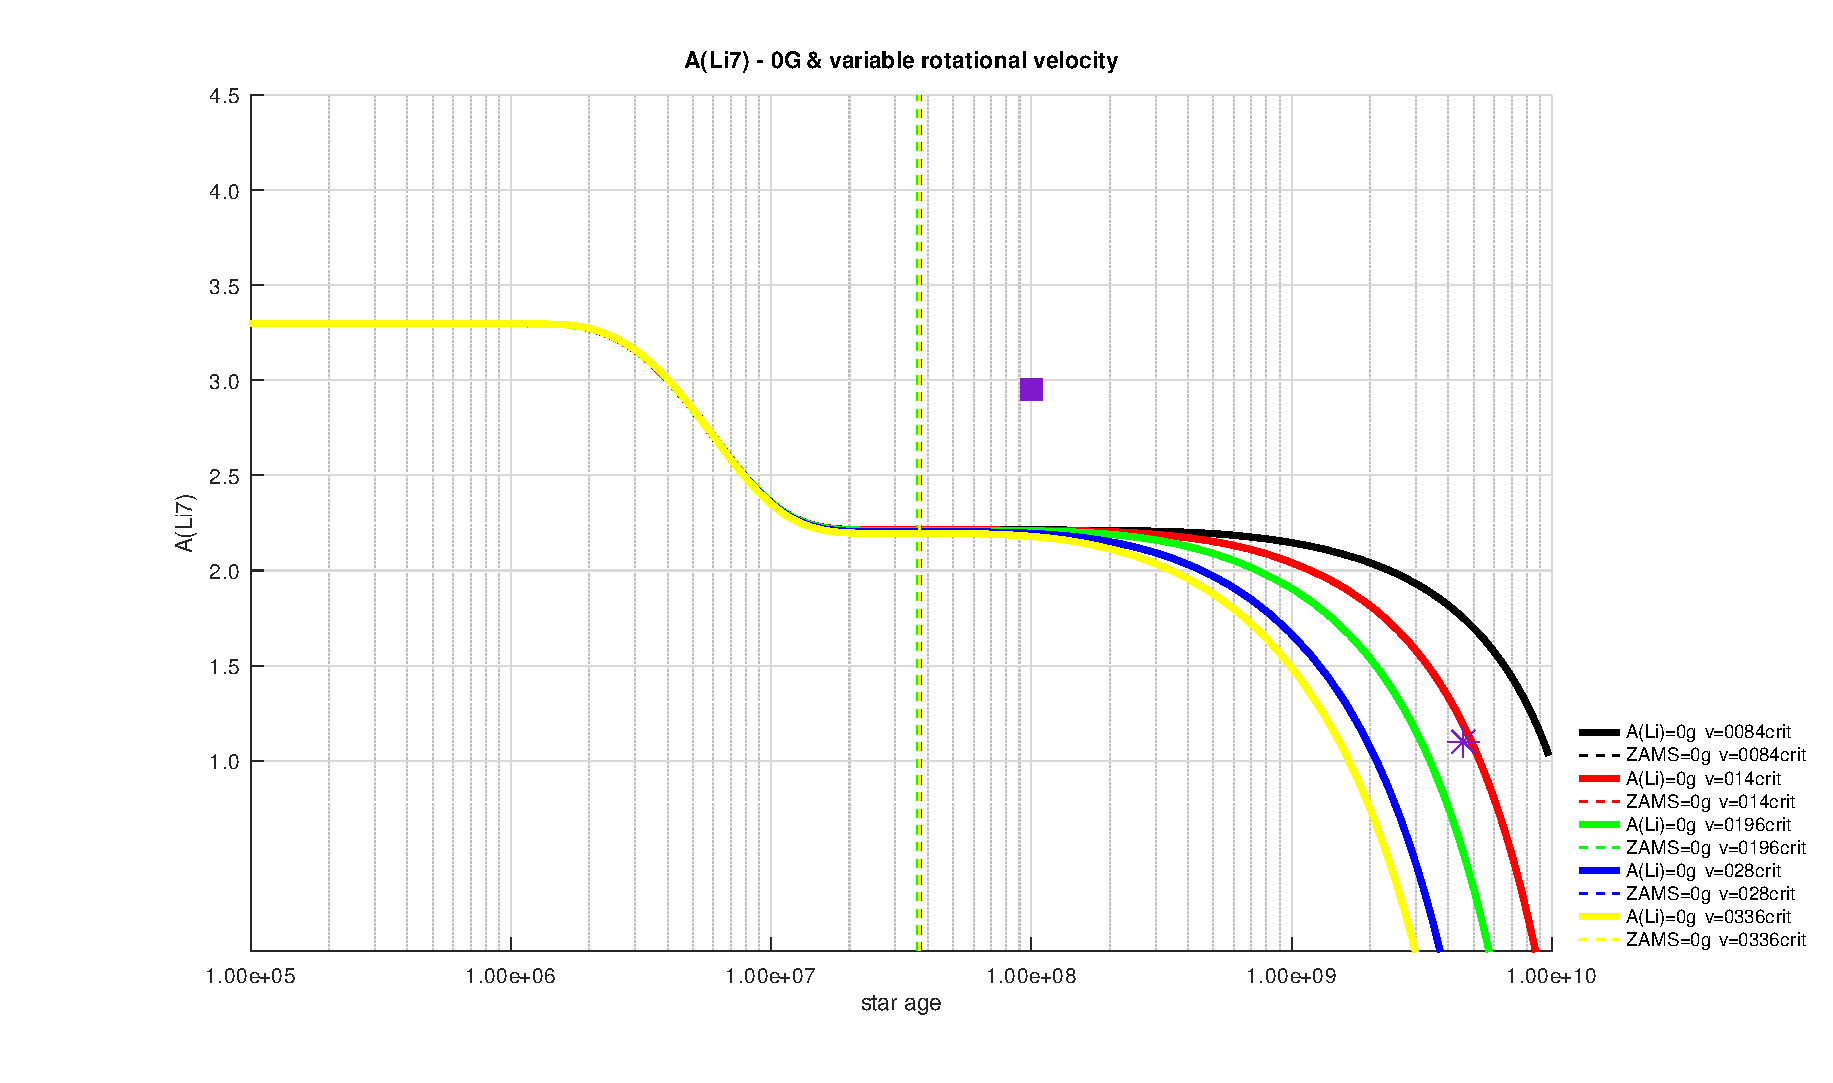
\includegraphics[trim = 40mm 15mm 20mm 15mm, clip, width=\columnwidth]{figures/li_var_vel_0_0g.eps}
    \caption{The evolution of surface \isotope[7]{Li} abundance relative to \isotope[1]{H}, as a function of time for several 1 $M_{\sun}$ models. The solid black line represents the reference model according to \citet{Choi2016}. The rest of lines are models which include PMS rotation with $\Omega / \Omega_{crit}$ between 0.0084 and 0.0336, respectively. The purple star and square are surface Li abundance for the present-day Sun \citep{Asplund2009} and the Pleiades cluster \citep{Sestito2005} respectively. The dashed lines make reference to the ZAMS.}
    \label{fig:li_var_vel_0g}
\end{figure}

Today, standard models are not able to replicate in a satisfactory way the observed values of Li abundance on star surfaces with the predictions that these models yield. This lack of agreement makes us think that certain physical mechanisms that influence the destruction of Li are either being modelled improperly or simply not being taken into account, e.g. the magnetic braking. Figure (\ref{fig:li_var_vel_0g}) shows the evolution of surface Li abundance relative to H as a function of time and for several $1M_{\odot}$ models which take into account the effects of rotation and AML caused by stellar winds but not MB. The purple star and square are surface Li abundances for the present-day Sun \citep{Asplund2009} and Pleiades \citep{Sestito2005}.\par

The figure (\ref{fig:li_var_vel_0g}) clearly allows to appreciate how the Li abundance in the star surface decreases over time for all simulated models. The solid black line represents the reference model that adopts the solar-calibrated envelope overshooting parameters as documented in \citet{Choi2016}. In general, all models burn too much Li before the ZAMS \footnote{Defined as the temporal simulation instant closest to the timestep in which both the central H mass fraction has been reduced by 0.0015 from its initial value and the model first $L_H/L_{phot} \geq 0.99$, where $L_{H}$ is luminosity produced by the H burning power at the star core and $L_{phot}$ represents the star luminosity in the photosphere.} and therefore do not match with the Pleiades surface Li abundance. Later, the reference model does not deplete Li efficiently on the MS and fail (again) to match the current solar surface Li abundance. On the other hand, the other models which include rotation during the PMS with values of $\Omega / \Omega_{crit}$ between 0.0084 and 0.0336 are able to burn Li in a more realistic way although only one of them (green line) is close to match the present-day Li abundance of the Sun but it rotational velocity is much higher (see figure (\ref{fig:rot_vel_0g})) than the $2\,kms^{-1}$ of the Sun \citep{Gill2012}. \par

For much of the PMS the star rotates as a solid body (see figure (\ref{fig:rot_vel_0g})) and this is because the star has a completely convective interior. It is not until the end of Hayashi track that the star begins to develop a radiative core due to the increase in temperature that occurs inside the star during the contraction process. It is in this stage of evolution of the star when a difference in angular velocity appears between the upper and lower limits of the radiative and convective zones respectively. The degree of differential rotation is directly influenced by the initial $\Omega$. As the models are initialized with a higher angular velocity, the difference in velocity between the BCZ and the star surface is accentuated in a directly proportional mode; the higher the initial velocity, the bigger the velocity gradient between the bottom and top limits of the CZ. As a consequence, the turbulence strength located at the BCZ increases so that Li can reach regions with temperatures about $T_{Li}$ where it is finally burned and destroyed (see figure (\ref{fig:li_var_vel_0g})). 

We would also like to point out that there are other investigations in which the conclusions obtained seem to point to a tendency diametrically opposed to the one exposed here, that is to say, the faster the rotation speed, the greater the abundance of Li on the surface of the star. An example of this is \citet{Bouvier2018} work in which the authors analyse the possible connection between the Li and the periods of rotation of FGK type stars present in the Pleiades cluster. Particularly interesting is the relationship found of a greater abundance of Li in the faster stars and a smaller one in the slower ones. A possible hypothesis proposed to explain these observations would suggest that the effects of rotation in those stars that rotate faster makes the overshooting effect less efficient and therefore less material of the convective envelope reaches the radiative core where there is enough temperature to destroy the Li \citep{Baraffe2017}. Another possibility exposes that stars with slow rotation develop a higher level of differential rotation, so that a higher Li destruction is expected \citep{Bouvier2008}. Also remarkable from the results offered by the numerical simulations is the fact that there are barely any differences between the different models in terms of the abundance of Li for much of the PMS. It is not until about $10^7$ years that the differences begin to be most noticeable (see figure (\ref{fig:li_var_vel_0g_z1})).\par

\begin{figure}
	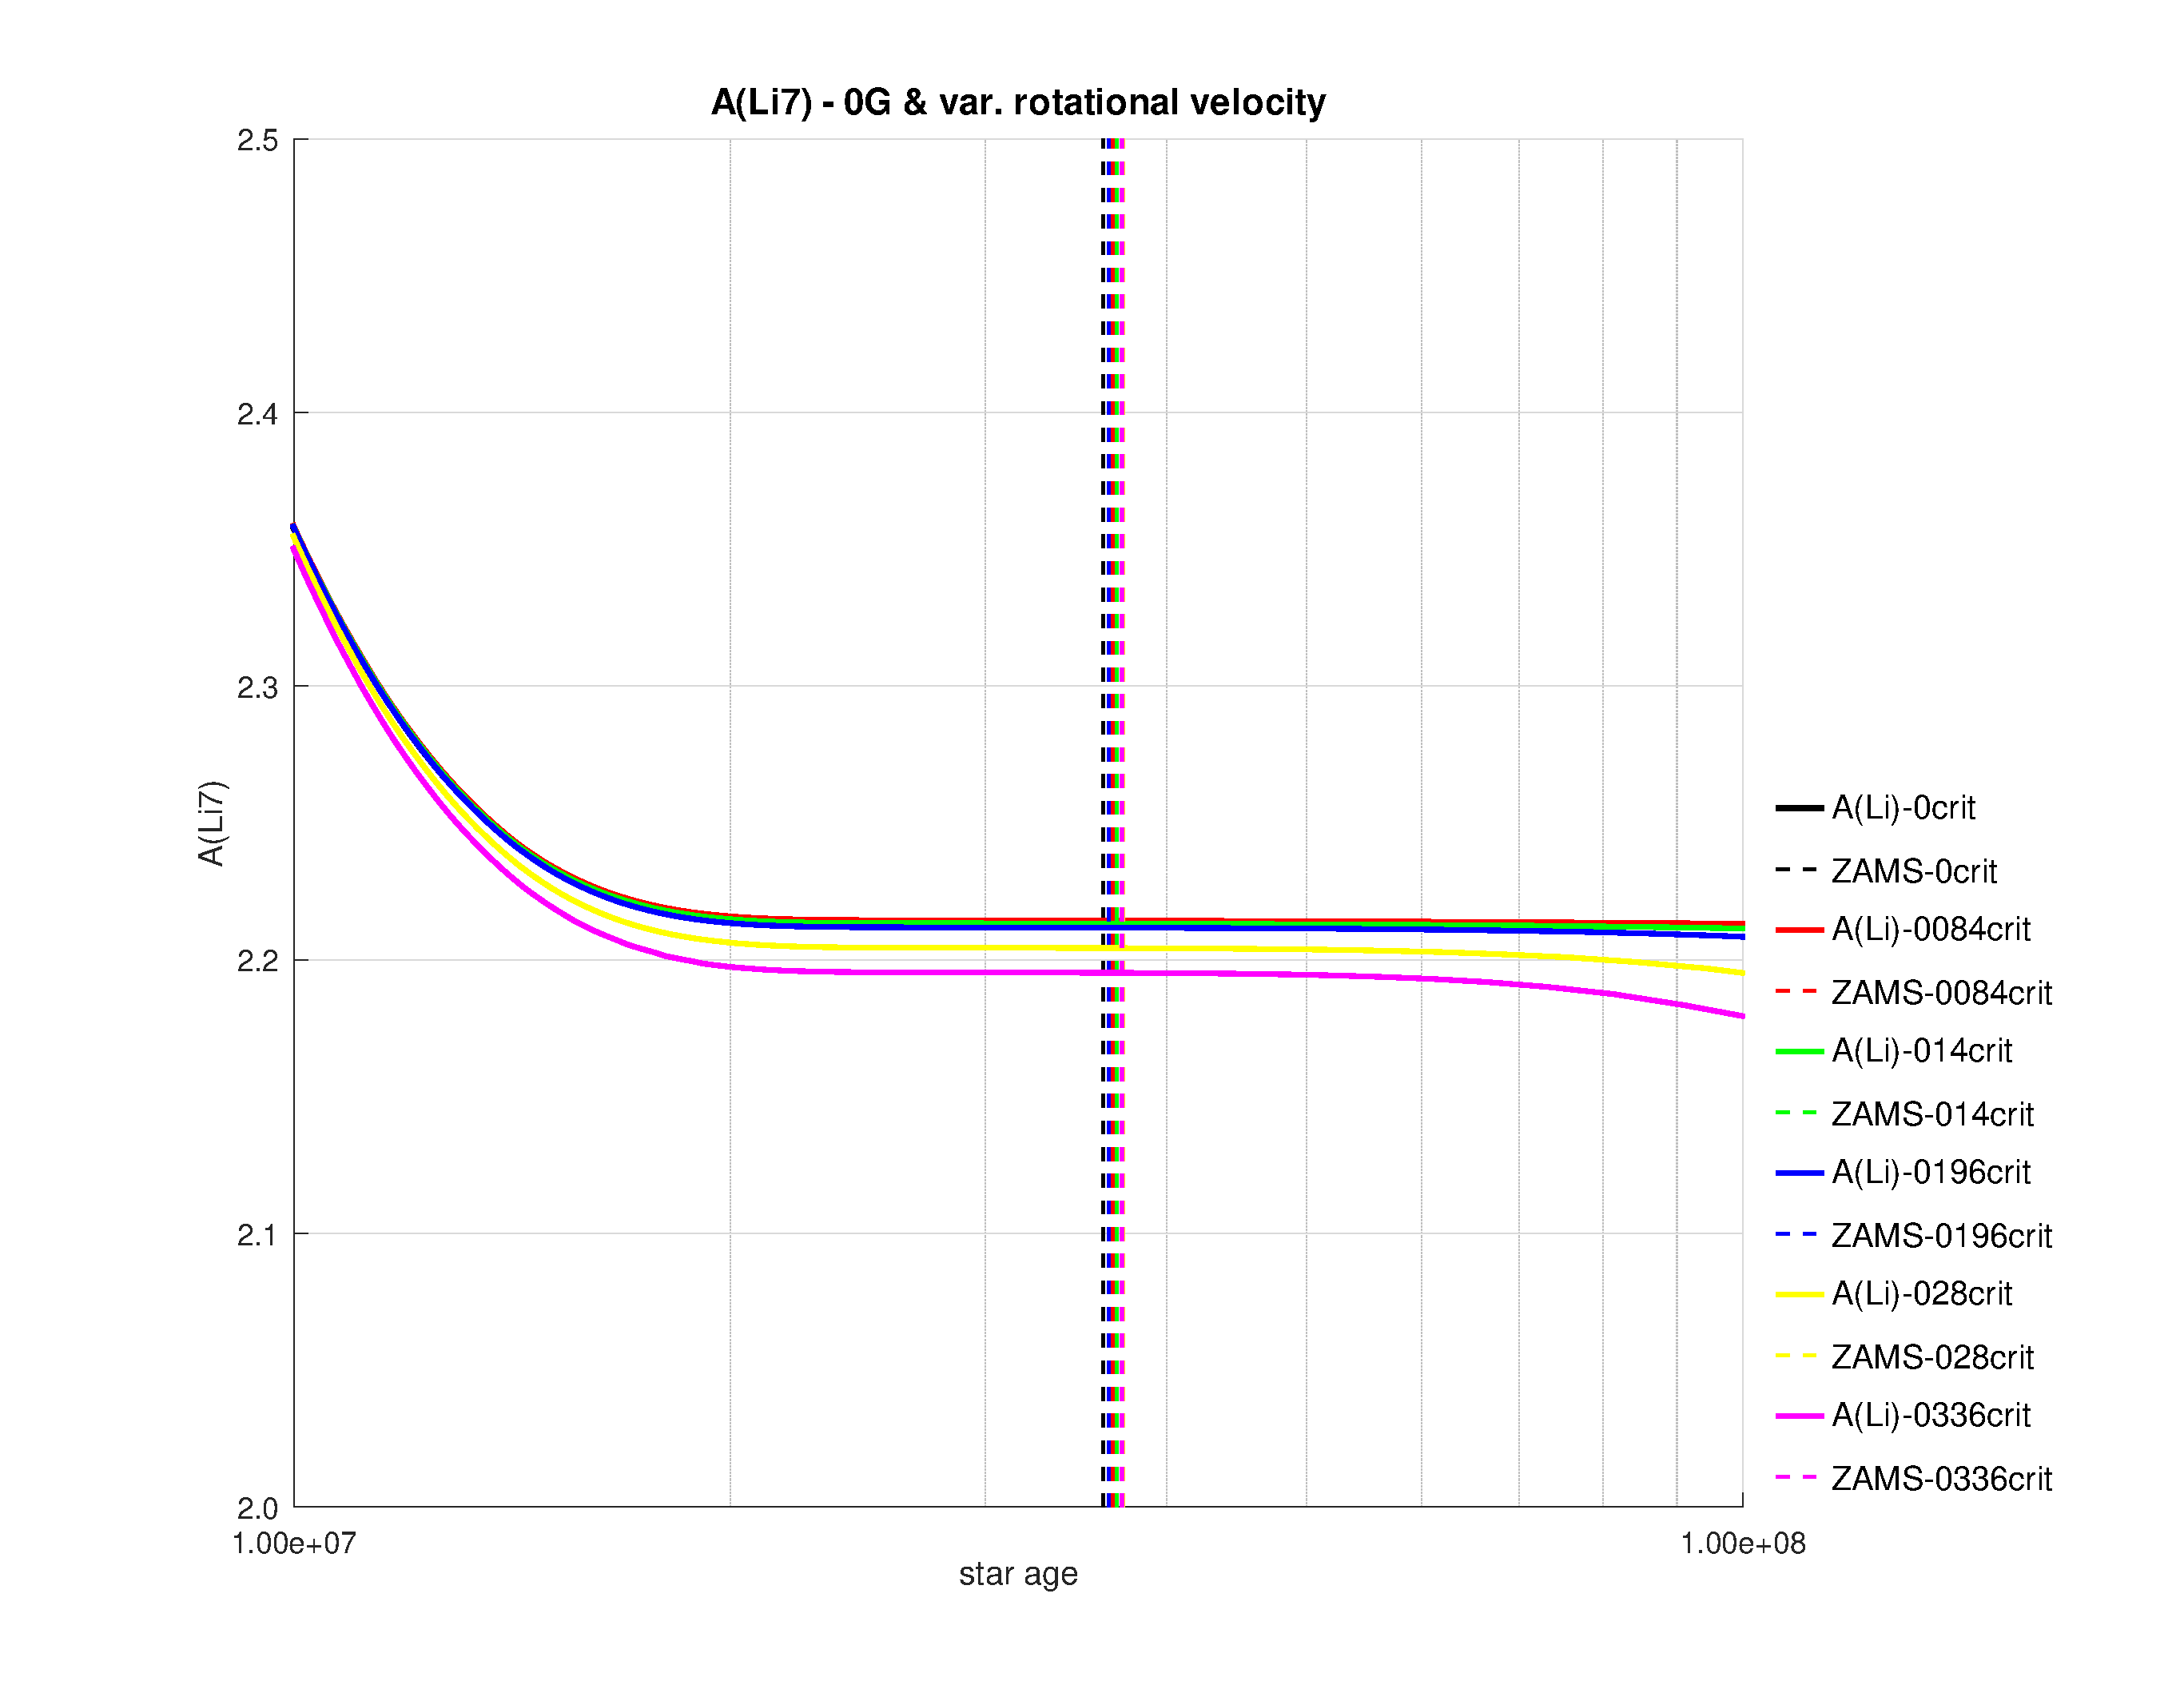
\includegraphics[trim = 40mm 15mm 20mm 15mm, clip,width=\columnwidth]{figures/li_var_vel_0_0g_z1.eps}
    \caption {Similar to figure (\ref{fig:li_var_vel_0g}) but zooming in on the ZAMS. The models with a higher initial rotational velocity reach already the ZAMS with a lower amount of Li measure on the star surface.}
    \label{fig:li_var_vel_0g_z1}
\end{figure}

\begin{figure}
	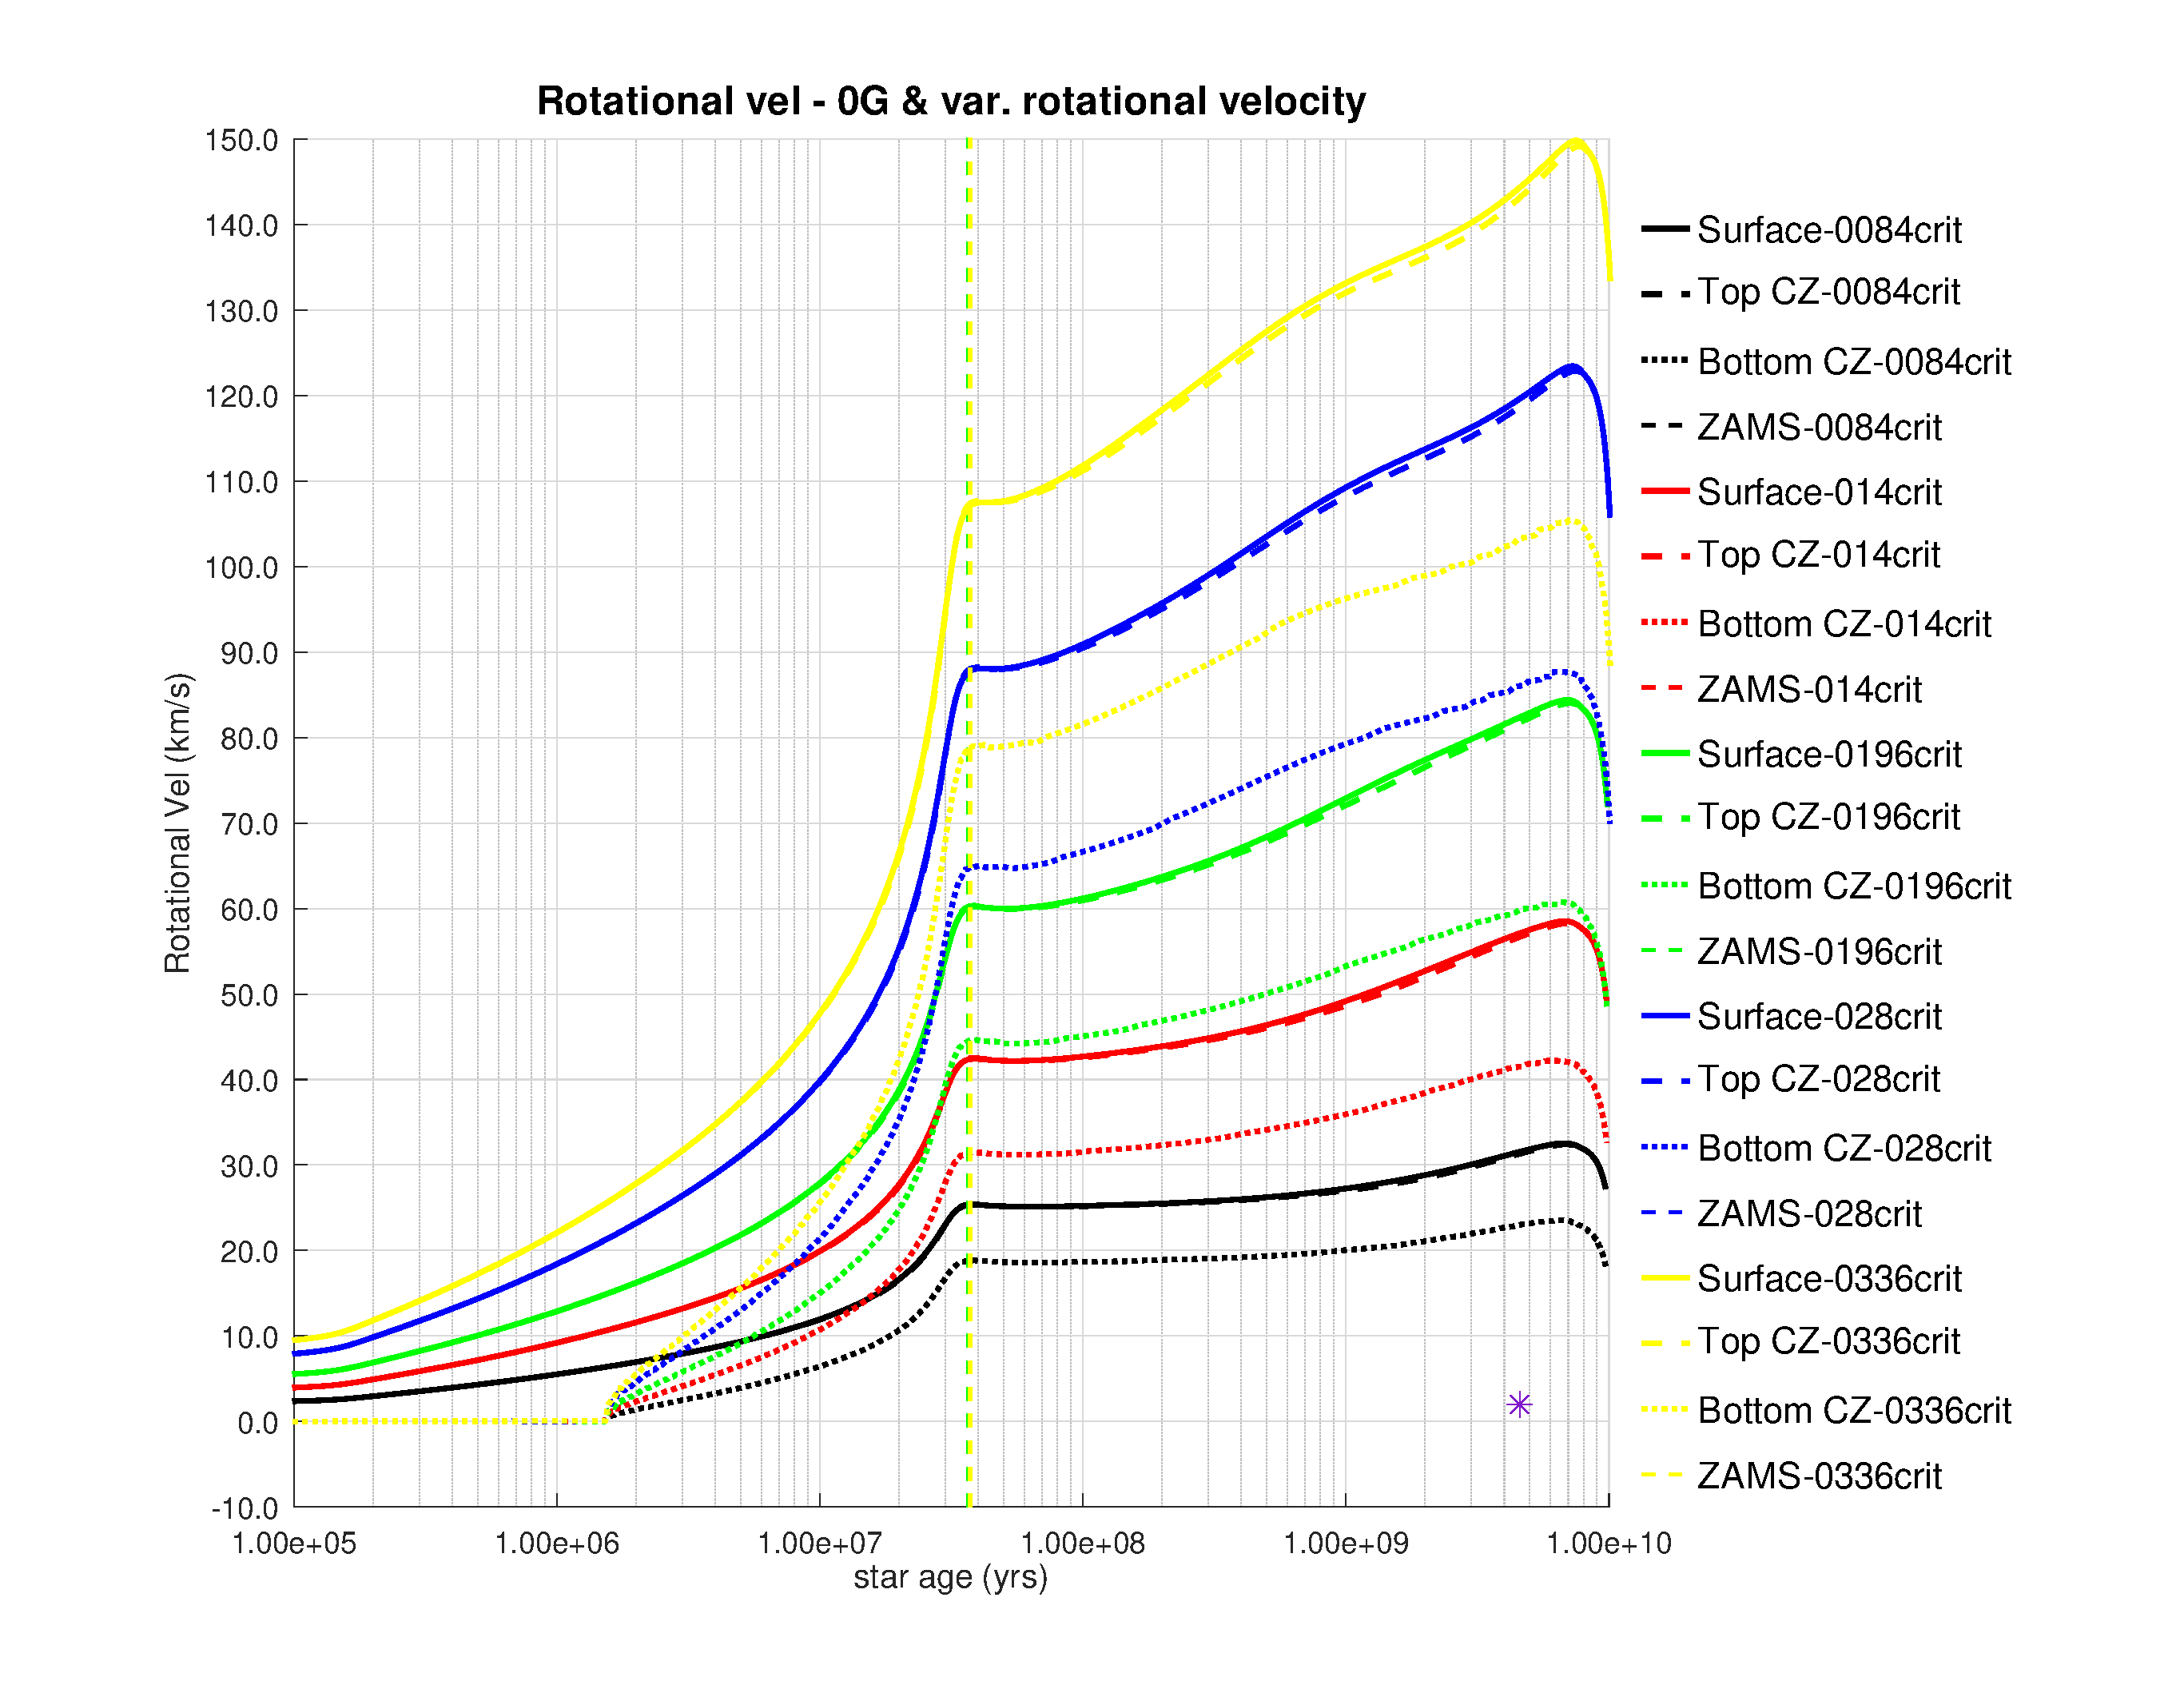
\includegraphics[trim = 40mm 15mm 20mm 15mm, clip,width=\columnwidth]{figures/rot_vel_var_vel_0_0g.eps}
    \caption{The evolution of angular velocity at surface (solid line) and the top (dashed line) and bottom (dotted line) limits of the uppermost convective zone, as a function of time for several 1 $M_{\sun}$ models. The models includes PMS rotation with $\Omega / \Omega_{crit}$ values between 0.0084 and 0.0336. The purple star is the surface angular velocity for the present-day Sun \citep{Gill2012}. The dashed vertical lines make reference to the ZAMS.}
    \label{fig:rot_vel_0g}
\end{figure}

Another well known structural effect of rotation is the decrease of the effective temperature ($T_{eff}$) and to a less extent of stellar luminosity ($L$). Both effects can be observed graphically in the HR diagram of figure (\ref{fig:hr_var_vel_0g}) which shows a zoomed-in view of evolution tracks from the ZAMS till the TAMS. If we compare the non-rotating model (black solid line on the left side) with the rotating ones we can recognize that at the end of the PMS, the latter reach before the ZAMS and exhibit a lower $T_{eff}$ than the former. These results are in line with those of previous studies (see e.g. \citet{Eggenberger2012}, \citet{Piau2001}, \citet{Pinsonneault1989}).\par


\begin{figure}
	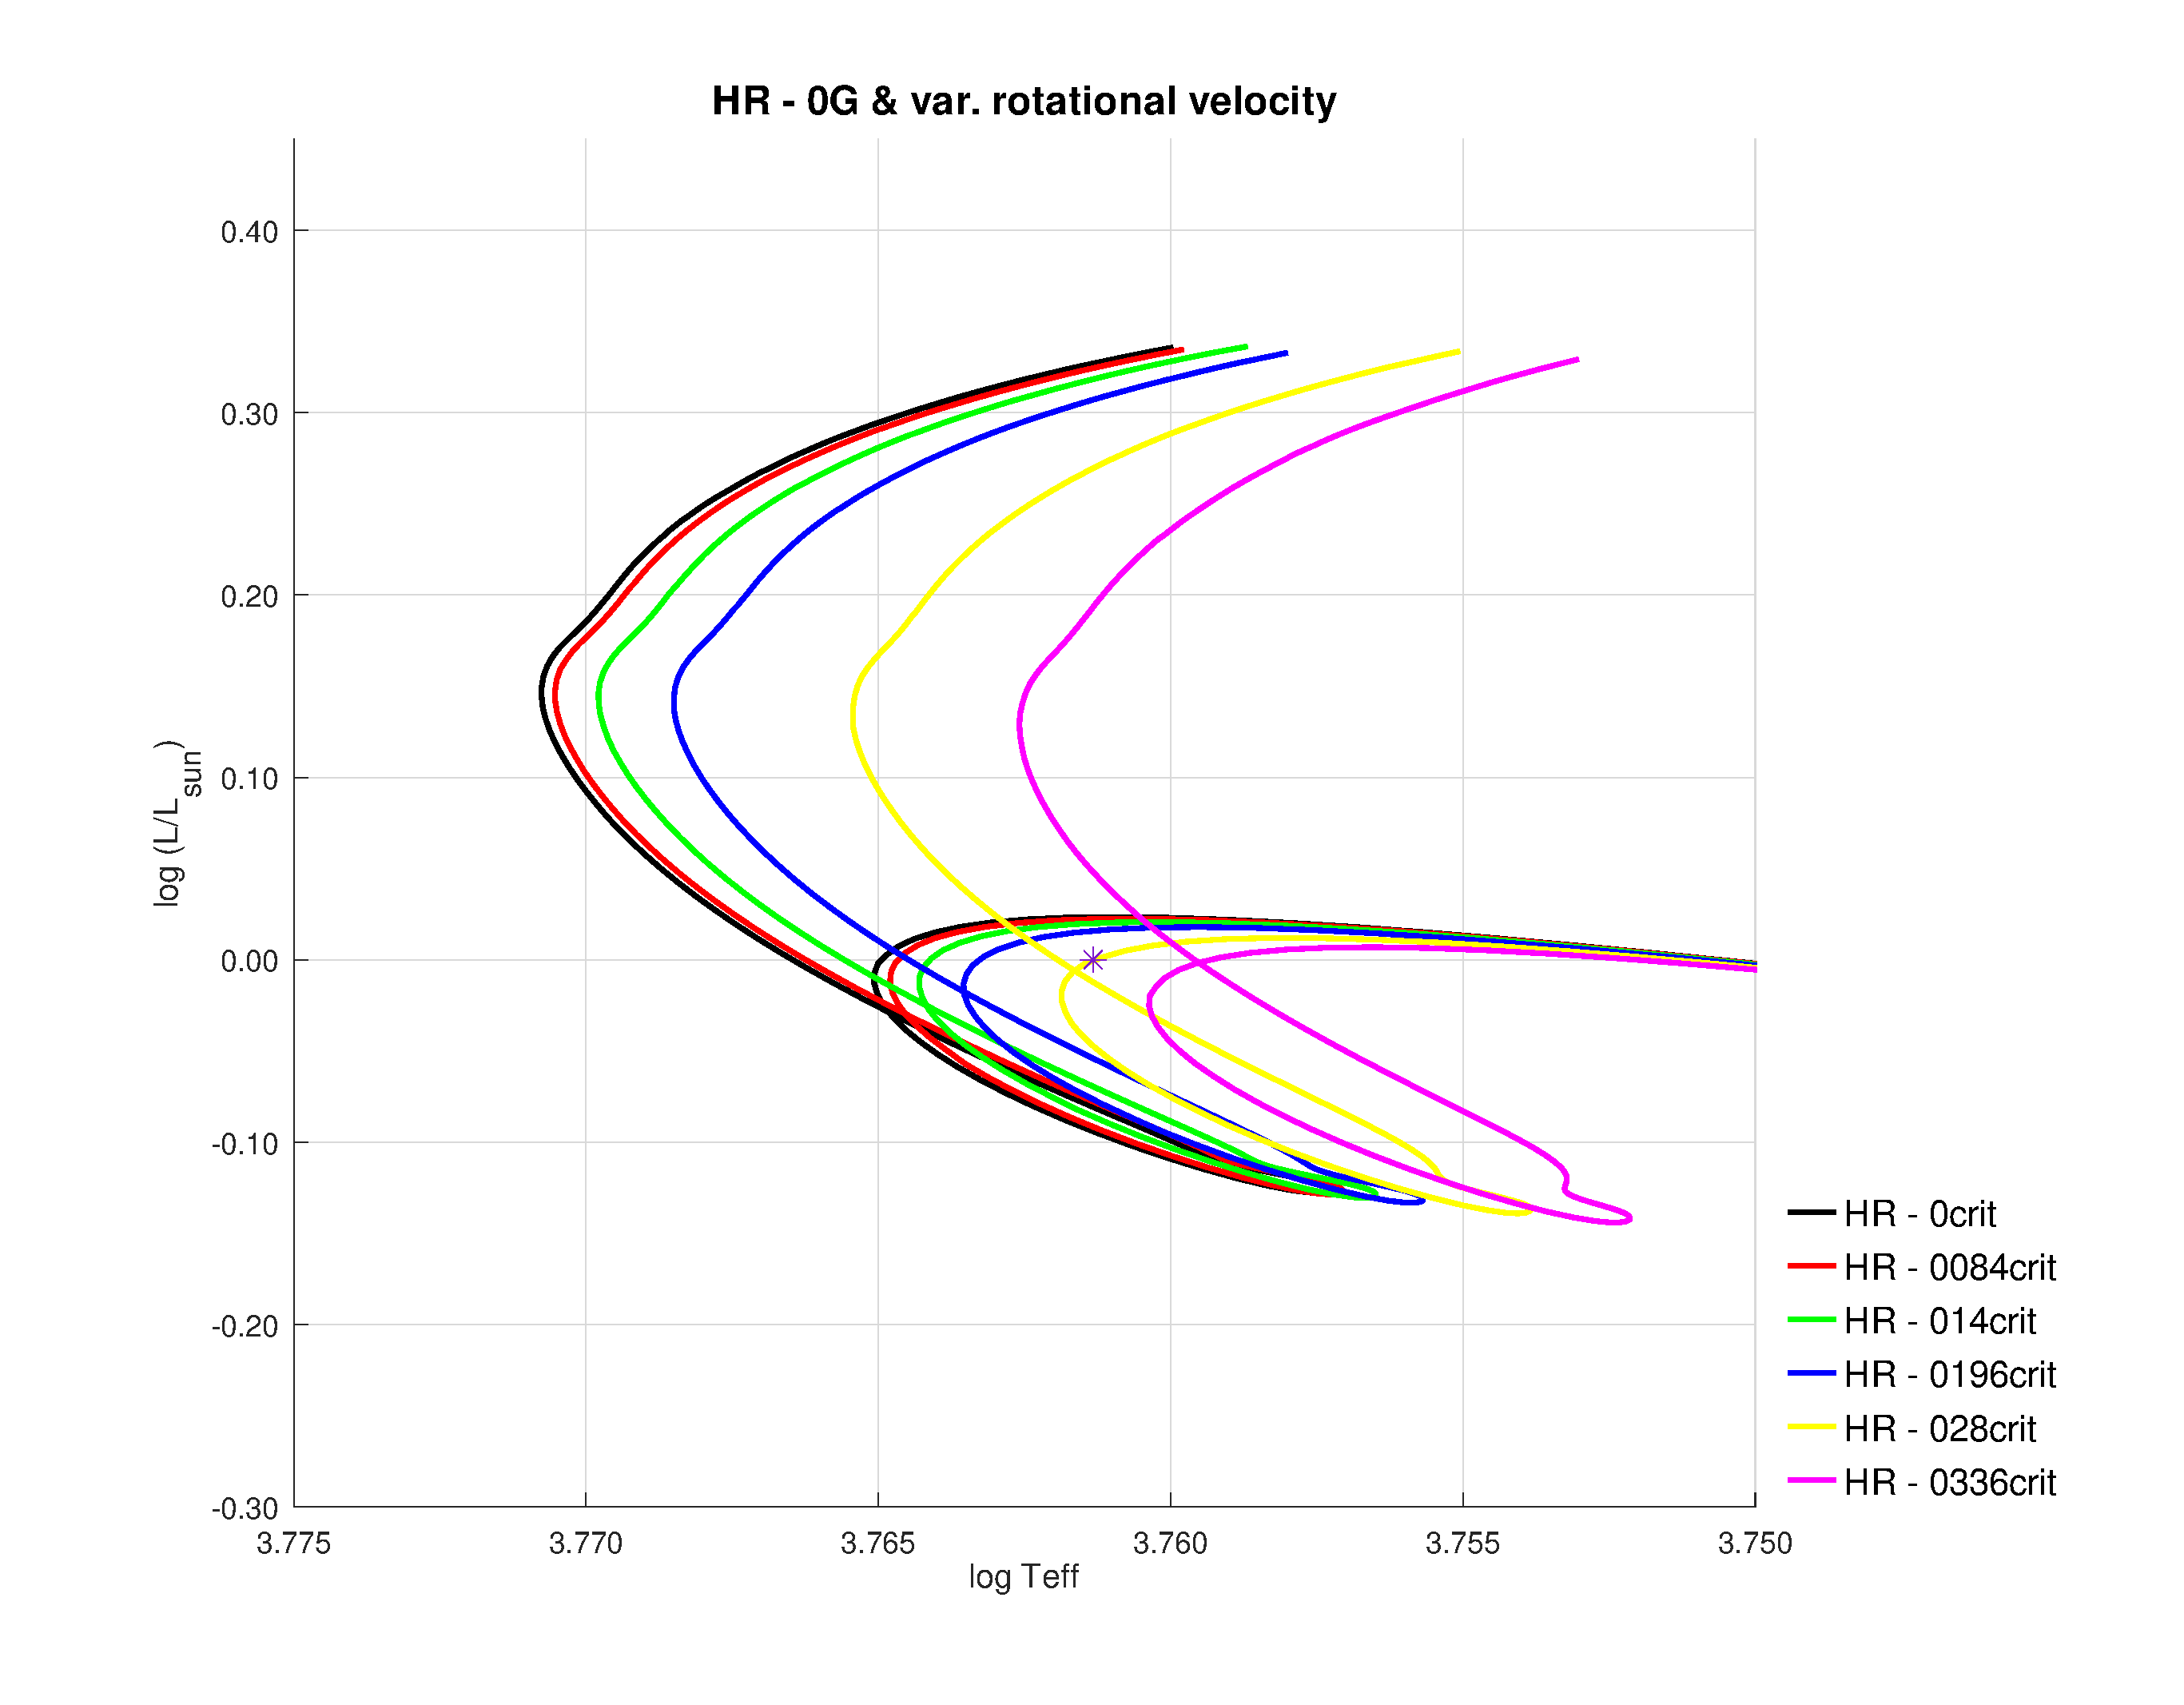
\includegraphics[trim = 30mm 15mm 20mm 15mm, clip,width=\columnwidth]{figures/hr_var_vel_0_0g_z1.eps}
    \caption{An example solar 1$M_{\sun}$ grid of stellar evolutionary track from PMS till TAMS covering a wide range of angular velocities. The rotation is activated in the models in the PMS and those models reach before the ZAMS and at a lower $T_{eff}$ than the non-rotating one (solid black line). The luminosity is expressed in terms of $L_{\sun}$}.
    \label{fig:hr_var_vel_0g}
\end{figure}

\subsection{Magnetic braking, Li abundance and effective temperature}
In the rest of this document we are going to focus, unless otherwise indicated, on models that include rotation from the PMS since they are the ones that can offer a greater approximation to the observations. In turn, these models will serve as a basis for others in which our magnetic braking routine is used by simulating magnetic fields of different intensity, varying from 3.5G to 5.5G in 0.5G increments.\par

If we concentrate our attention on figure (\ref{fig:li_var_vel_4_0g}) and compare it with figure (\ref{fig:li_var_vel_0g}) we will see how the profiles of Li abundance are altered during PMS and MS. In the first phase we can describe the effect as modest, somewhat expected and in line with the fact that the AML caused by MB (see equation (\ref{eq:j_dot})) depends directly on the loss of mass. If we take into account that for solar-type stars the models predict a modest total loss of mass, that value is even much lower during PMS. On the contrary, during the MS it is observed that the AML is much more significant, causing the star to rotate more slowly and as a result a smaller amount of Li to be destroyed.\par

\begin{figure}
	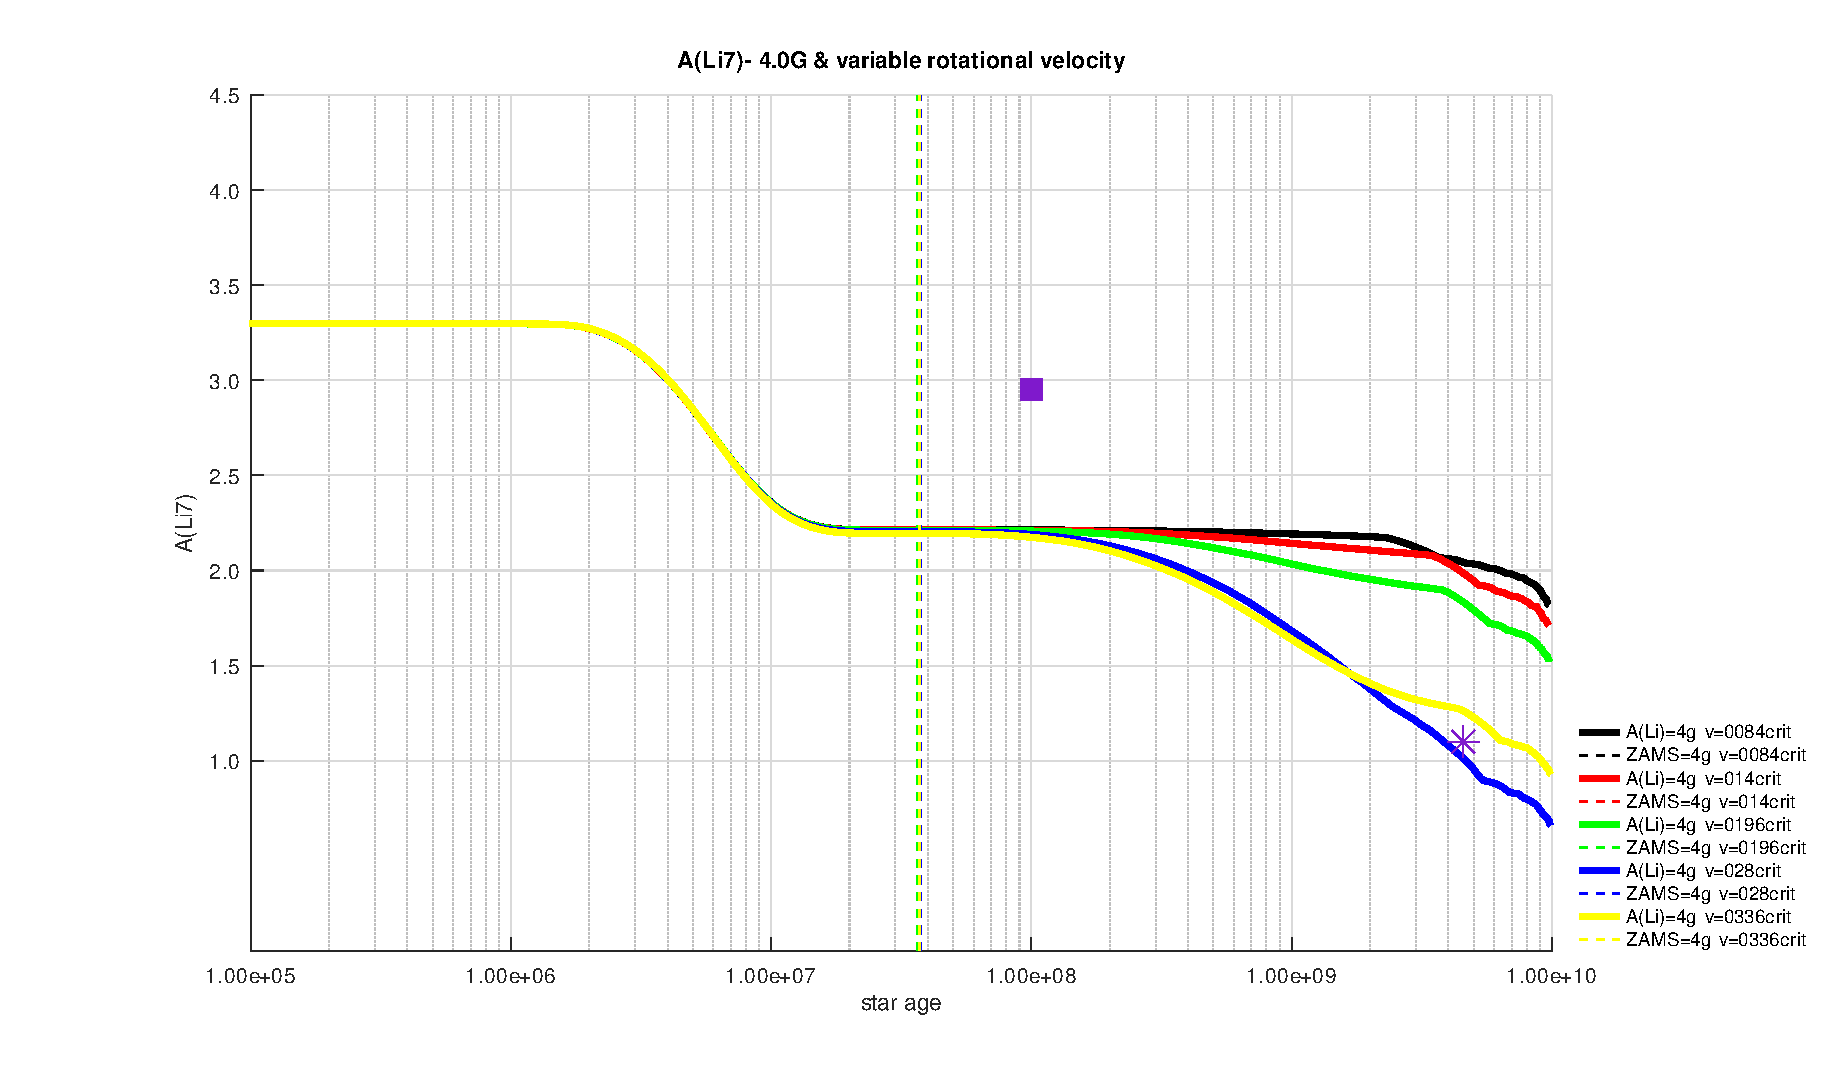
\includegraphics[trim = 40mm 15mm 20mm 15mm, clip,width=\columnwidth]{figures/li_var_vel_4_0g.eps}
    \caption{The evolution of surface \isotope[7]{Li} abundance relative to \isotope[1]{H}, as a function of time for several 1 $M_{\sun}$ models. The models include a magnetic field with an intensity of 4G and PMS rotation with $\Omega / \Omega_{crit}$ between 0.0084 and 0.0336, respectively. The purple star and square are surface Li abundance for the present-day Sun \citep{Asplund2009} and the Pleiades cluster \citep{Sestito2005} respectively. The dashed lines make reference to the ZAMS.}
    \label{fig:li_var_vel_4_0g}
\end{figure}

The effect of the MB routine can be seen even more clearly in figures (\ref{fig:rot_vel_4g}) \& (\ref{fig:grid_rot_vel}). Here we represent the rotation profiles on the surface of the stars for different rotating models. Similarly to the evolution profiles of the Li on the surface commented in the previous paragraph, the effect of the routine is much more accentuated once the ZAMS is reached. If we compare the evolution of the curves presented here with those of figure (\ref{fig:rot_vel_0g}) we see how the star, instead of continuing to increase its $\Omega$, begins to slow down after having reached its maximum in the passage through the ZAMS. These results are also consistent with those obtained by \citet{Eggenberger2010} as far as the effect of the magnetic field, in particular its influence on the loss of angular momentum, has on the rotational velocity of the star. In our models we have also chosen to include the rotation effects offered by MESA but not those of Tayler-Spruit dynamo on the diffusion of elements. In a similar way we also observe that the models with lower angular rotation generally end up exhibiting higher values in the abundance of Li on the surface (see figures (\ref{fig:li_var_vel_4_0g}), (\ref{fig:grid_li_var_vel}) \& (\ref{fig:grid_li_var_g})). In none of those cases we do obtain values of Li on the surface higher than those shown by the model without rotation.\par

We also find interesting to highlight the behaviour of $\Omega$ profiles when approaching TAMS. It can be recognized in figure (\ref{fig:rot_vel_4g}) and in more detail in (\ref{fig:rot_vel_4g_z1}), that its evolution suffers from a series of ups and downs that do not appear previously. Everything seems to indicate that this behavior is due to a combined effect of the MB routine and the time-step resolution (probably to big) used by MESA during the last part of the simulation. We based this affirmation on the fact that this effect is not observed in the series of simulations in which the routine is not included (see figure (\ref{fig:rot_vel_0g})).\par

\begin{figure}
	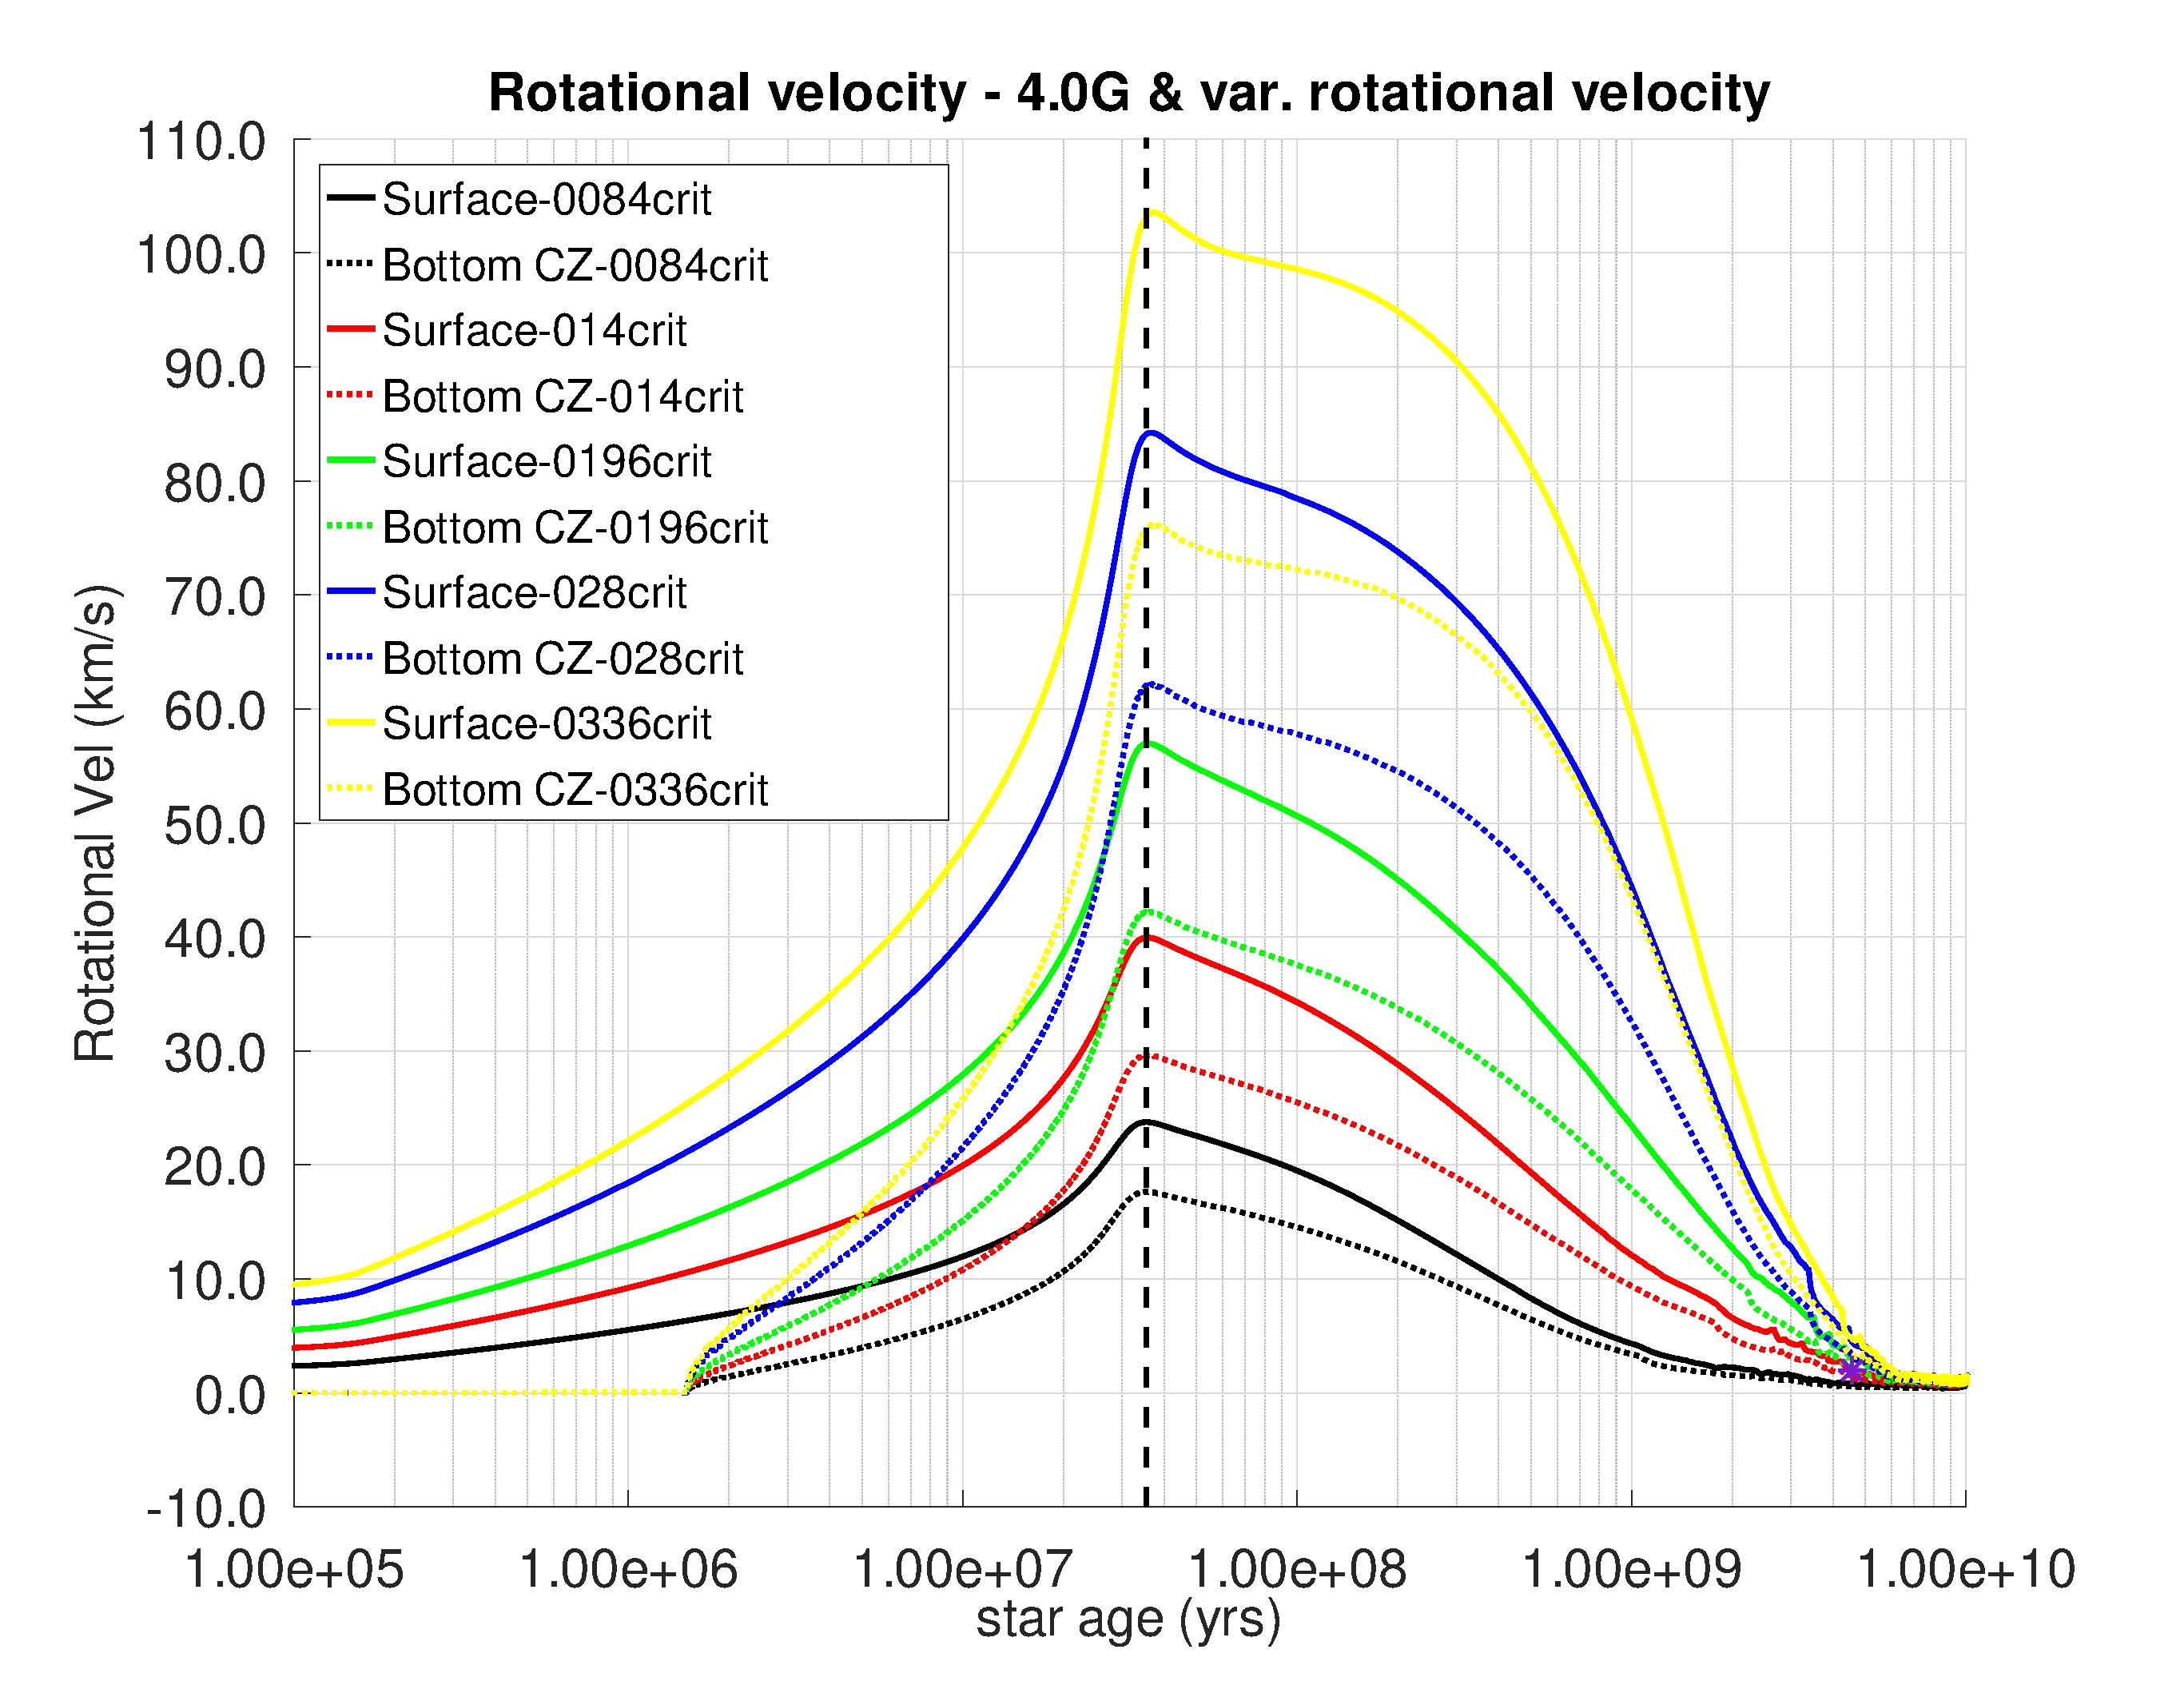
\includegraphics[trim = 30mm 15mm 20mm 15mm, clip,width=\columnwidth]{figures/rot_vel_var_vel_4_0g.eps}
    \caption{The evolution of surface rotational velocity, as a function of time for several 1 $M_{\sun}$ models. The models include a magnetic field with an intensity of 4G and PMS rotation with $\Omega / \Omega_{crit}$ between 0.0084 and 0.0336, respectively. Additionally it's simulated the magnetic braking effect of magnetic field with an intensity of 4G. The purple star is the surface angular velocity for the present-day Sun \citep{Gill2012}. The dashed lines make reference to the ZAMS.}
    \label{fig:rot_vel_4g}
\end{figure}

\begin{figure}
	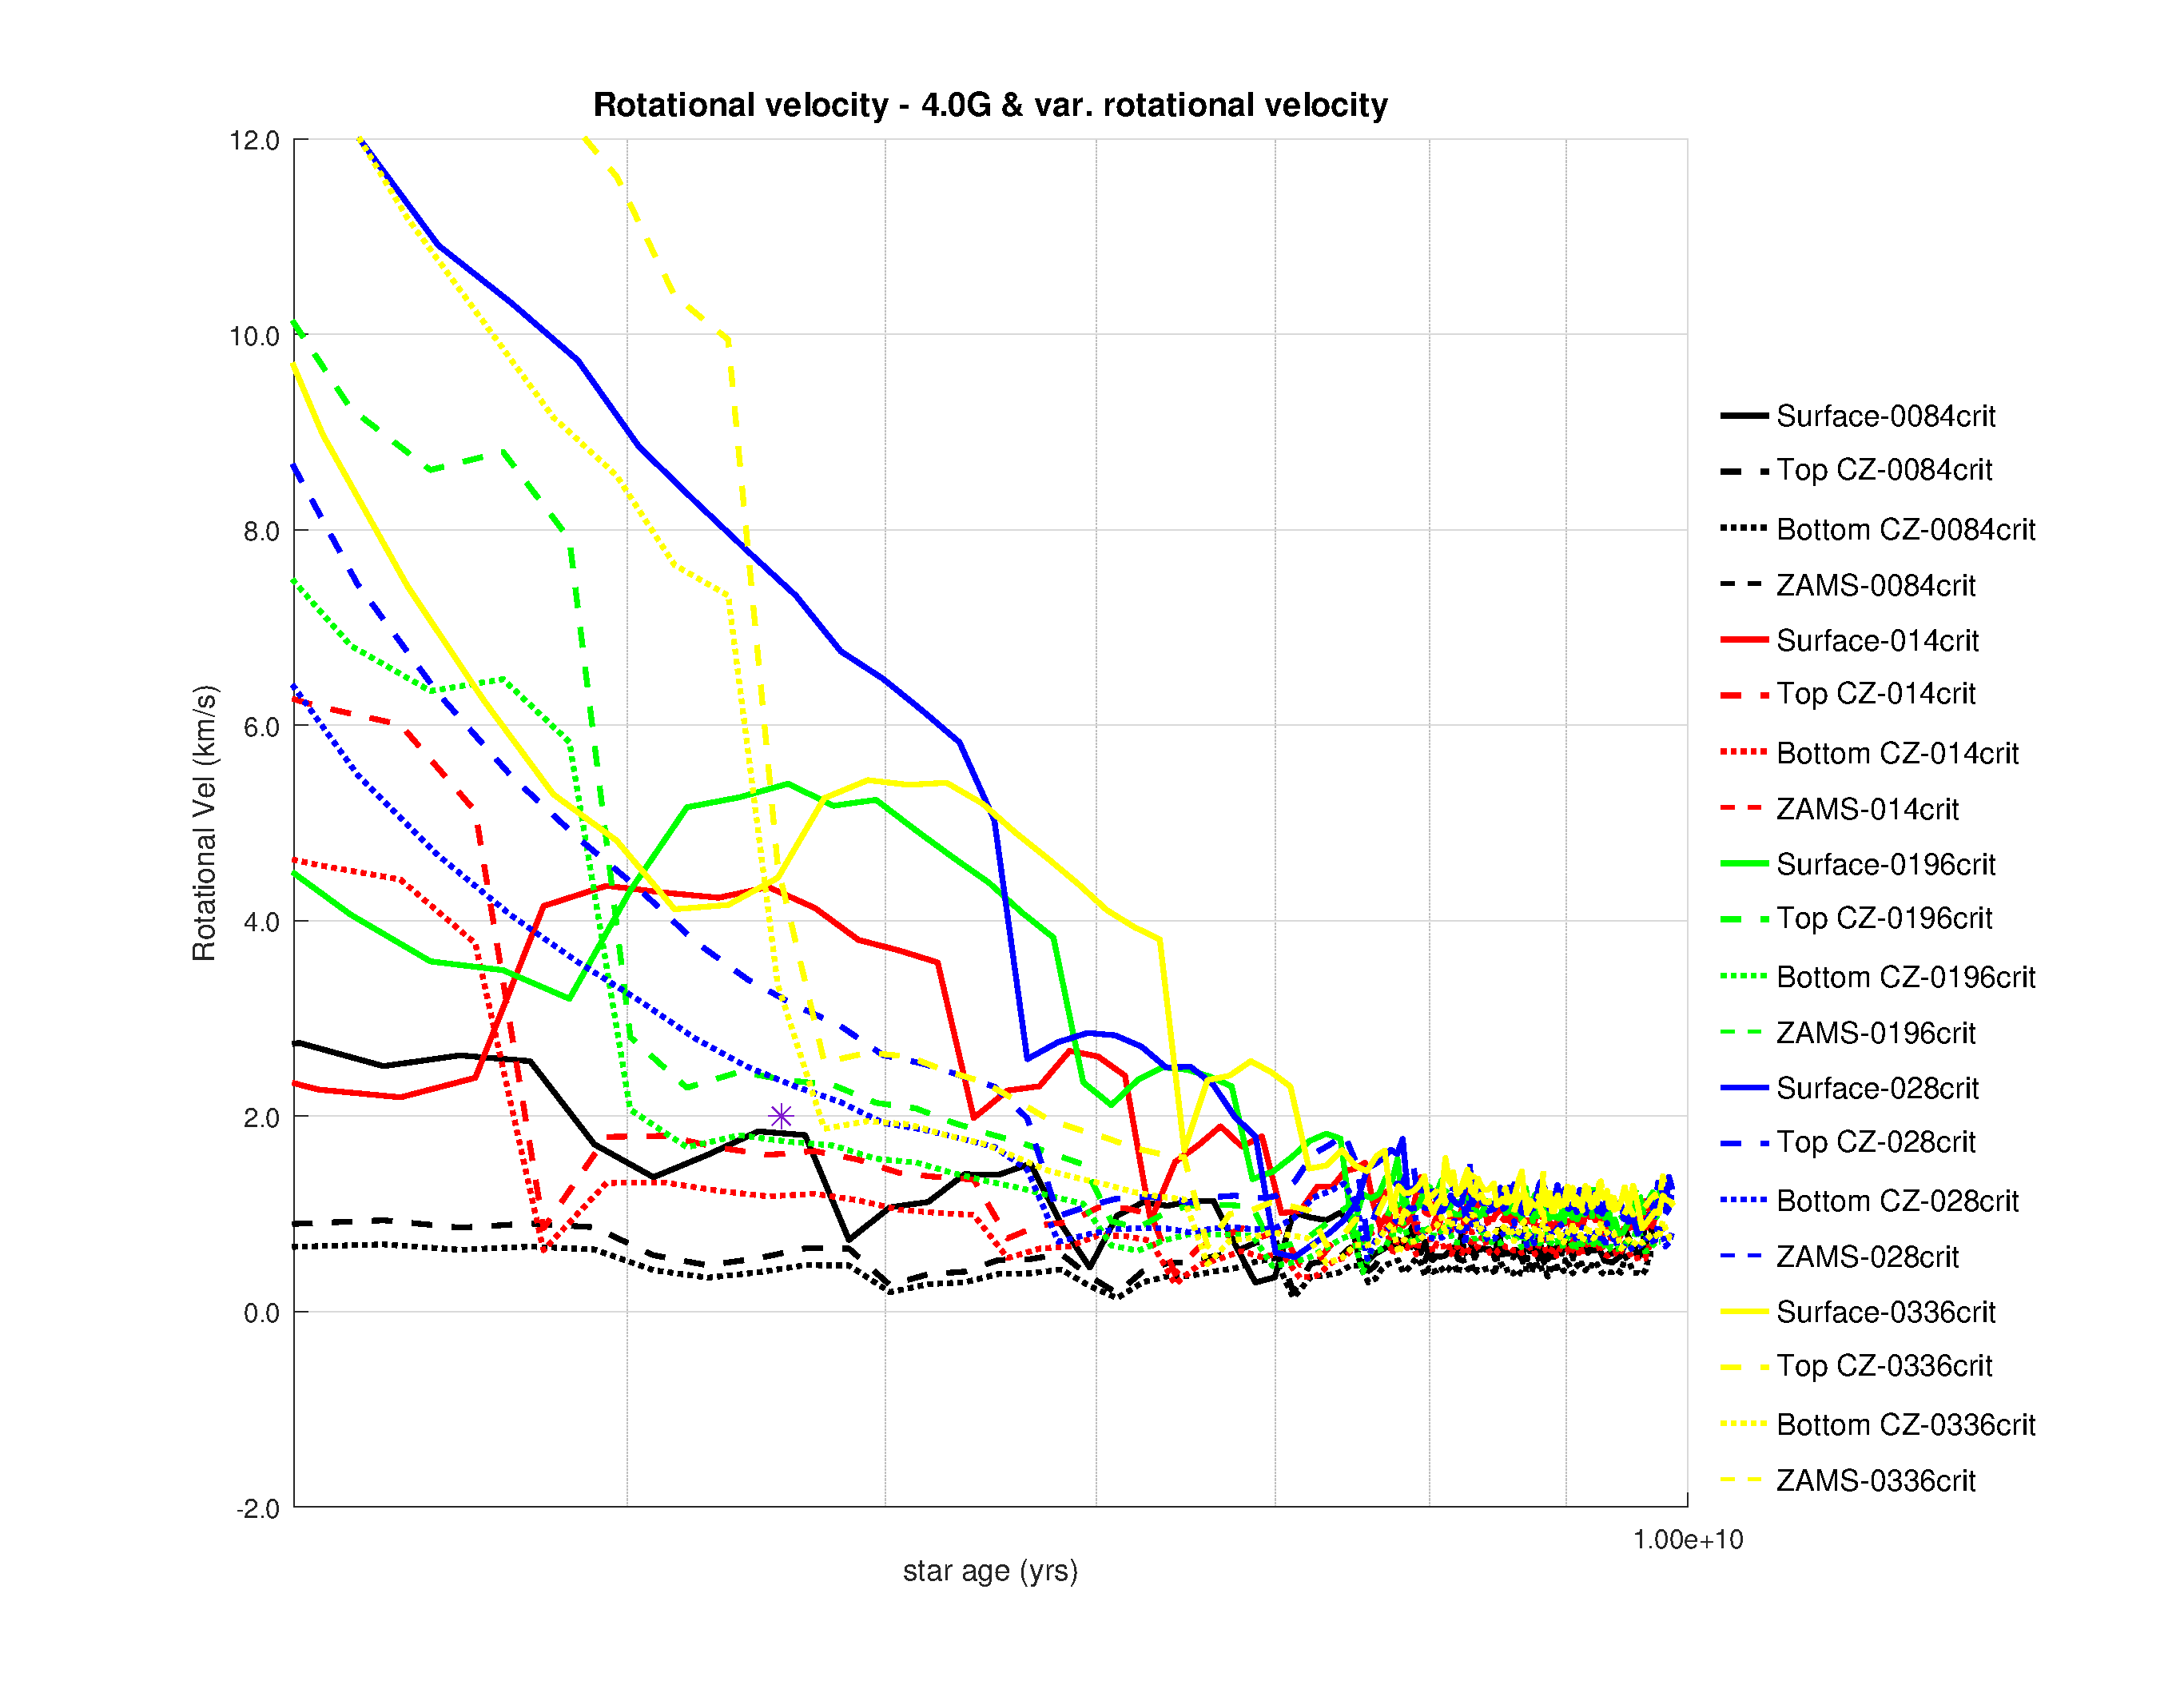
\includegraphics[trim = 30mm 15mm 20mm 15mm, clip,width=\columnwidth]{figures/rot_vel_var_vel_4_0g_z1.eps}
    \caption{Similar to figure (\ref{fig:rot_vel_4g}) but now showing in detail the surface rotational velocity as the star approaches TAMS.}
    \label{fig:rot_vel_4g_z1}
\end{figure}

It's also remarkable to observed, for some of the models depicted in figure (\ref{fig:rot_vel_4g}), the lower $\Omega$ at the star surface (solid line) in comparison with the upper limit of the convective layer (dashed line). This fact is most probably a consequence of the expansion of the superficial layers after the mass loss produced by stellar winds.\par

The MB also leaves its mark on the HR diagram by significantly affecting the $T_{eff}$ of the star. To visualize this effect we will take as reference figure (\ref{hr_vc_0336_var_g_z1}) in which all models were started with the same value $\Omega / \Omega_{crit}=0.0336$. In particular, let us pay attention to the evolutionary trace in which a magnetic field was not simulated (black solid line) and to the rest of the evolutionary traces in which it was. We have that the group of simulations with presence of a magnetic field produces hotter stars due to the MB influence. The lower speed with which the star rotates due to the MB effect causes the increase of the $T_{eff}$, being this difference of practically $95\,K$ between the simulated models with $0\,G$ and $5.5\,G$ respectively for $log(L/L_{\sun})=0$.

\begin{figure}
	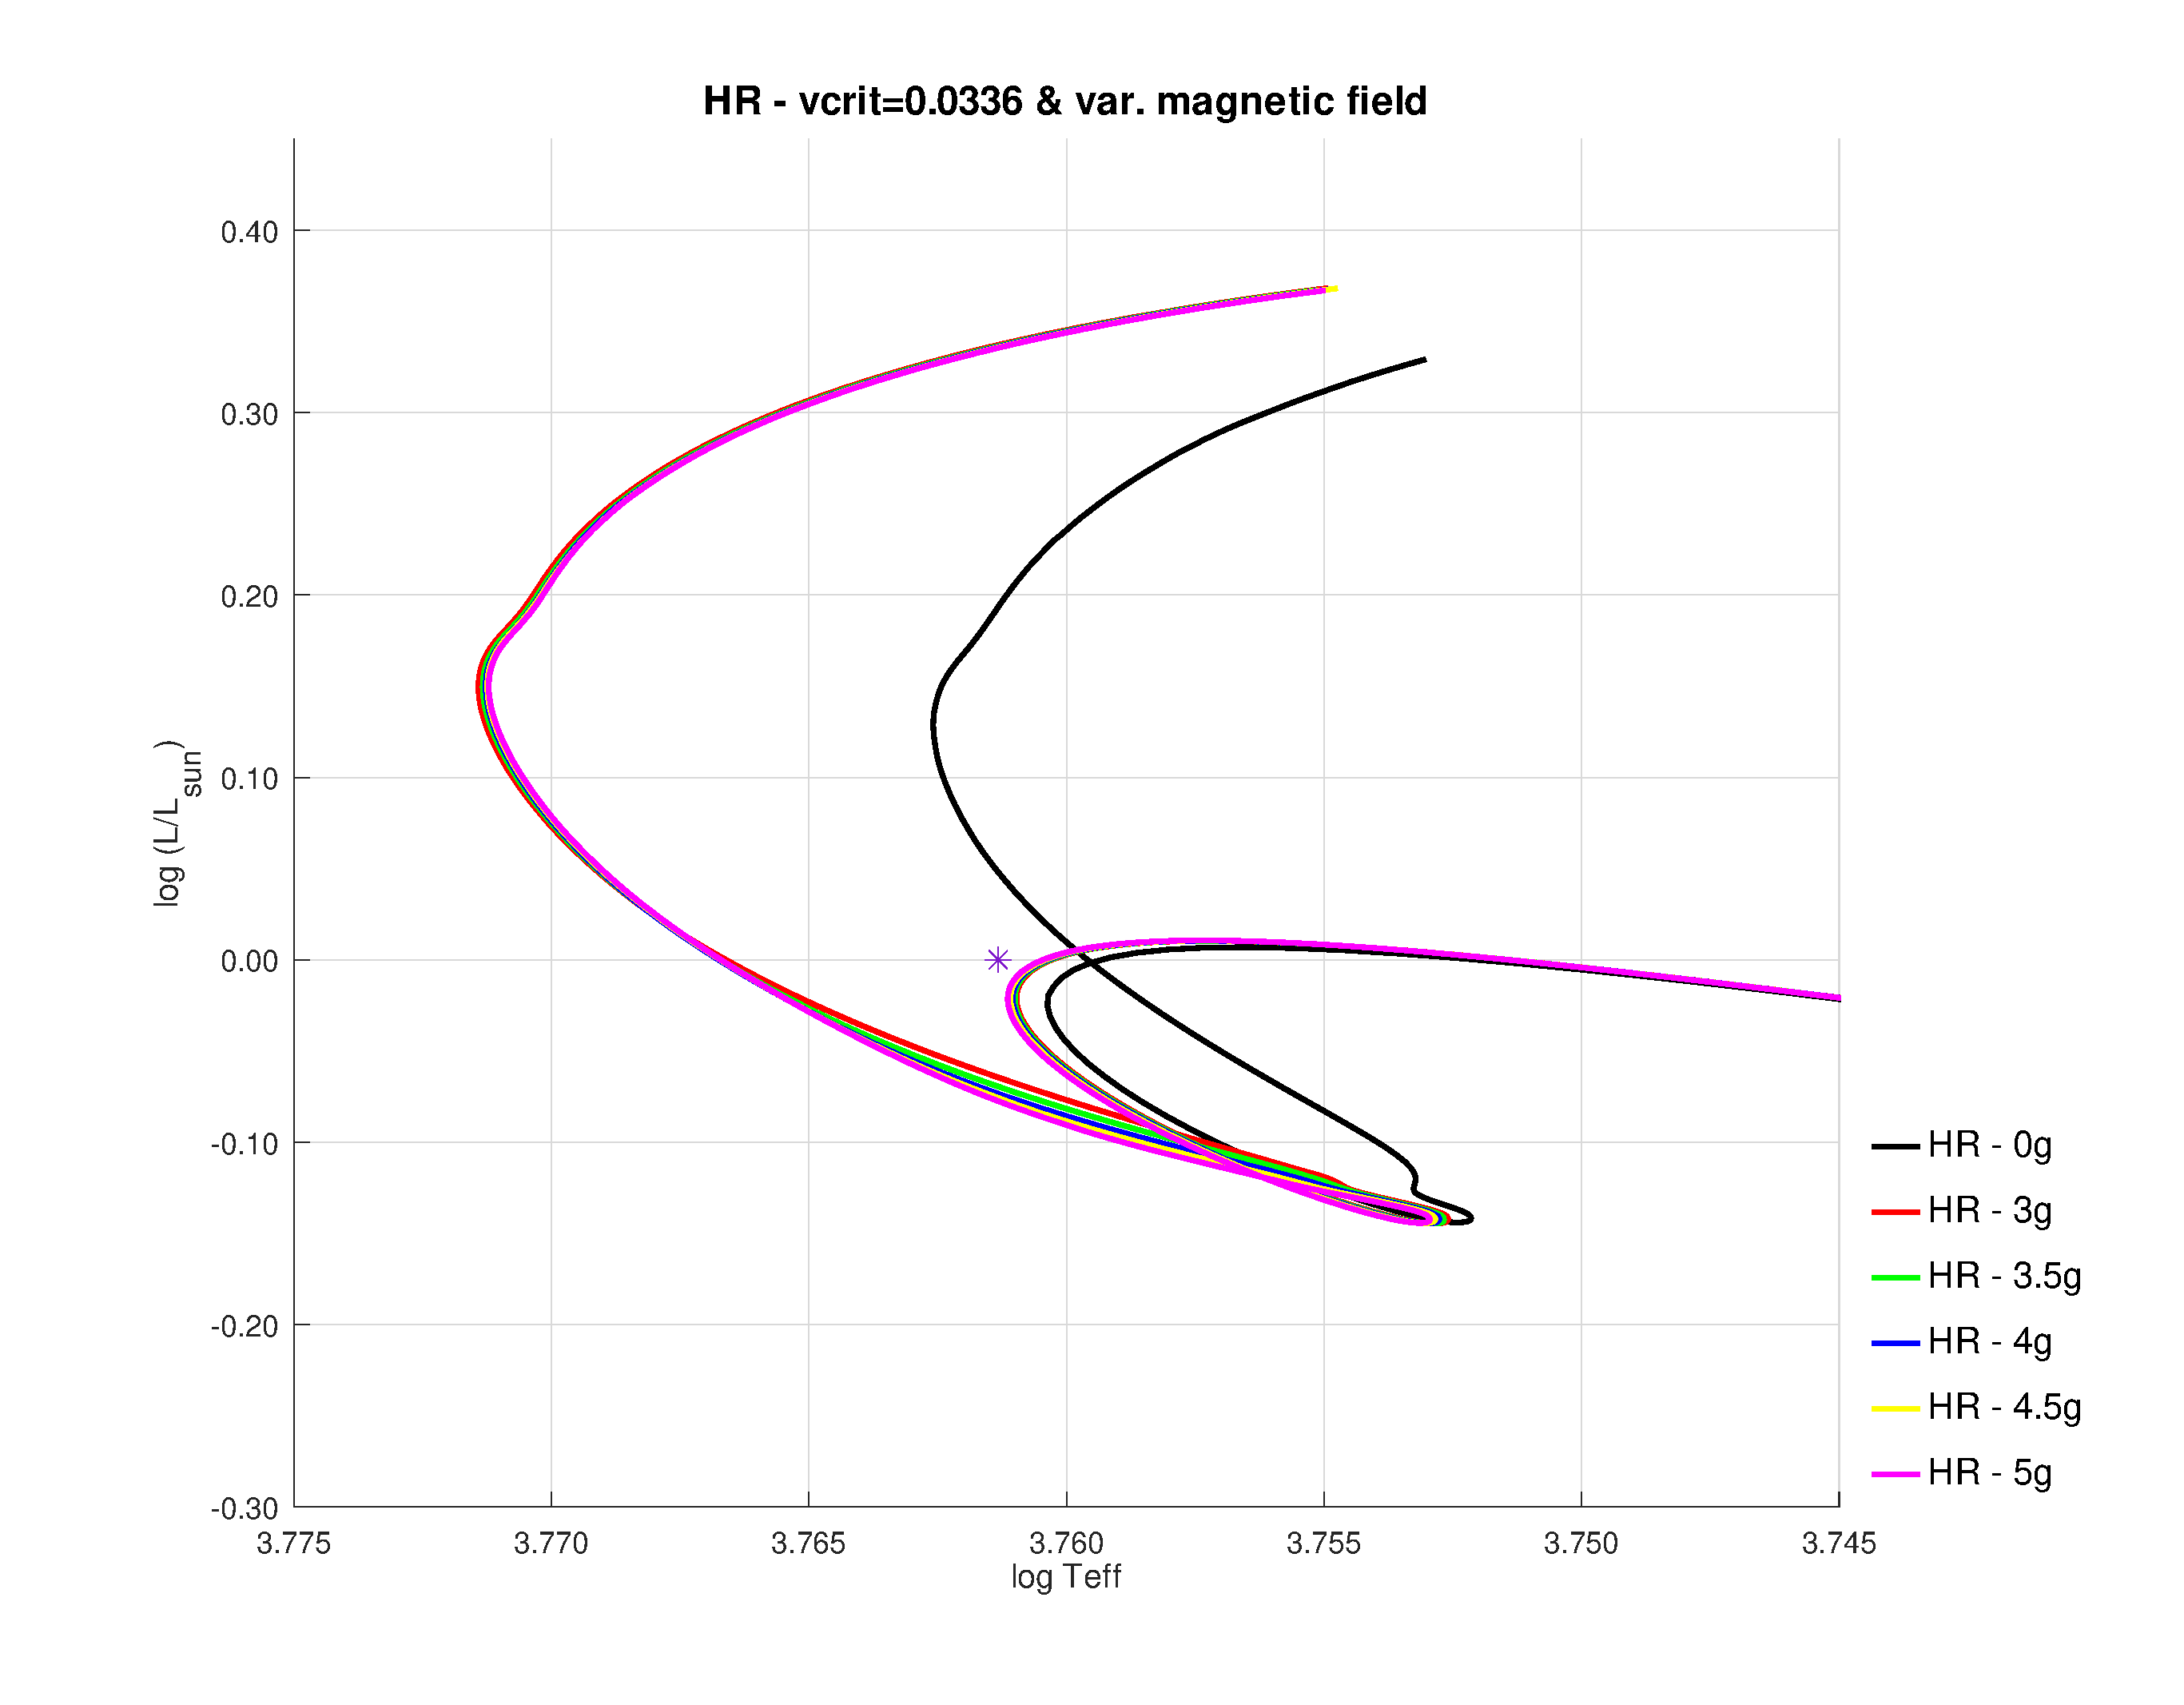
\includegraphics[trim = 30mm 15mm 15mm 15mm, clip,width=\columnwidth]{figures/hr_vc_0336_var_g_z1.eps}
    \caption{Similar to figure (\ref{fig:hr_var_vel_0g}) but now showing in detail the effects of magnetic braking on the evolutionary tracks for different magnetic field strengths and $\Omega / \Omega_{crit}=0.0336$. The presence of a magnetic field produces hotter stars due to the influence of the magnetic braking on the rotational velocity of the star.}
    \label{hr_vc_0336_var_g_z1}
\end{figure}



As described in section \ref{mod_ang_vel_ang_mom}, the MB routine distributes the total amount of AML calculated according to equation (\ref{eq:k_jdot}) among the different layers that compose it. In figure (\ref{fig:cz_vc_028_var_b}) we can observe the evolution of the most external CZ normalized with respect to the radius of the star. In accordance with the established models of stellar evolution, in a solar-type star the CZ covers practically all of it for a large part of the PMS. As it approaches the ZAMS, the CZ is decreasing as a consequence of the appearance of a radiative core and maintains an approximately constant radius until the final stage of the MS. In this point it increases significantly as a response to the generalized expansion of the star's radius. Regarding the effect of MB on the size of the CZ, we observe that as the intensity of the magnetic field increases, the size of the CZ decreases. According to \citet{Jeffries2004} this direct consequence is expected because the magnetic fields in the CZ raise the adiabatic temperature gradient and accelerate the formation of a radiative core. This radiative core pushes outward to include a rapidly increasing fraction of the stellar mass, making that the temperature at the CZ base drops below $T_{Li}$. This effect is most evident during MS (figure (\ref{fig:cz_vc_028_var_b_z1})). The decrease in the size of the CZ is in line with the fact that less Li is destroyed by causing less star material to reach areas with temperatures above $T_{Li}$.\par

Similar to the evolution of the $\Omega$ towards the end of the MS, we observe that the size of the CZ also shows a series of ups and downs. Again we think that this effect is a direct consequence of the temporal resolution used by MESA in the stellar evolution equations. The specific origin of these fluctuations is a subject that we will deal with in more depth and detail in subsequent works.\par

\begin{figure}
	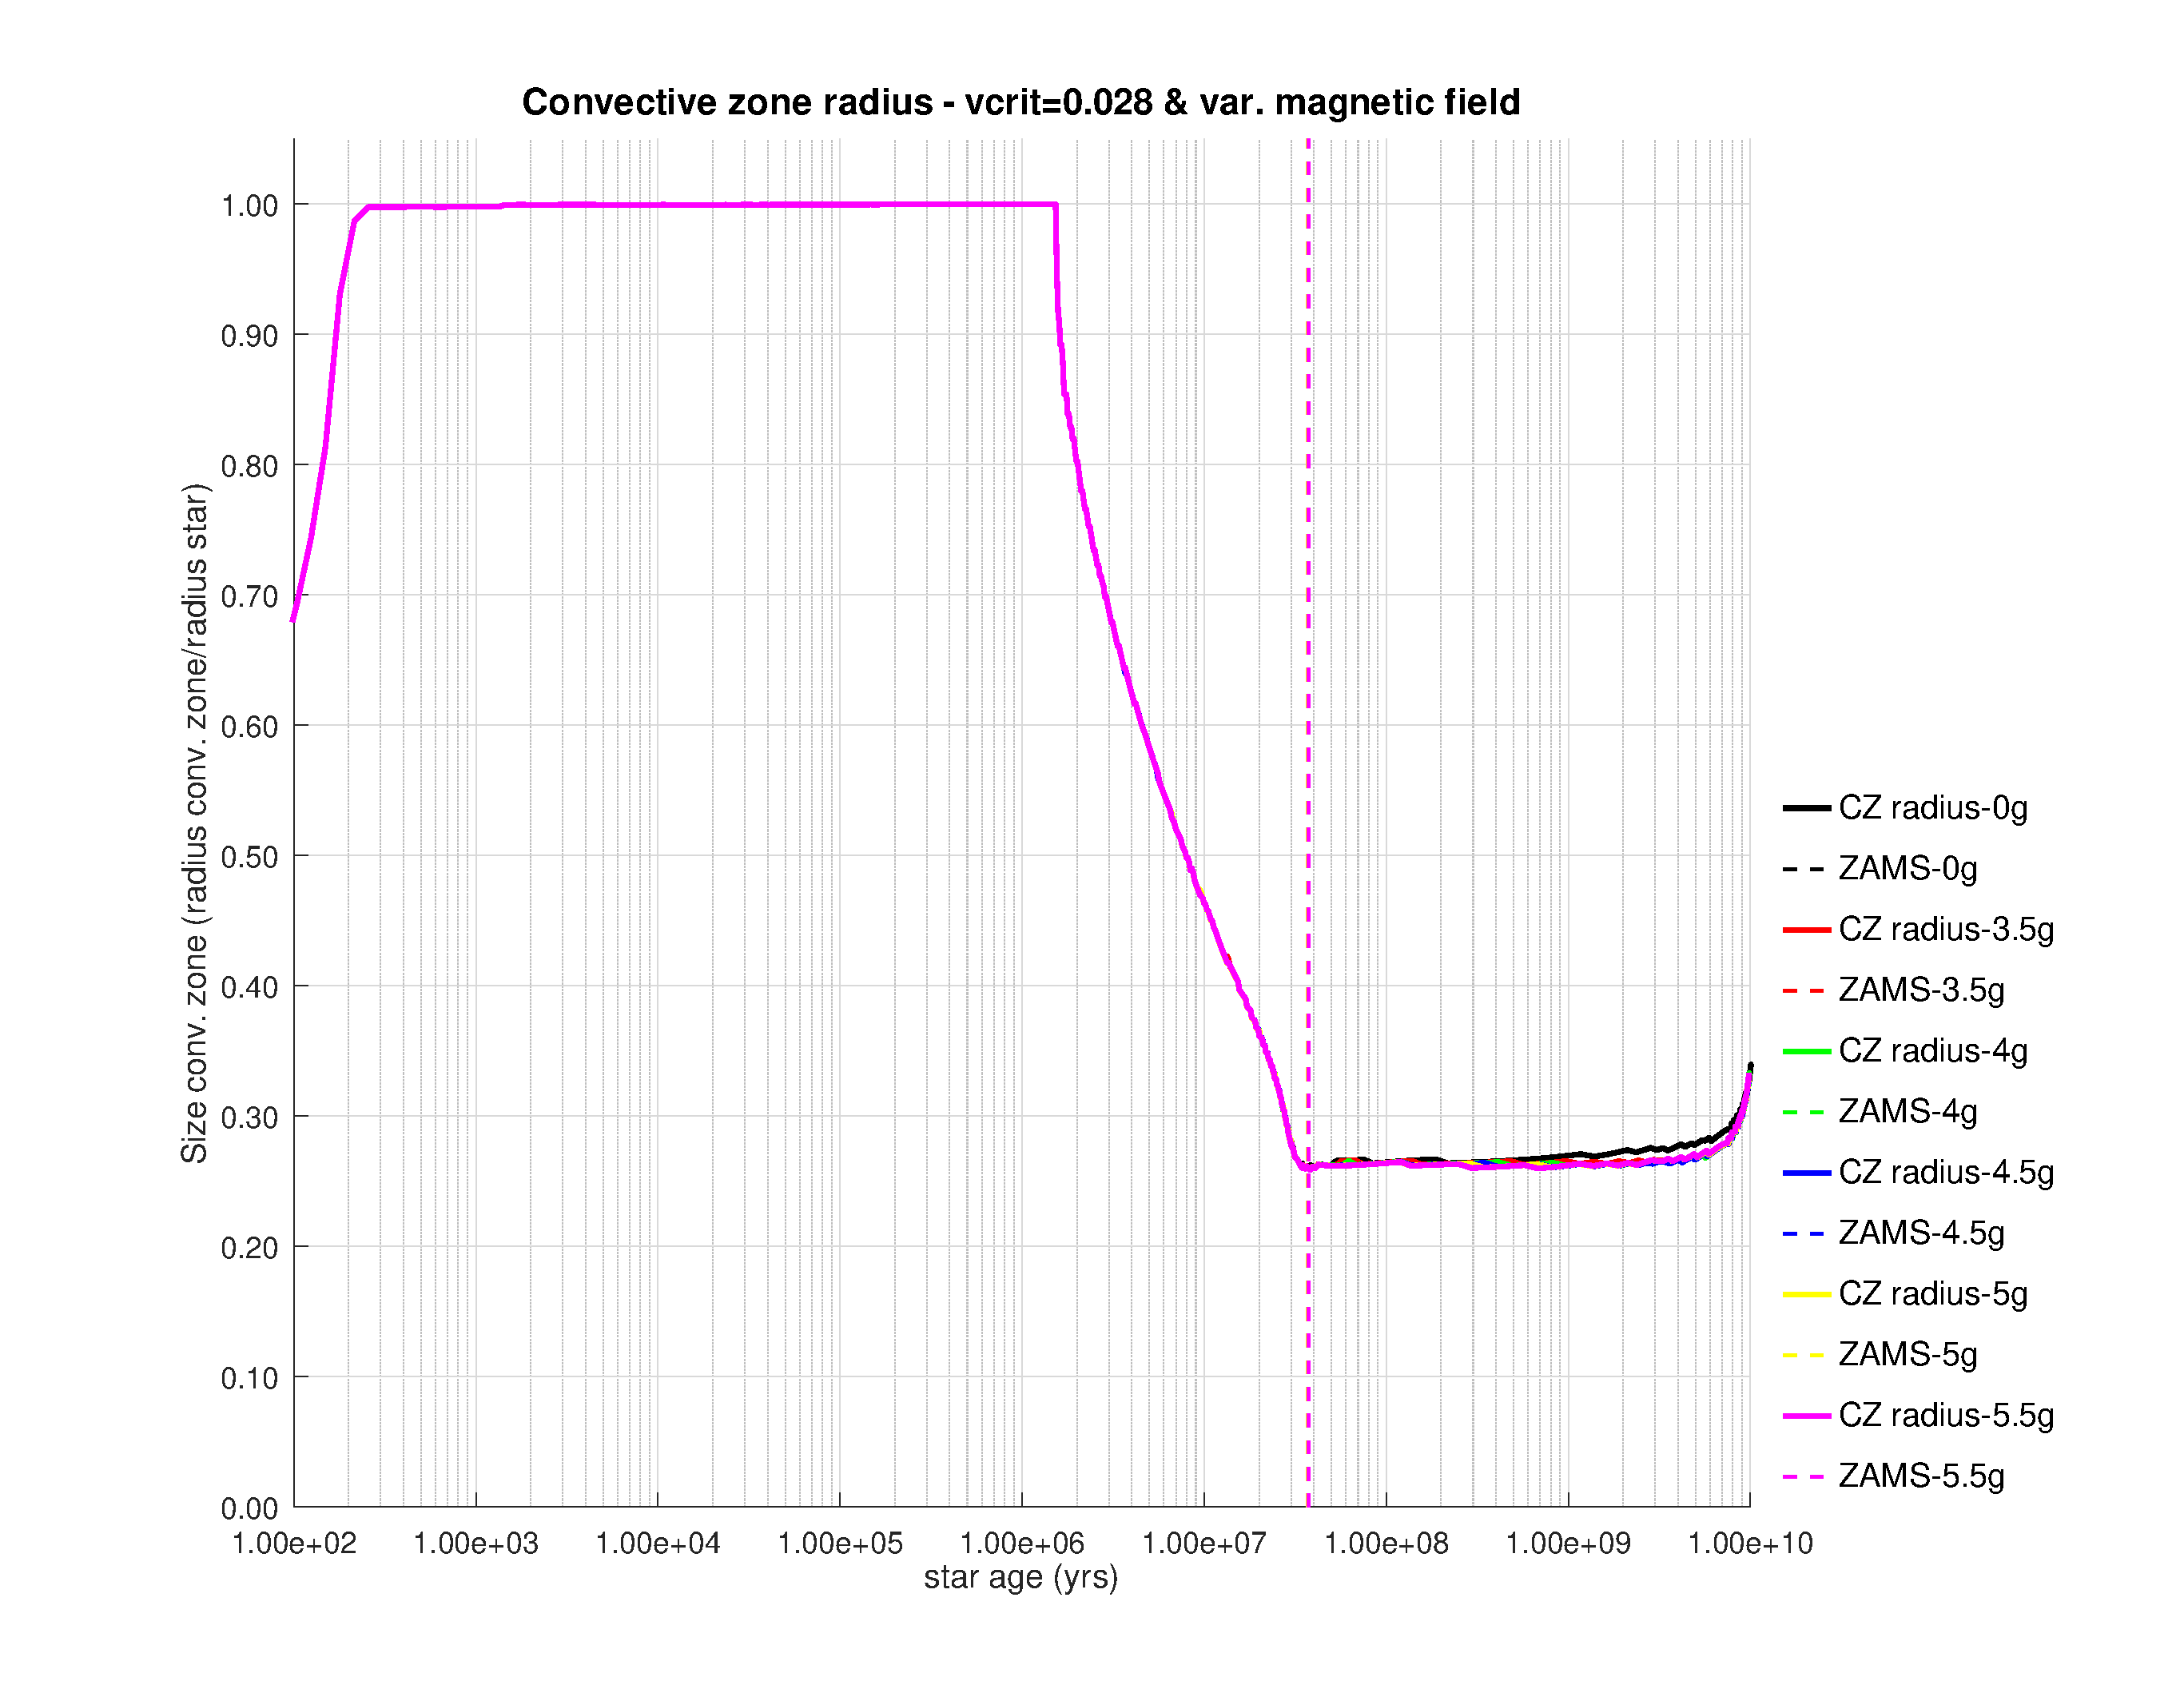
\includegraphics[trim = 30mm 15mm 20mm 15mm, clip,width=\columnwidth]{figures/cz_vc_028_var_g.eps}
    \caption{The evolution of convective zone size, as a function of time for several 1 $M_{\sun}$ models. The models include a magnetic field with an intensity of 4G and PMS rotation with $\Omega / \Omega_{crit}$ between 0.0084 and 0.0336, respectively. Additionally it's simulated the magnetic braking effect of magnetic field with an intensity of 4G.The dashed lines make reference to the ZAMS.}
    \label{fig:cz_vc_028_var_b}
\end{figure}

\begin{figure}
	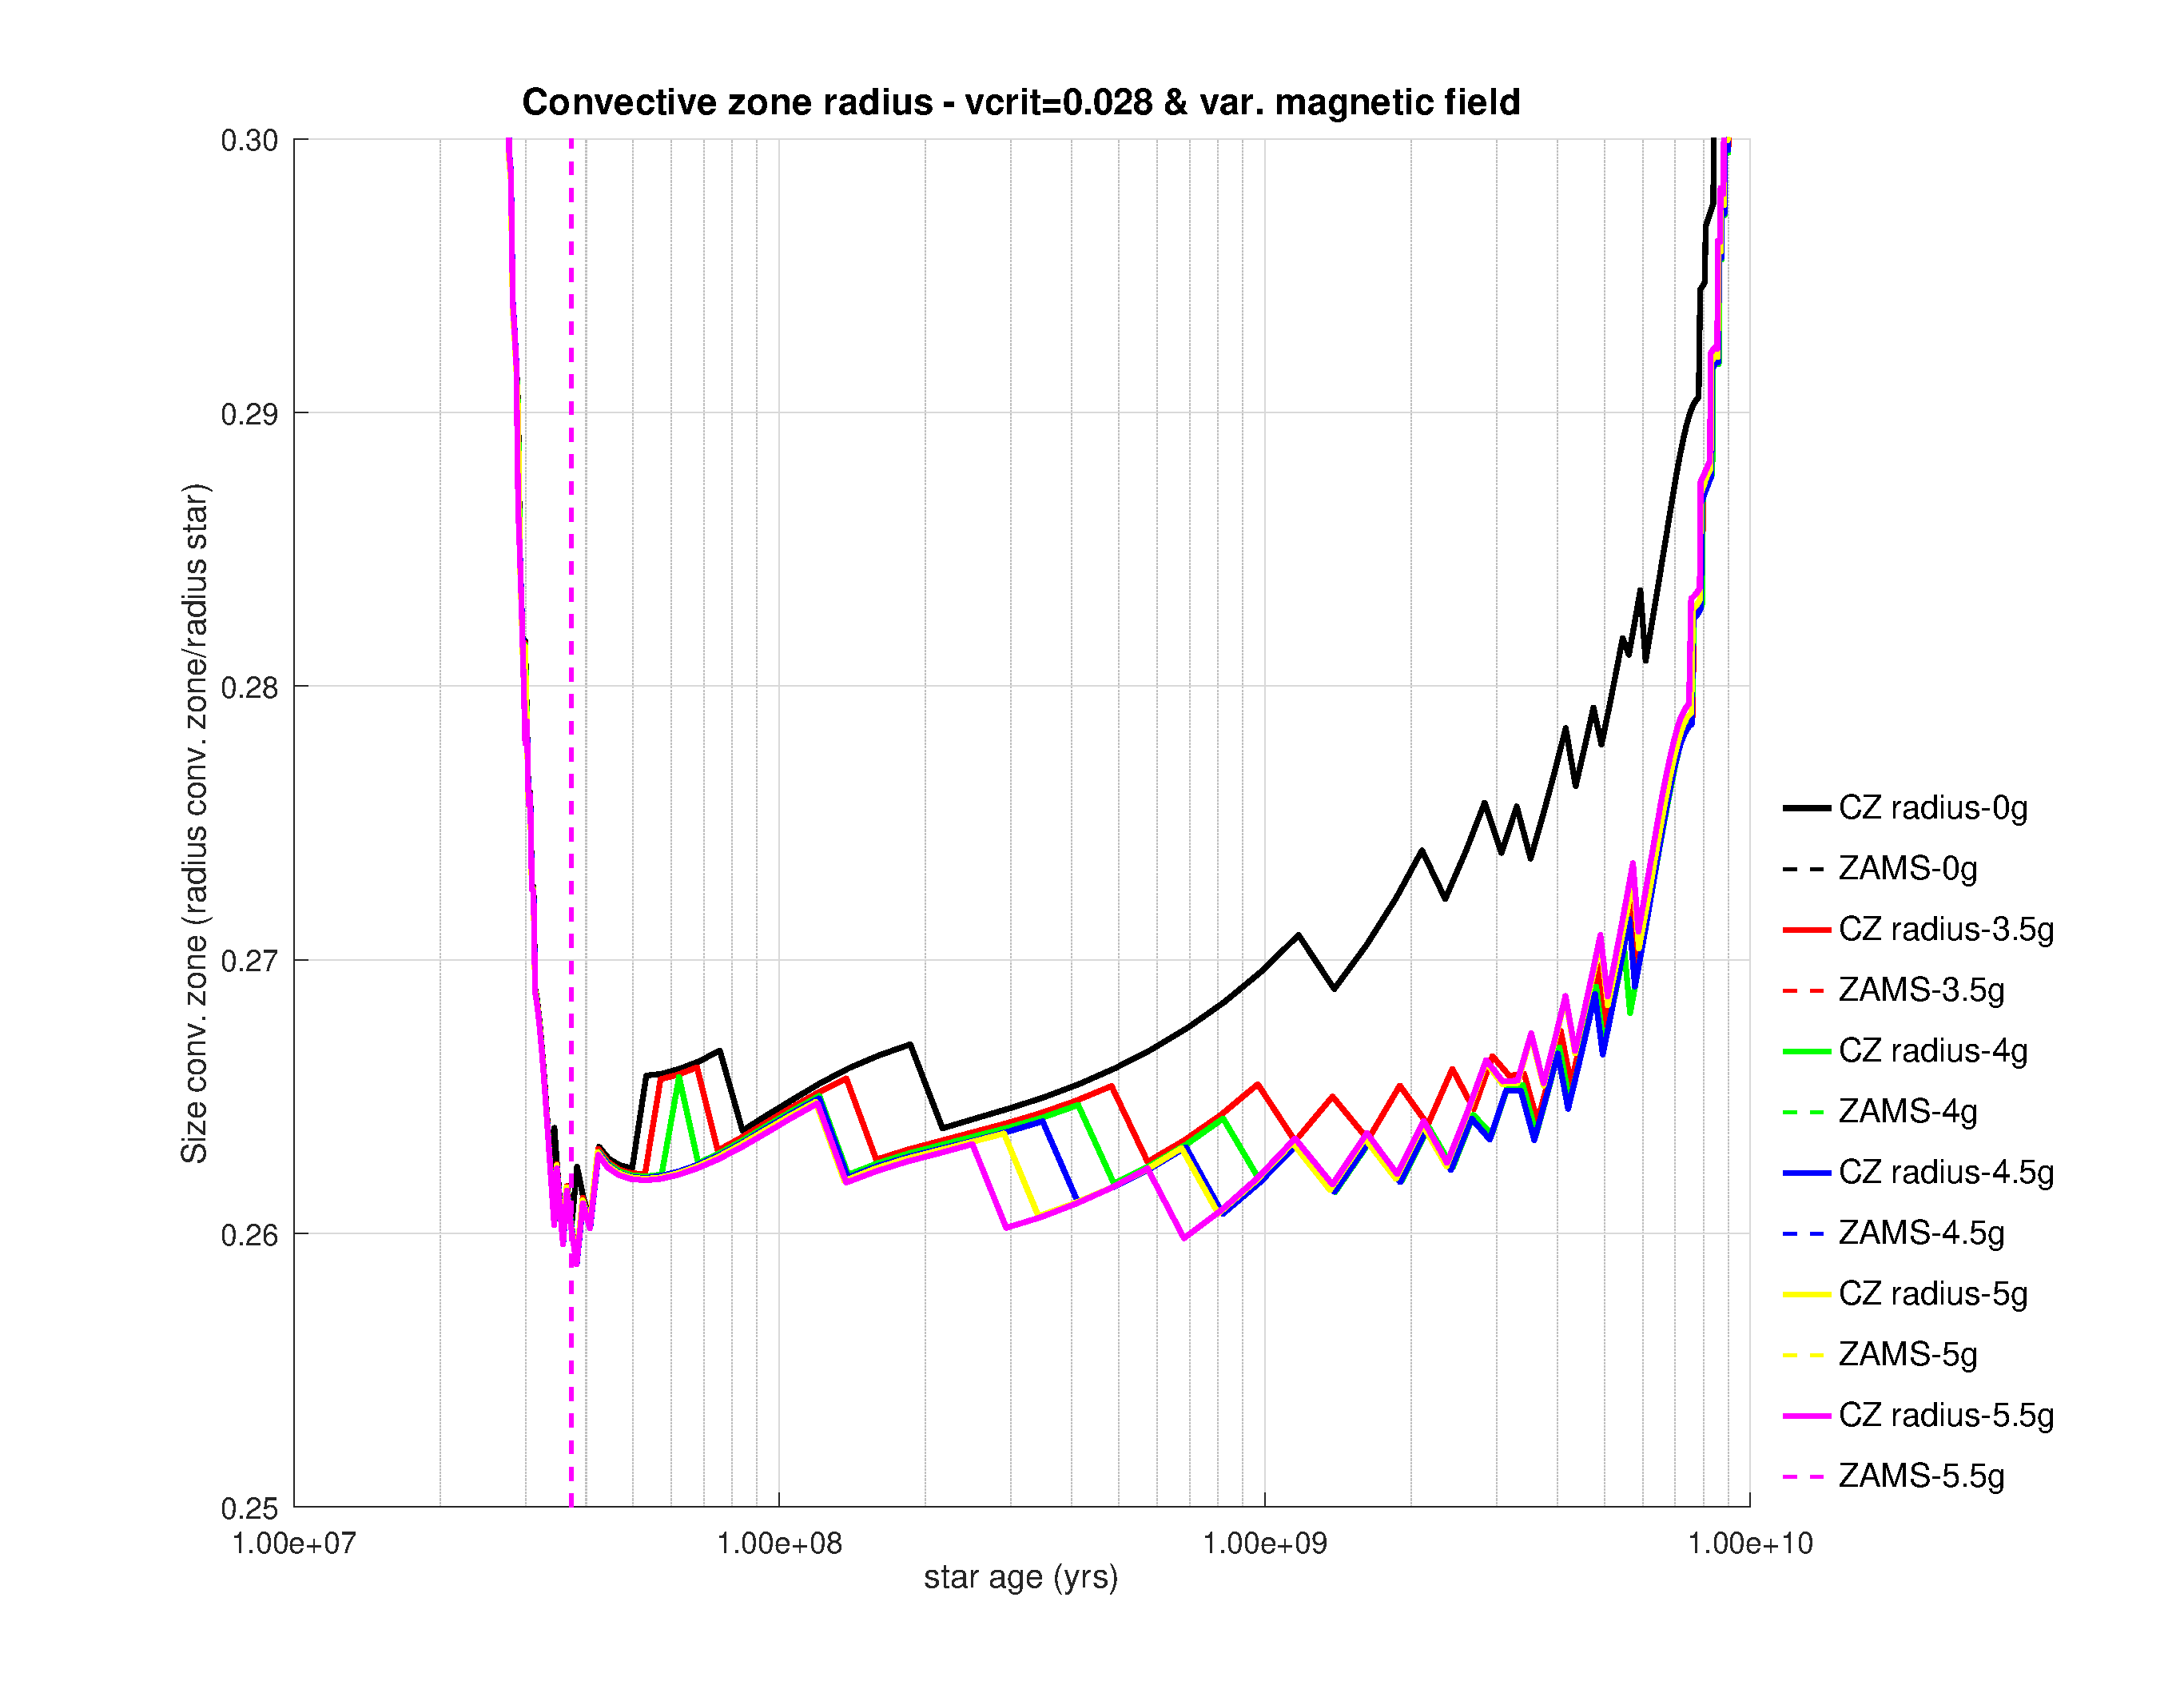
\includegraphics[trim = 30mm 15mm 20mm 15mm, clip,width=\columnwidth]{figures/cz_vc_028_var_g_z1.eps}
    \caption{Similar to figure (\ref{fig:cz_vc_028_var_b}) but now showing in detail the convection zone size from the near ZAMS till the TAMS. As the intensity of the magnetic field increases, the size of the convective zone decreases.}
    \label{fig:cz_vc_028_var_b_z1}
\end{figure}

Before ending this section we would also like to comment on the other factor that directly affects AML; the loss of mass, $\Dot{M}$. In figure (\ref{fig:mdot_vc_028_var_b}) we can see the evolution of $\Dot{M}$ during PMS and MS. In the first stages of PMS is where the greatest loss of mass is concentrated and this diminishes as it approaches the ZAMS. If we add to this scenario the fact that the star also decreases its radius during the PMS we have as result that the star increases $\Omega$ obeying the principle of conservation of AM. When reaching the ZAMS, the radius of the star remains more or less stable for much of the MS (except for its final stage) but continues to lose mass so it also increases its $\Omega$, although in a less aggressive way if we compare it with the PMS. However, as a consequence of both the appearance of the radiative core during Henyey track and the existence of a CZ (see figures (\ref{fig:mb_act_var_vel_vc_028}) \& (\ref{fig:grid_mb_act})), the MB routine is activated, causing the angular velocity of the star to begin to decrease along the entire MS. The more intense the magnetic field, the greater the braking effect.\par 

\begin{figure}
	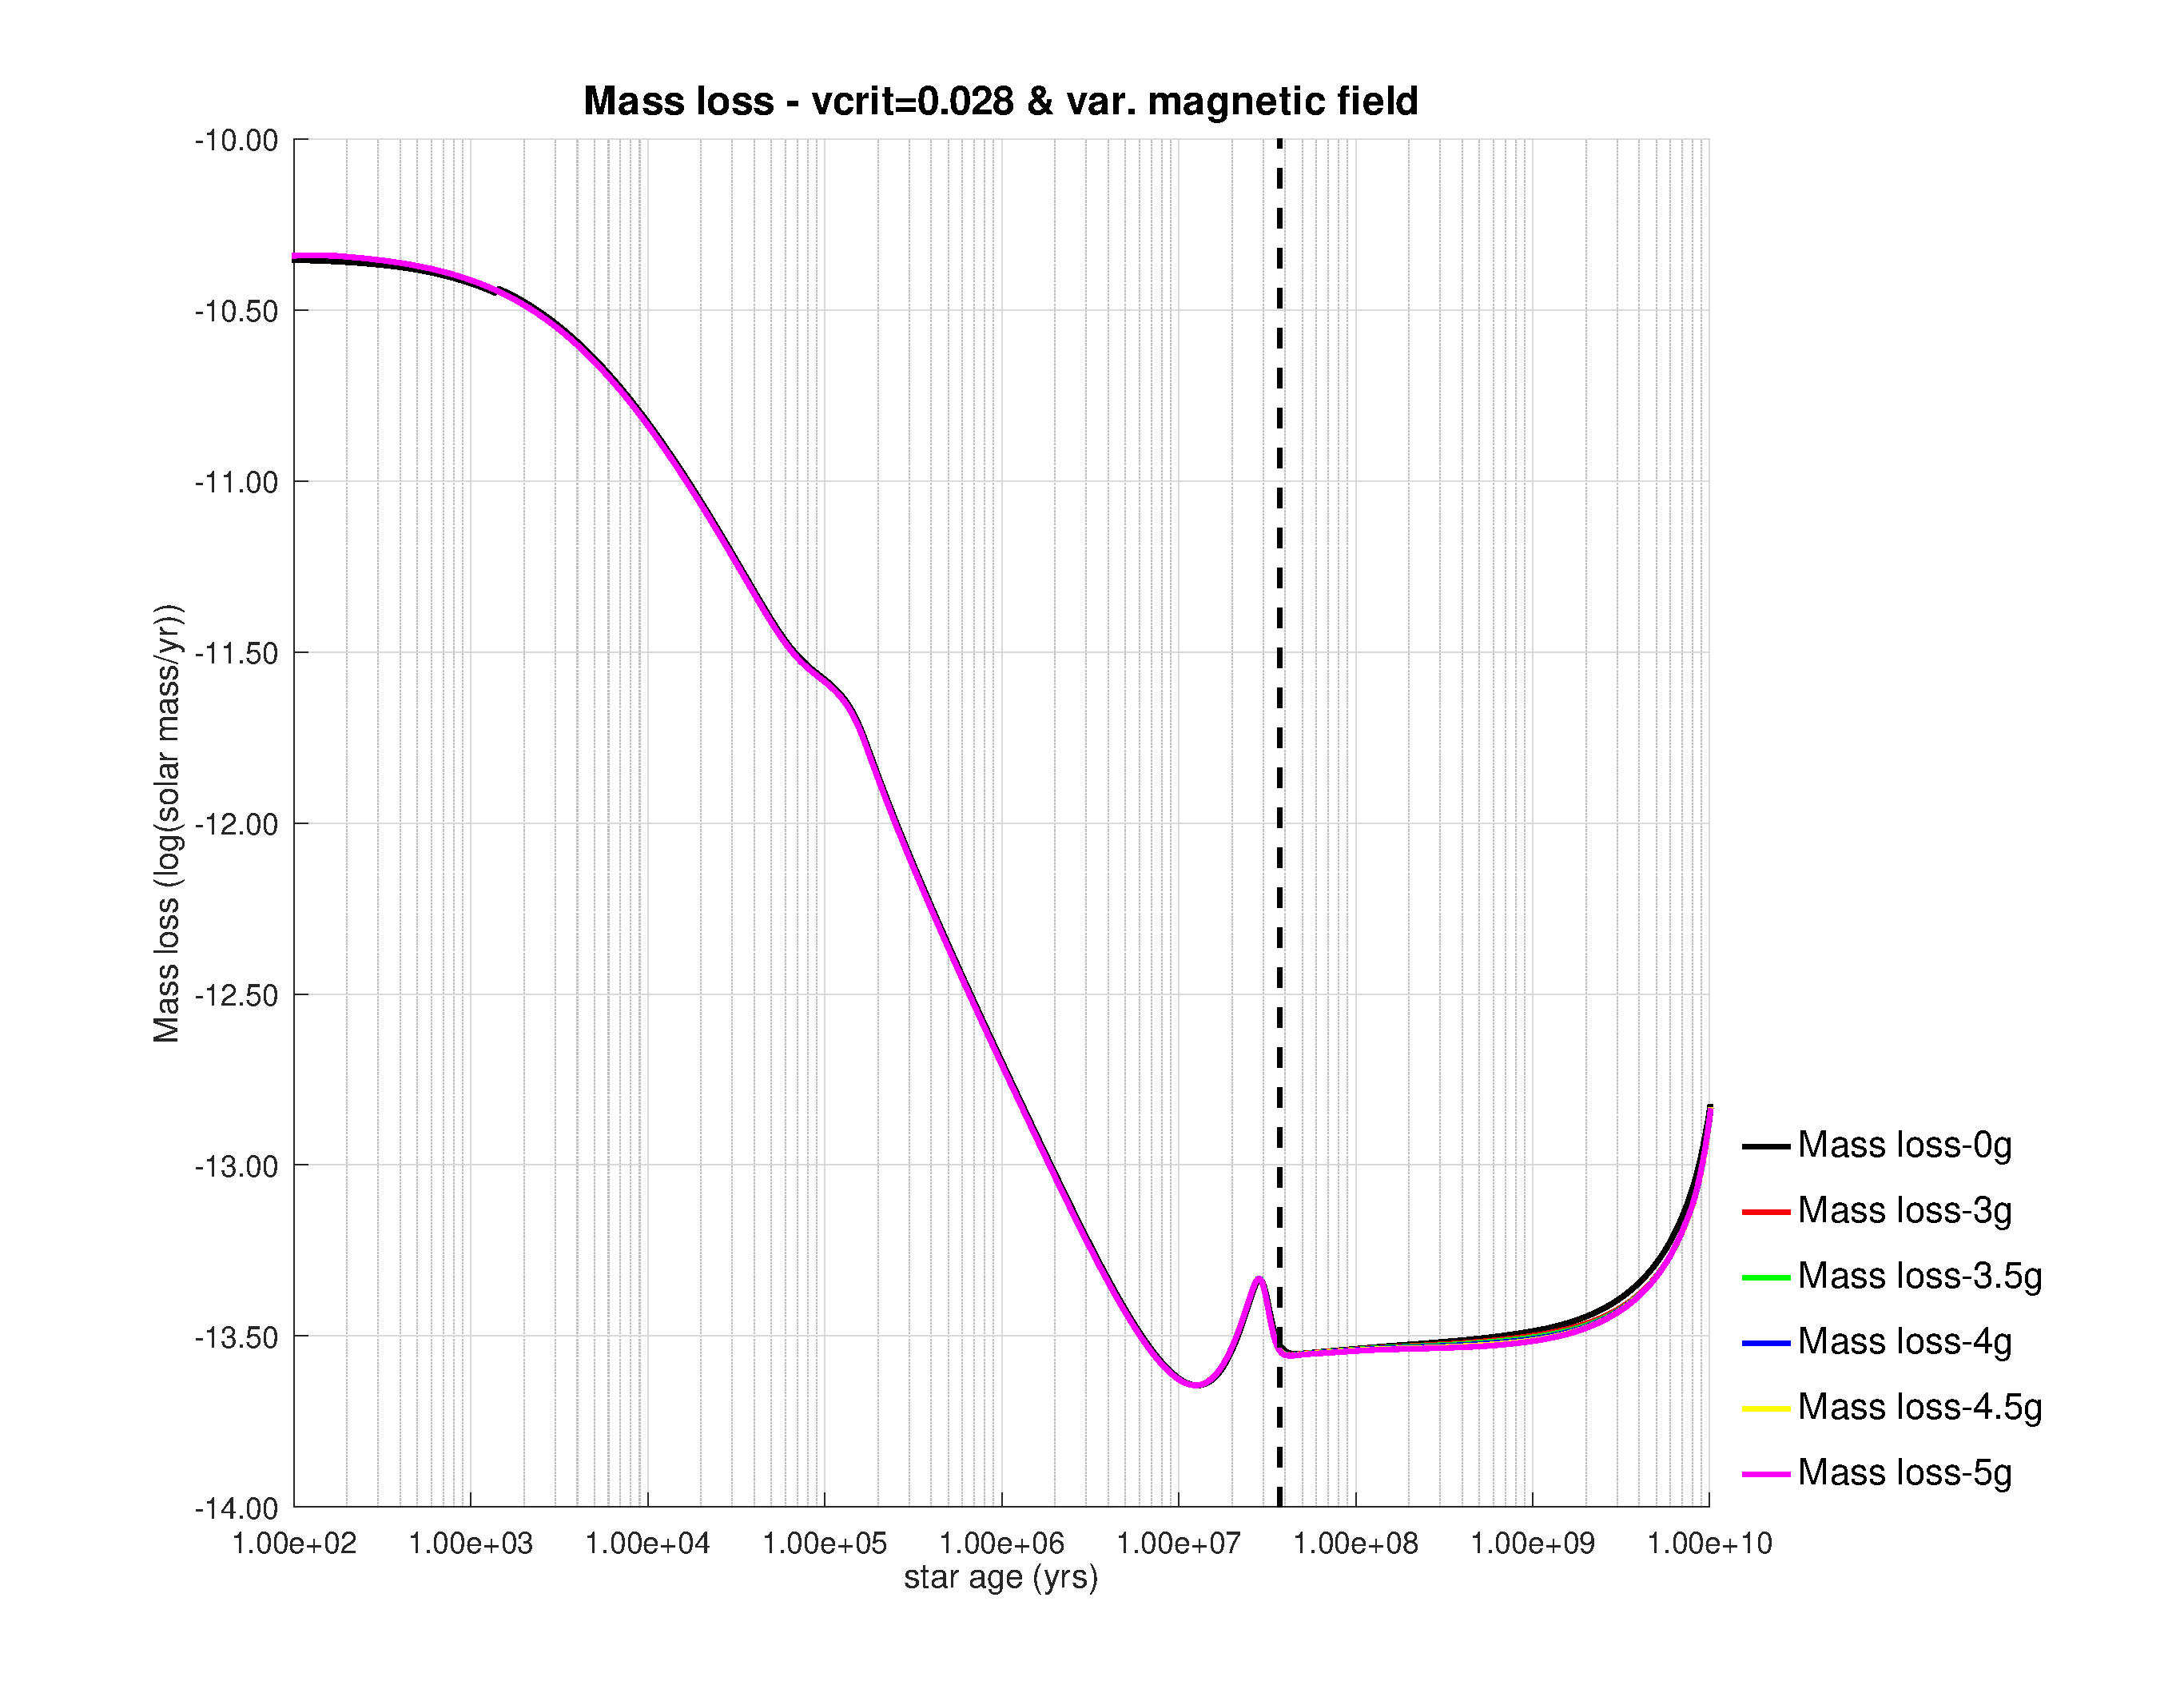
\includegraphics[trim = 30mm 15mm 20mm 15mm, clip,width=\columnwidth]{figures/mdot_vc_028_var_g.eps}
    \caption{The evolution of mass loss $\Dot{M}$ , as a function of time for several 1 $M_{\sun}$ models. The models include a variable magnetic field intensity between $0\,G$ and $5.5\,G$ and PMS rotation with $\Omega / \Omega_{crit}=0.028$. The dashed lines make reference to the ZAMS.}
    \label{fig:mdot_vc_028_var_b}
\end{figure}

\begin{figure}
	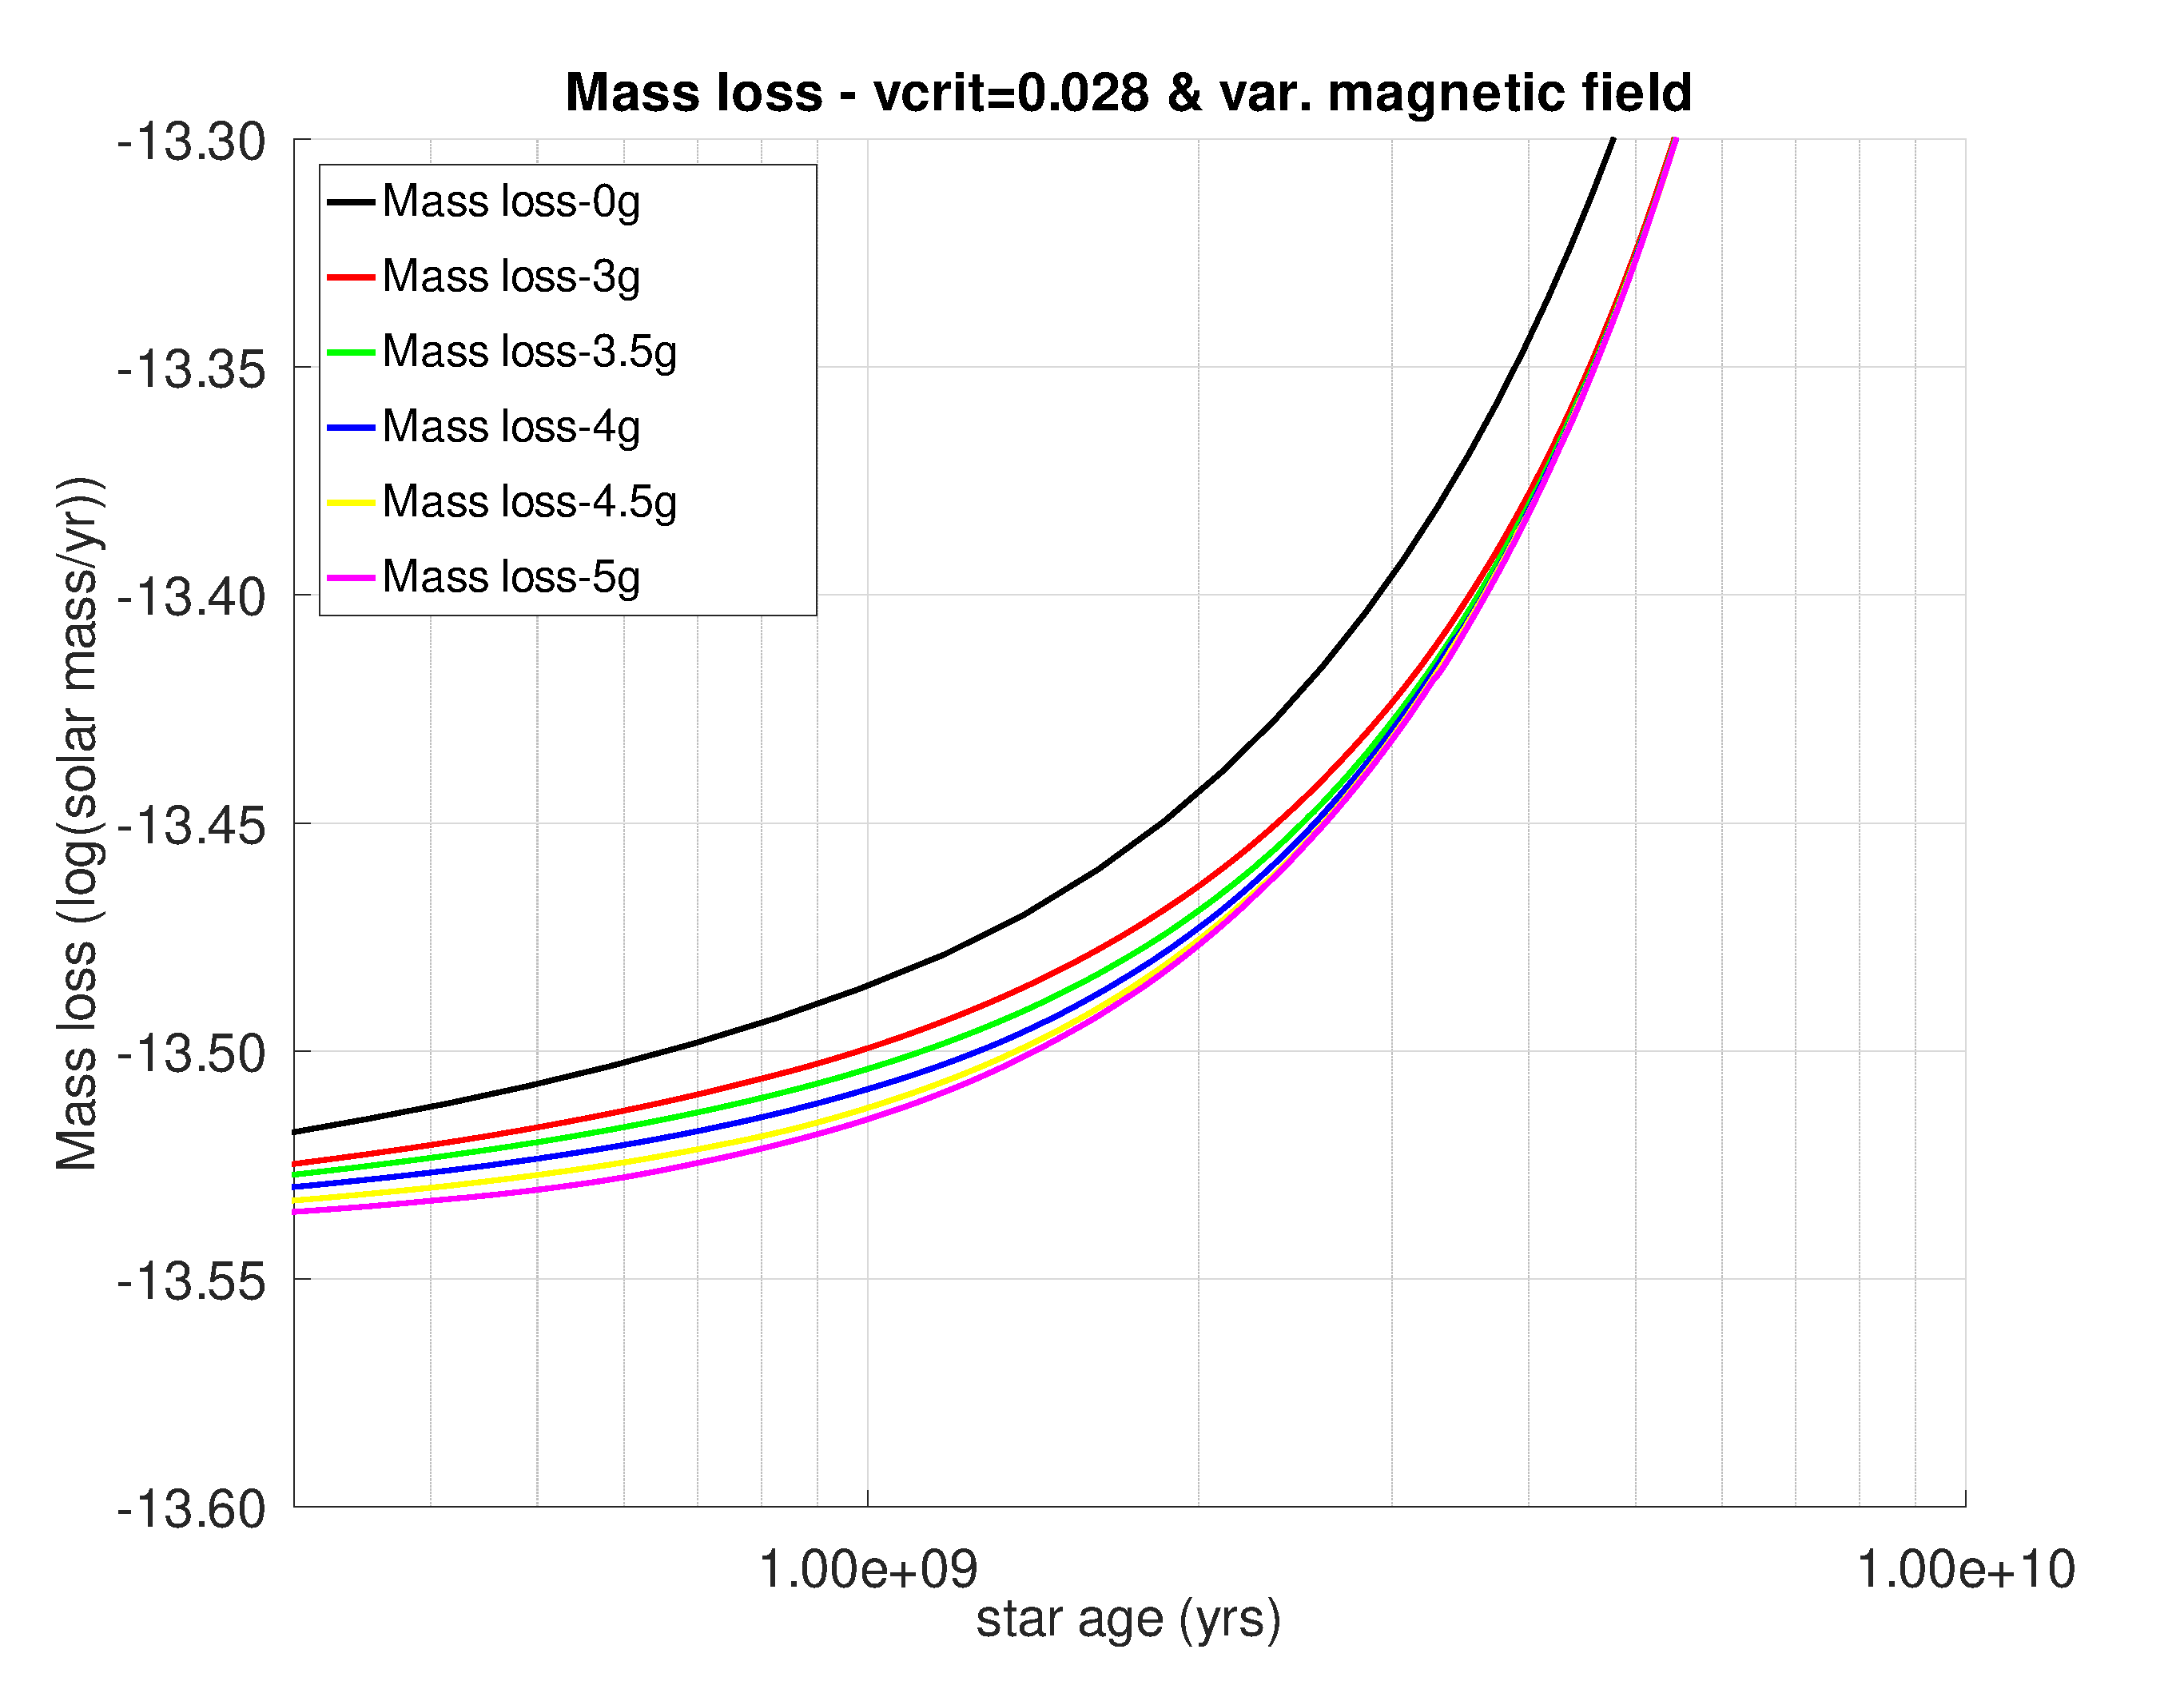
\includegraphics[trim = 30mm 15mm 20mm 15mm, clip,width=\columnwidth]{figures/mdot_vc_028_var_g_z1.eps}
    \caption{The evolution of mass loss $\Dot{M}$ as the star is approaching TAMS, as a function of time for several 1 $M_{\sun}$ models. The models include a variable magnetic field intensity between $0\,G$ and $5.5\,G$ and PMS rotation with $\Omega / \Omega_{crit}=0.028$. The stronger the magnetic field, the lower $\Dot{M}$.}
    \label{fig:mdot_vc_028_var_b_z1}
\end{figure}

\begin{figure}
	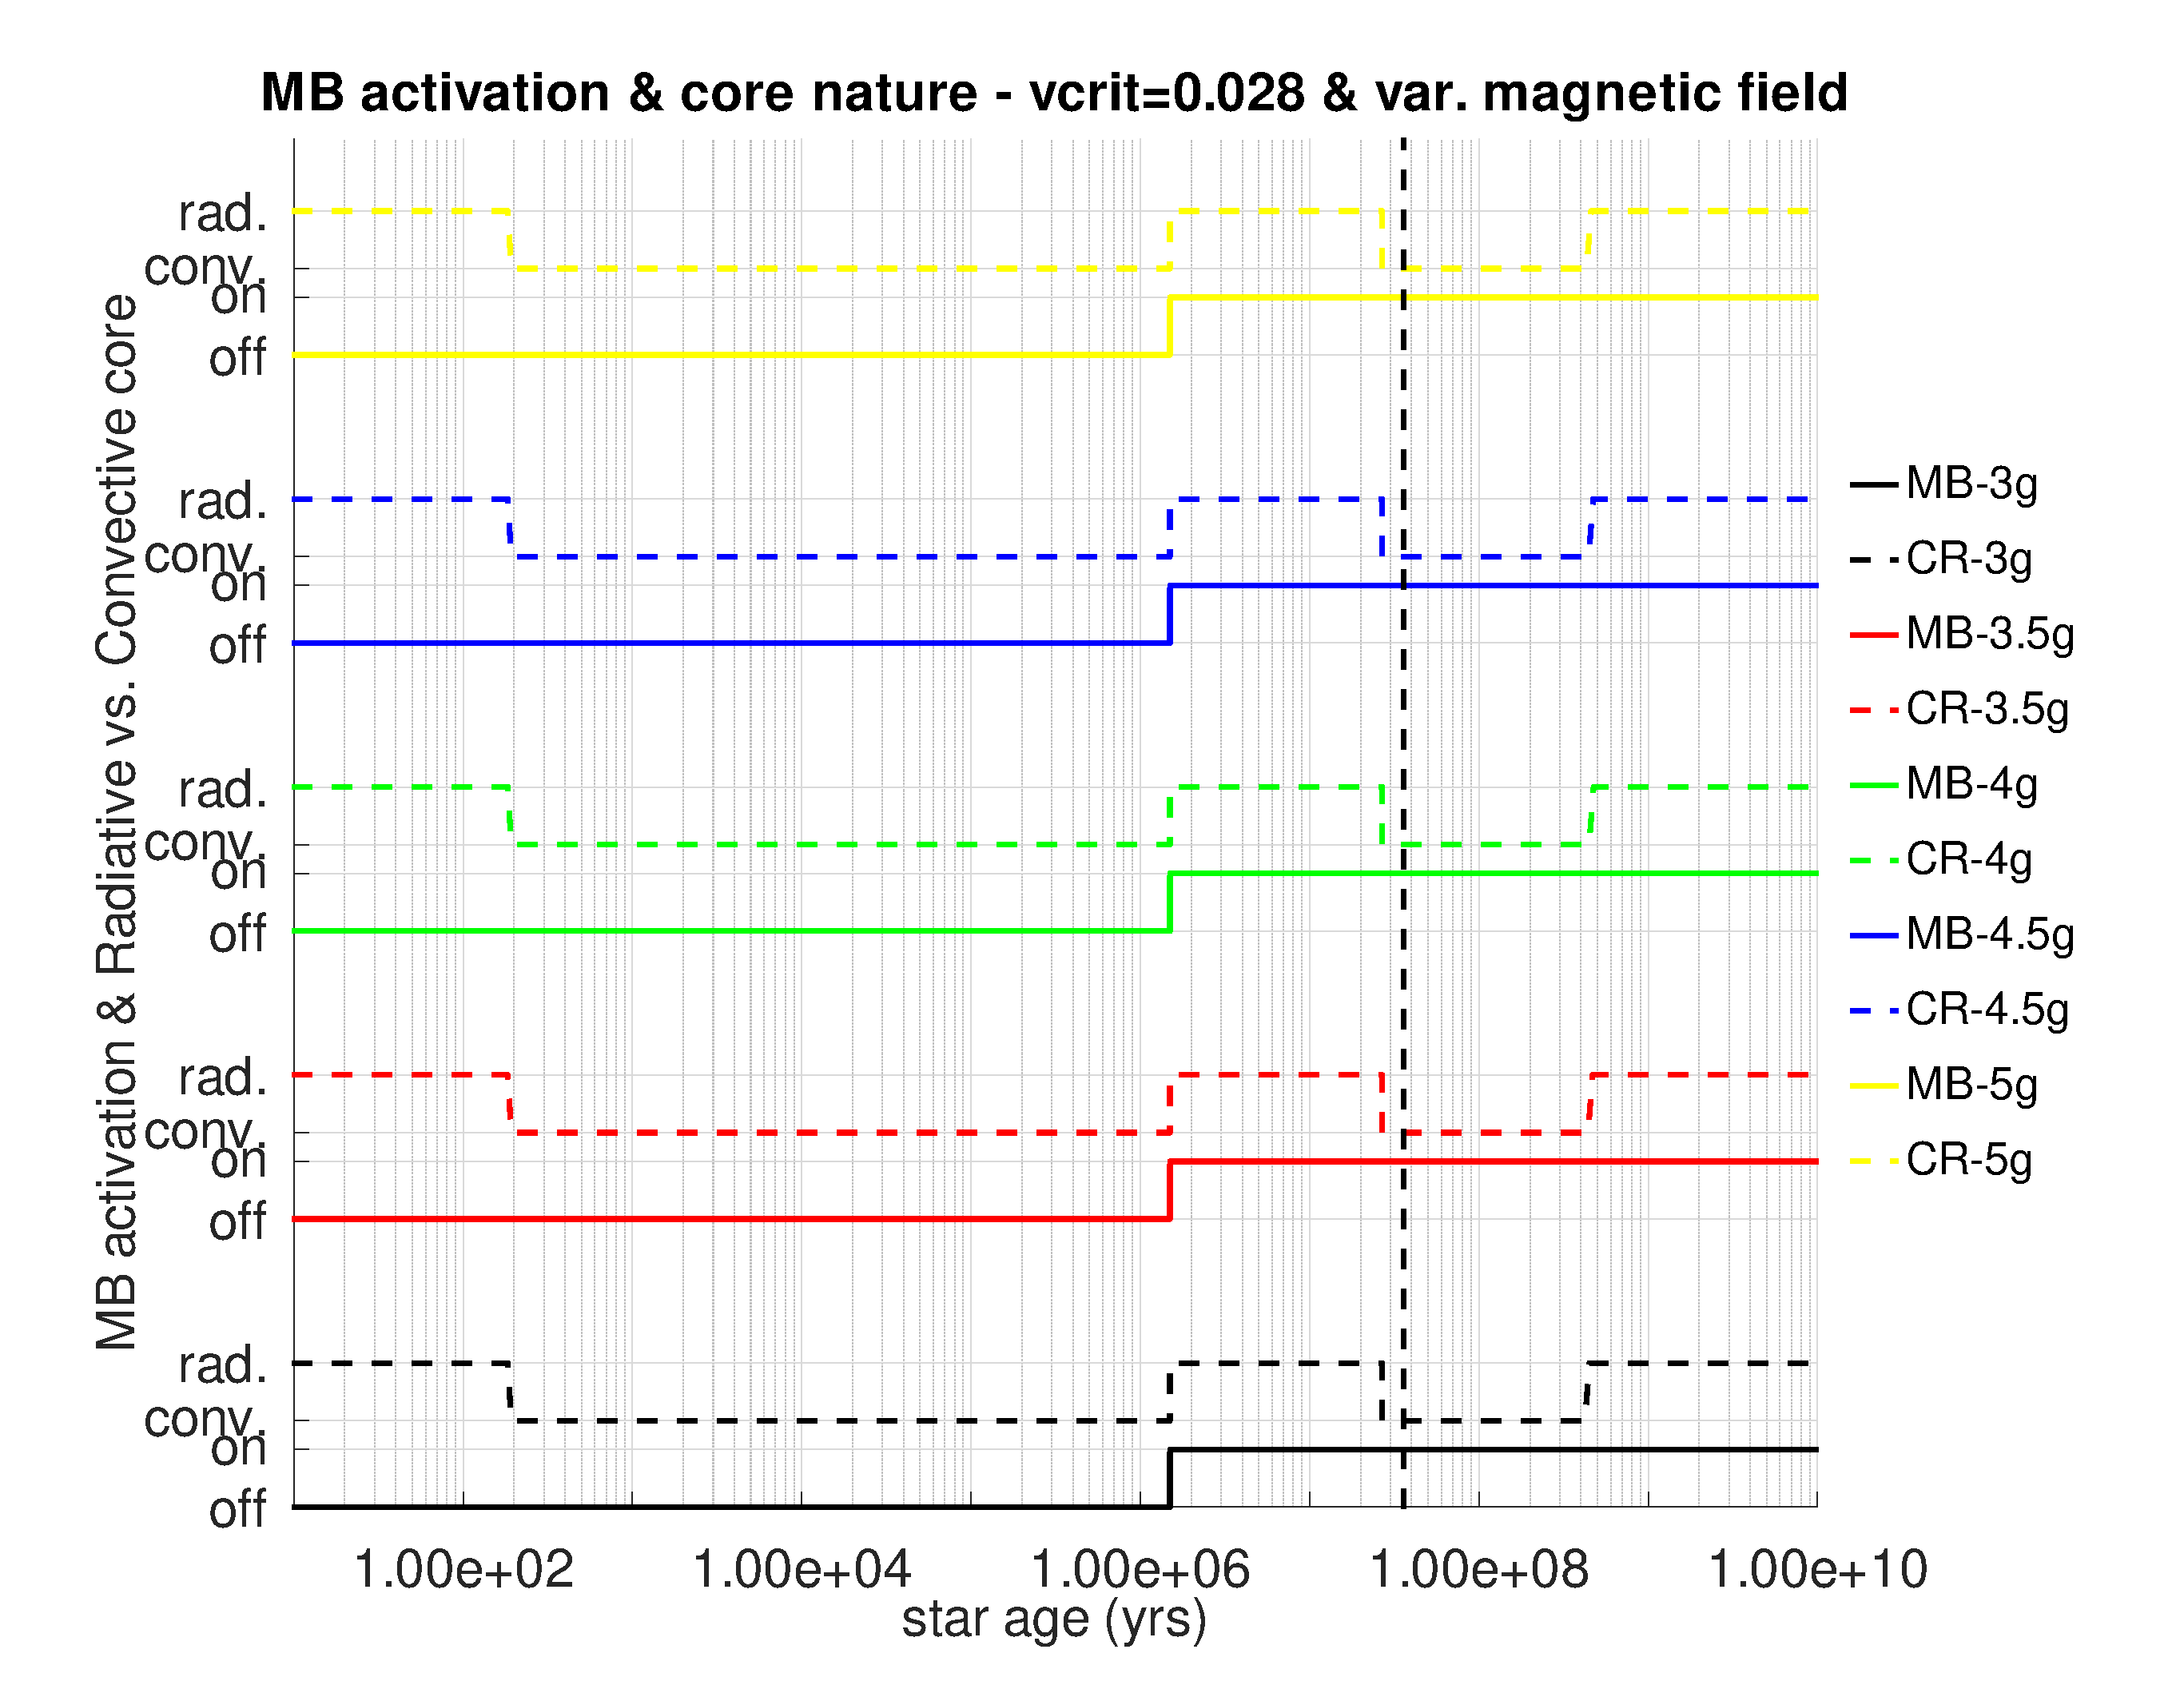
\includegraphics[trim = 30mm 15mm 15mm 15mm, clip,width=\columnwidth]{figures/mb_act_vc_028_var_g.eps}
    \caption{The activation of the magnetic braking routine as a function of the presence of a radiative core. The models include a magnetic field with an intensity ranging between $3.5\,G$ and $5.5\,G$ and PMS rotation with $\Omega / \Omega_{crit}=0.0228$. The solid lines signal the magnetic braking routine activation (on) and deactivation (off). The horizontal dashed lines inform about the star's core nature: radiative (rad) or convective (conv). By implementation decision, once the routine is activated, it remains on even if the star's core nature change to convective. The vertical dashed lines make reference to the ZAMS.}
    \label{fig:mb_act_var_vel_vc_028}
\end{figure}


\section{Conclusions and future works} \label{sec_4}
Throughout this work we are confident that we have demonstrated that both rotation and MB induced effects must be taken into account in the theoretical models for a proper understanding and modelling of the evolution of stars. The latter is of major importance both for the transport of AM and for the transport of chemical elements. We are also well aware that we are still far from understanding the exact physical mechanisms that govern these processes, so it is necessary to continue to delve into these areas of study. Particularly the study of the evolution of the magnetic fields during the PMS and MS and their impact on AML. Future and improved implementations of our routine will be made to study the results on tracks, surface Li composition, rotation, etc... It is likely that in a rotating star model simulated with MB from the beginning, the differential rotation is very much reduced and therefore Li abundances observed in young stars could be properly explained. It is equally important to understand better the general role of mass loss in AML and mostly in cooler, low-mass stars. Nowadays it's challenging to determine the terminal velocity of the stellar wind for this type of stars which, as documented previously, plays a key role on the AML.\par

We emphasize as well that our models fail to match the observed solar Li abundance and $\Omega$. We cannot, therefore, ascertain to have correctly modeled the rotational history of the Sun. In addition, we cannot (yet) properly explain the ups and downs observed in the $\Omega$ at the end of the MS. Therefore, in view of these shortcomings in our models, we must analyse the results obtained with caution and not draw any premature conclusions. Having said that, we are convinced that our research is on the right track and we do believe that the following conclusions, based on the results described in previous sections, have been sufficiently supported in the course of this work:
\begin{enumerate}
    \item Inclusion of the magnetic field leads to cooler models and lower Li depletions in the MS.
    \item A combination of rotation during the PMS and MB effect during MS produces different, potentially more promising behavior than those produced by standard models.
    \item $T_{eff}$ from standard evolutionary tracks represent upper limits since these models do not take into consideration the magnetic braking effect.
    \item The convective zone extension decreases when the intensity of the magnetic field increases.
    \item MB during PMS seems to be also required for explaining Li abundances in young clusters.
\end{enumerate}

In the near future, with the new version of our code including magnetic field evolution in MESA, we will focus our efforts on understanding how magnetic fields are linked to rotation, how their topologies are and how they evolves in time in order to go beyond the treatment on the MB routine that has been done in this work.\par




\begin{figure*}
    \centering
    \begin{subfigure}[h]{0.47\textwidth}
    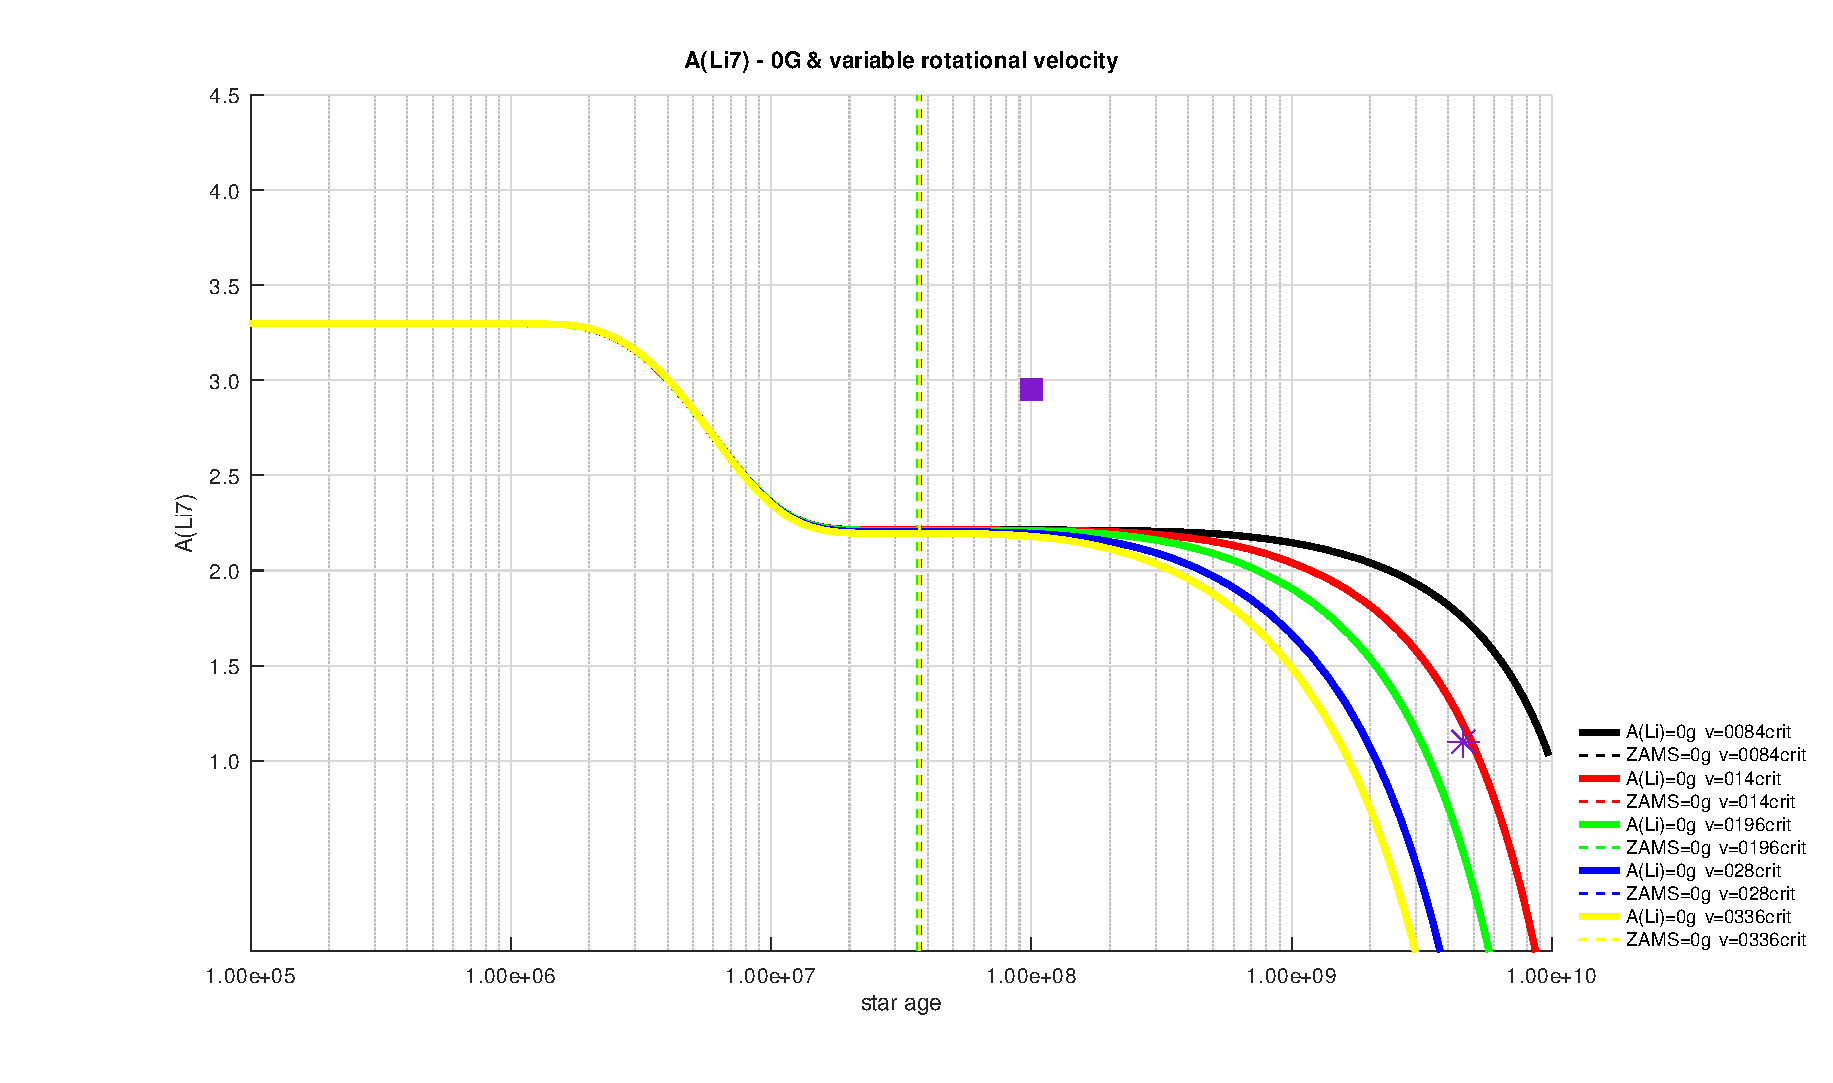
\includegraphics[trim = 40mm 15mm 20mm 15mm, clip,width=\textwidth]{figures/li_var_vel_0_0g.eps}
    \label{fig:subim1}
    \end{subfigure}
    \begin{subfigure}[h]{0.47\textwidth}
    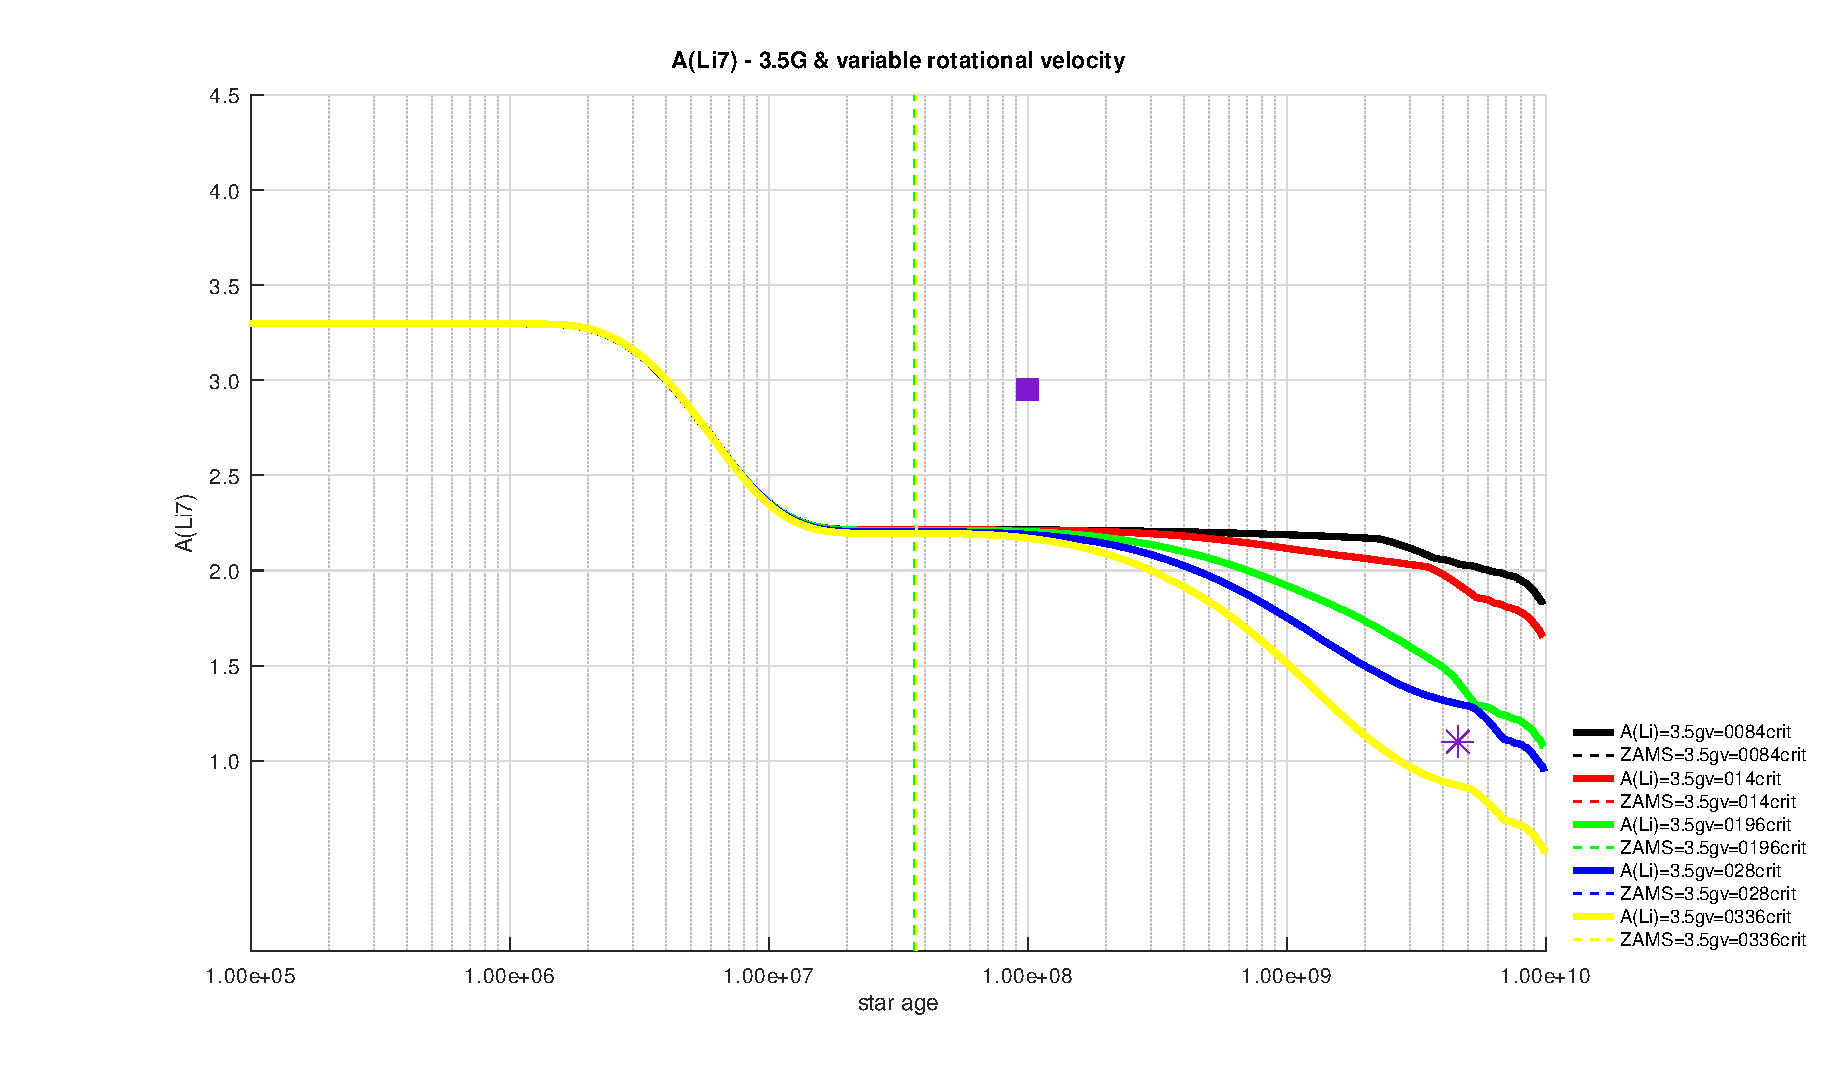
\includegraphics[trim = 40mm 15mm 20mm 15mm, clip,width=\textwidth]{figures/li_var_vel_3_5g.eps}
    \label{fig:subim2}
    \end{subfigure}
    
    \begin{subfigure}[h]{0.47\textwidth}
    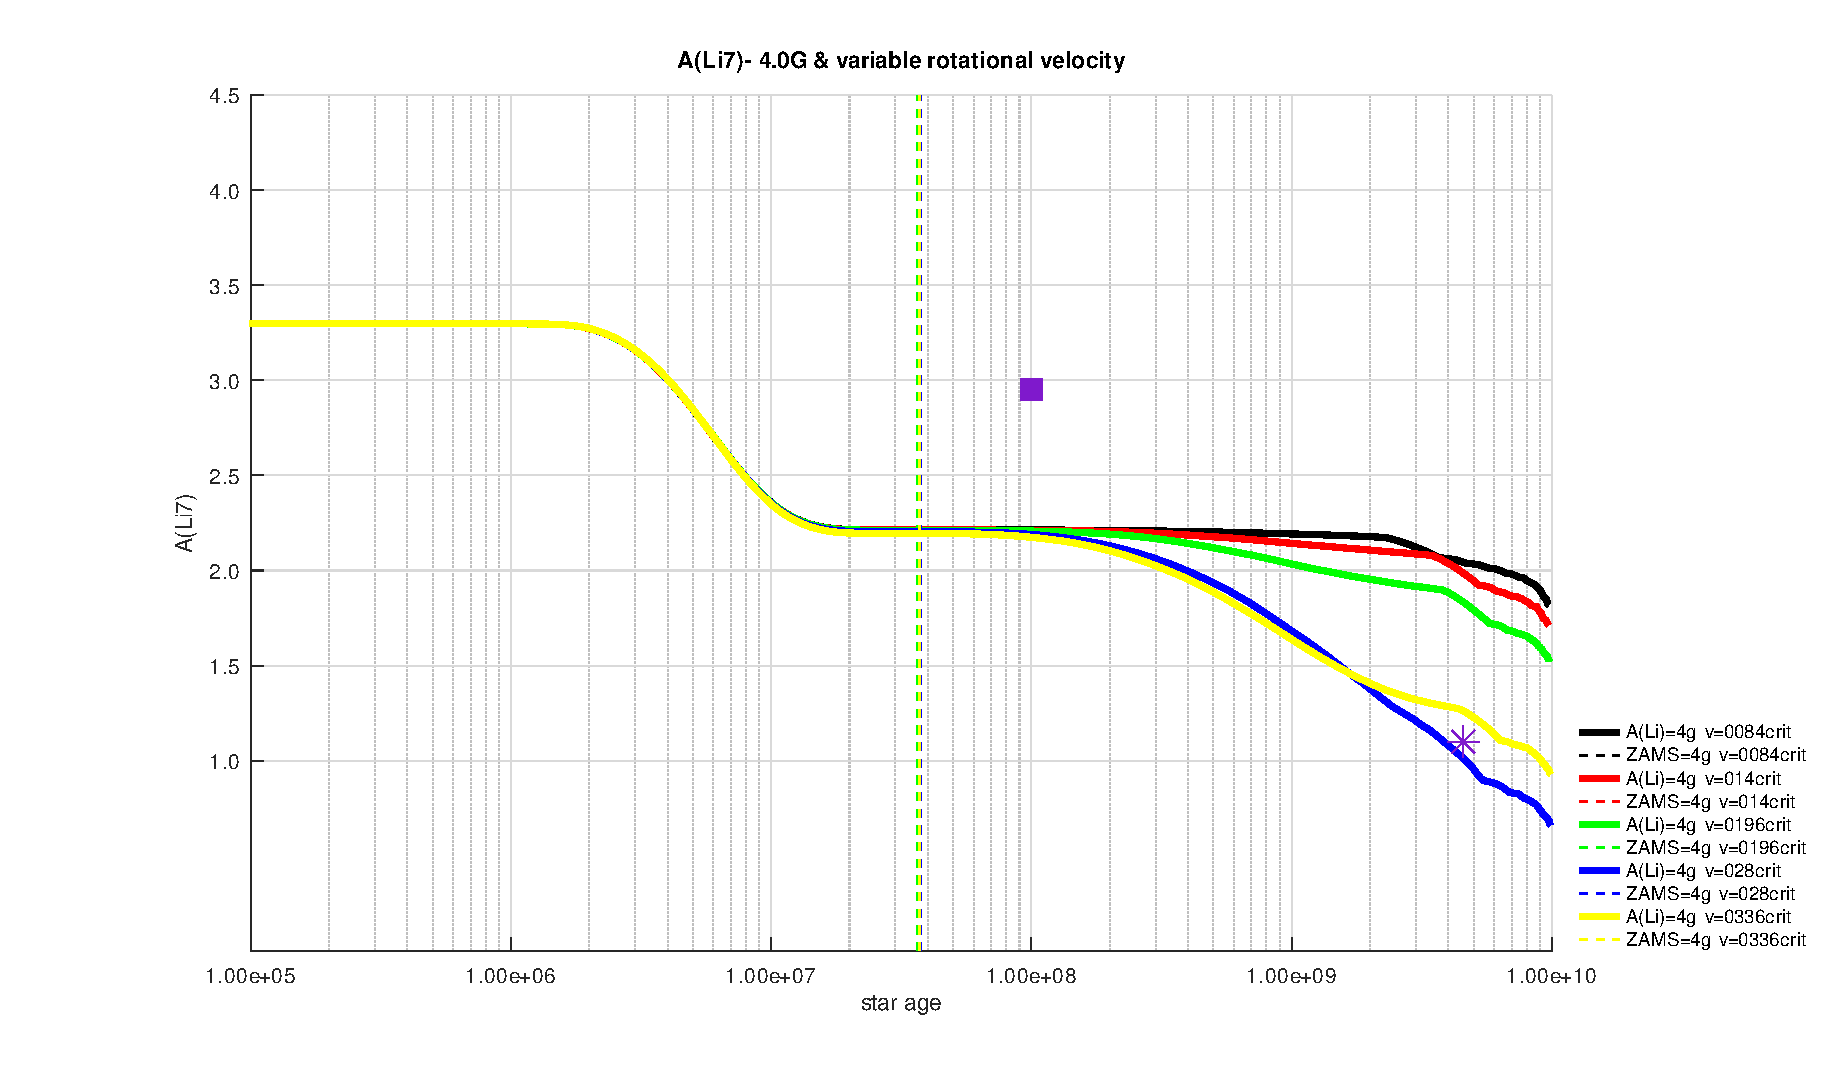
\includegraphics[trim = 40mm 15mm 20mm 15mm, clip,width=\textwidth]{figures/li_var_vel_4_0g.eps}
    \label{fig:subim3}
    \end{subfigure}
    \begin{subfigure}[h]{0.47\textwidth}
    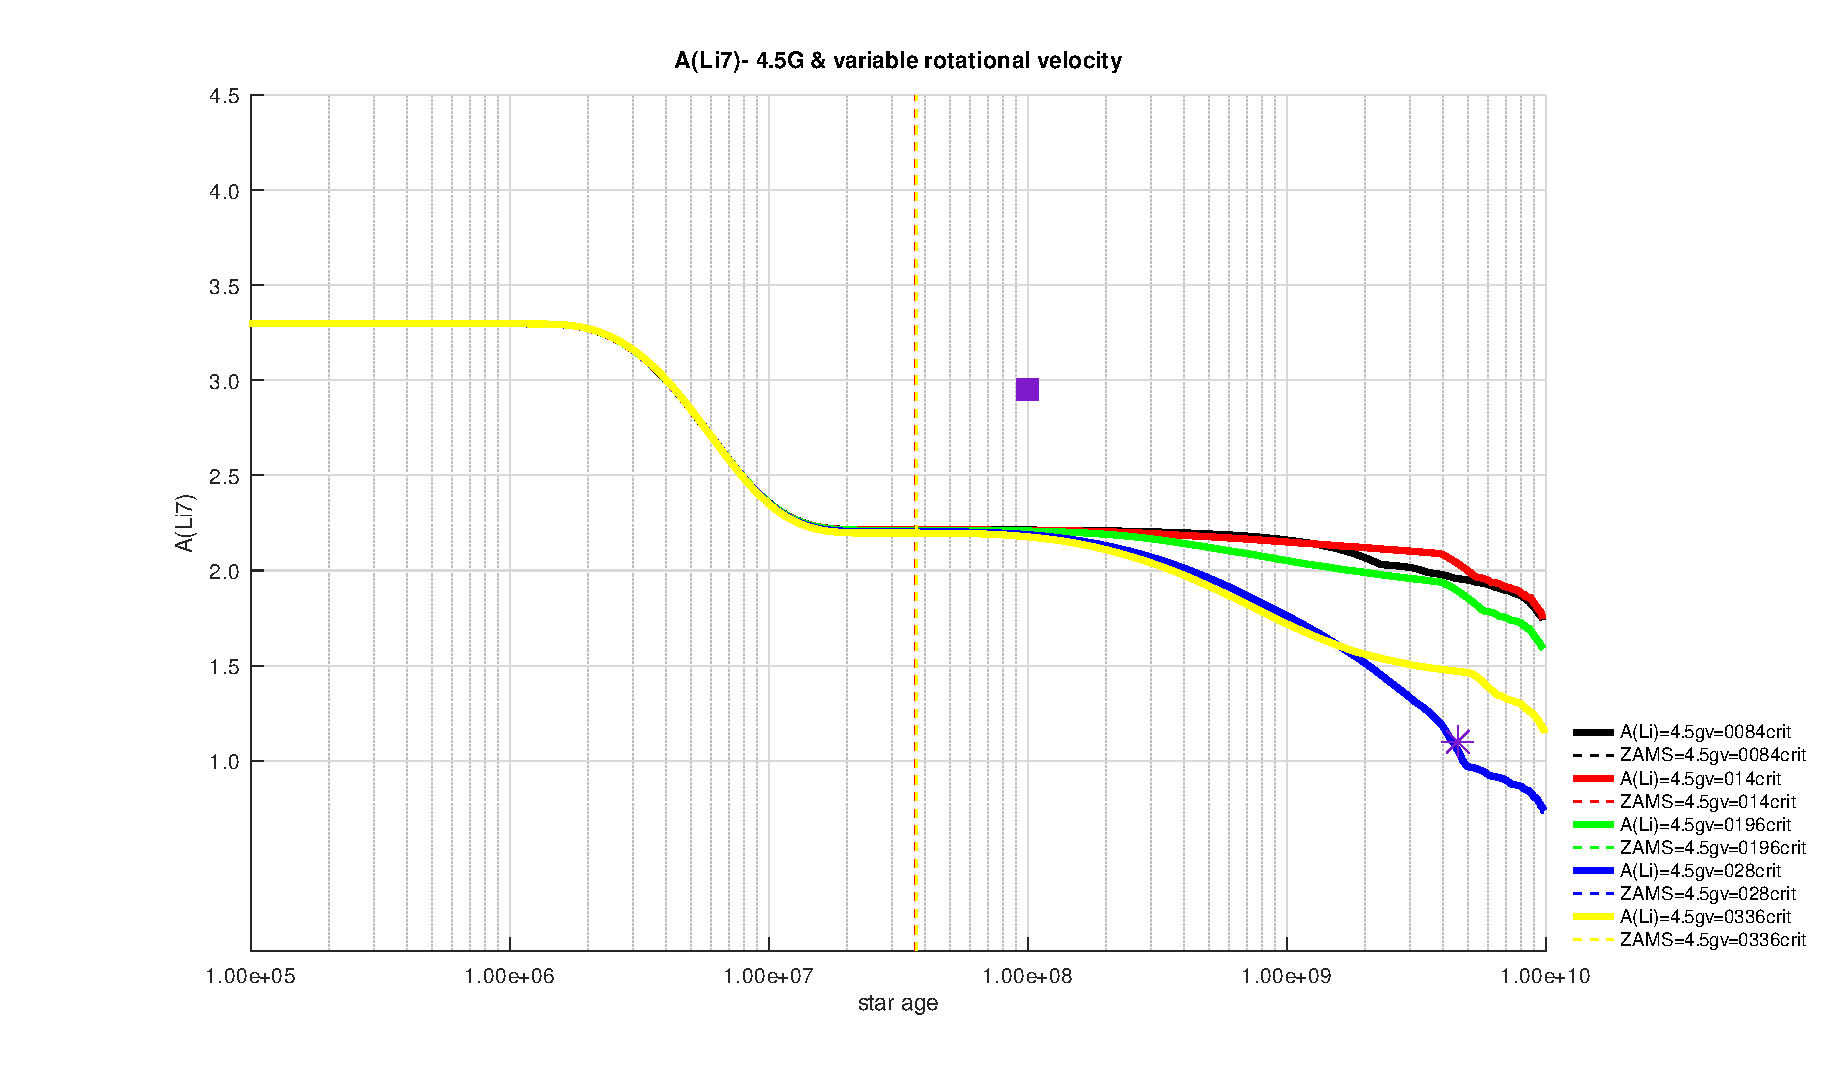
\includegraphics[trim = 40mm 15mm 20mm 15mm, clip,width=\textwidth]{figures/li_var_vel_4_5g.eps}
    \label{fig:subim4}
    \end{subfigure}
    
    \begin{subfigure}[h]{0.47\textwidth}
    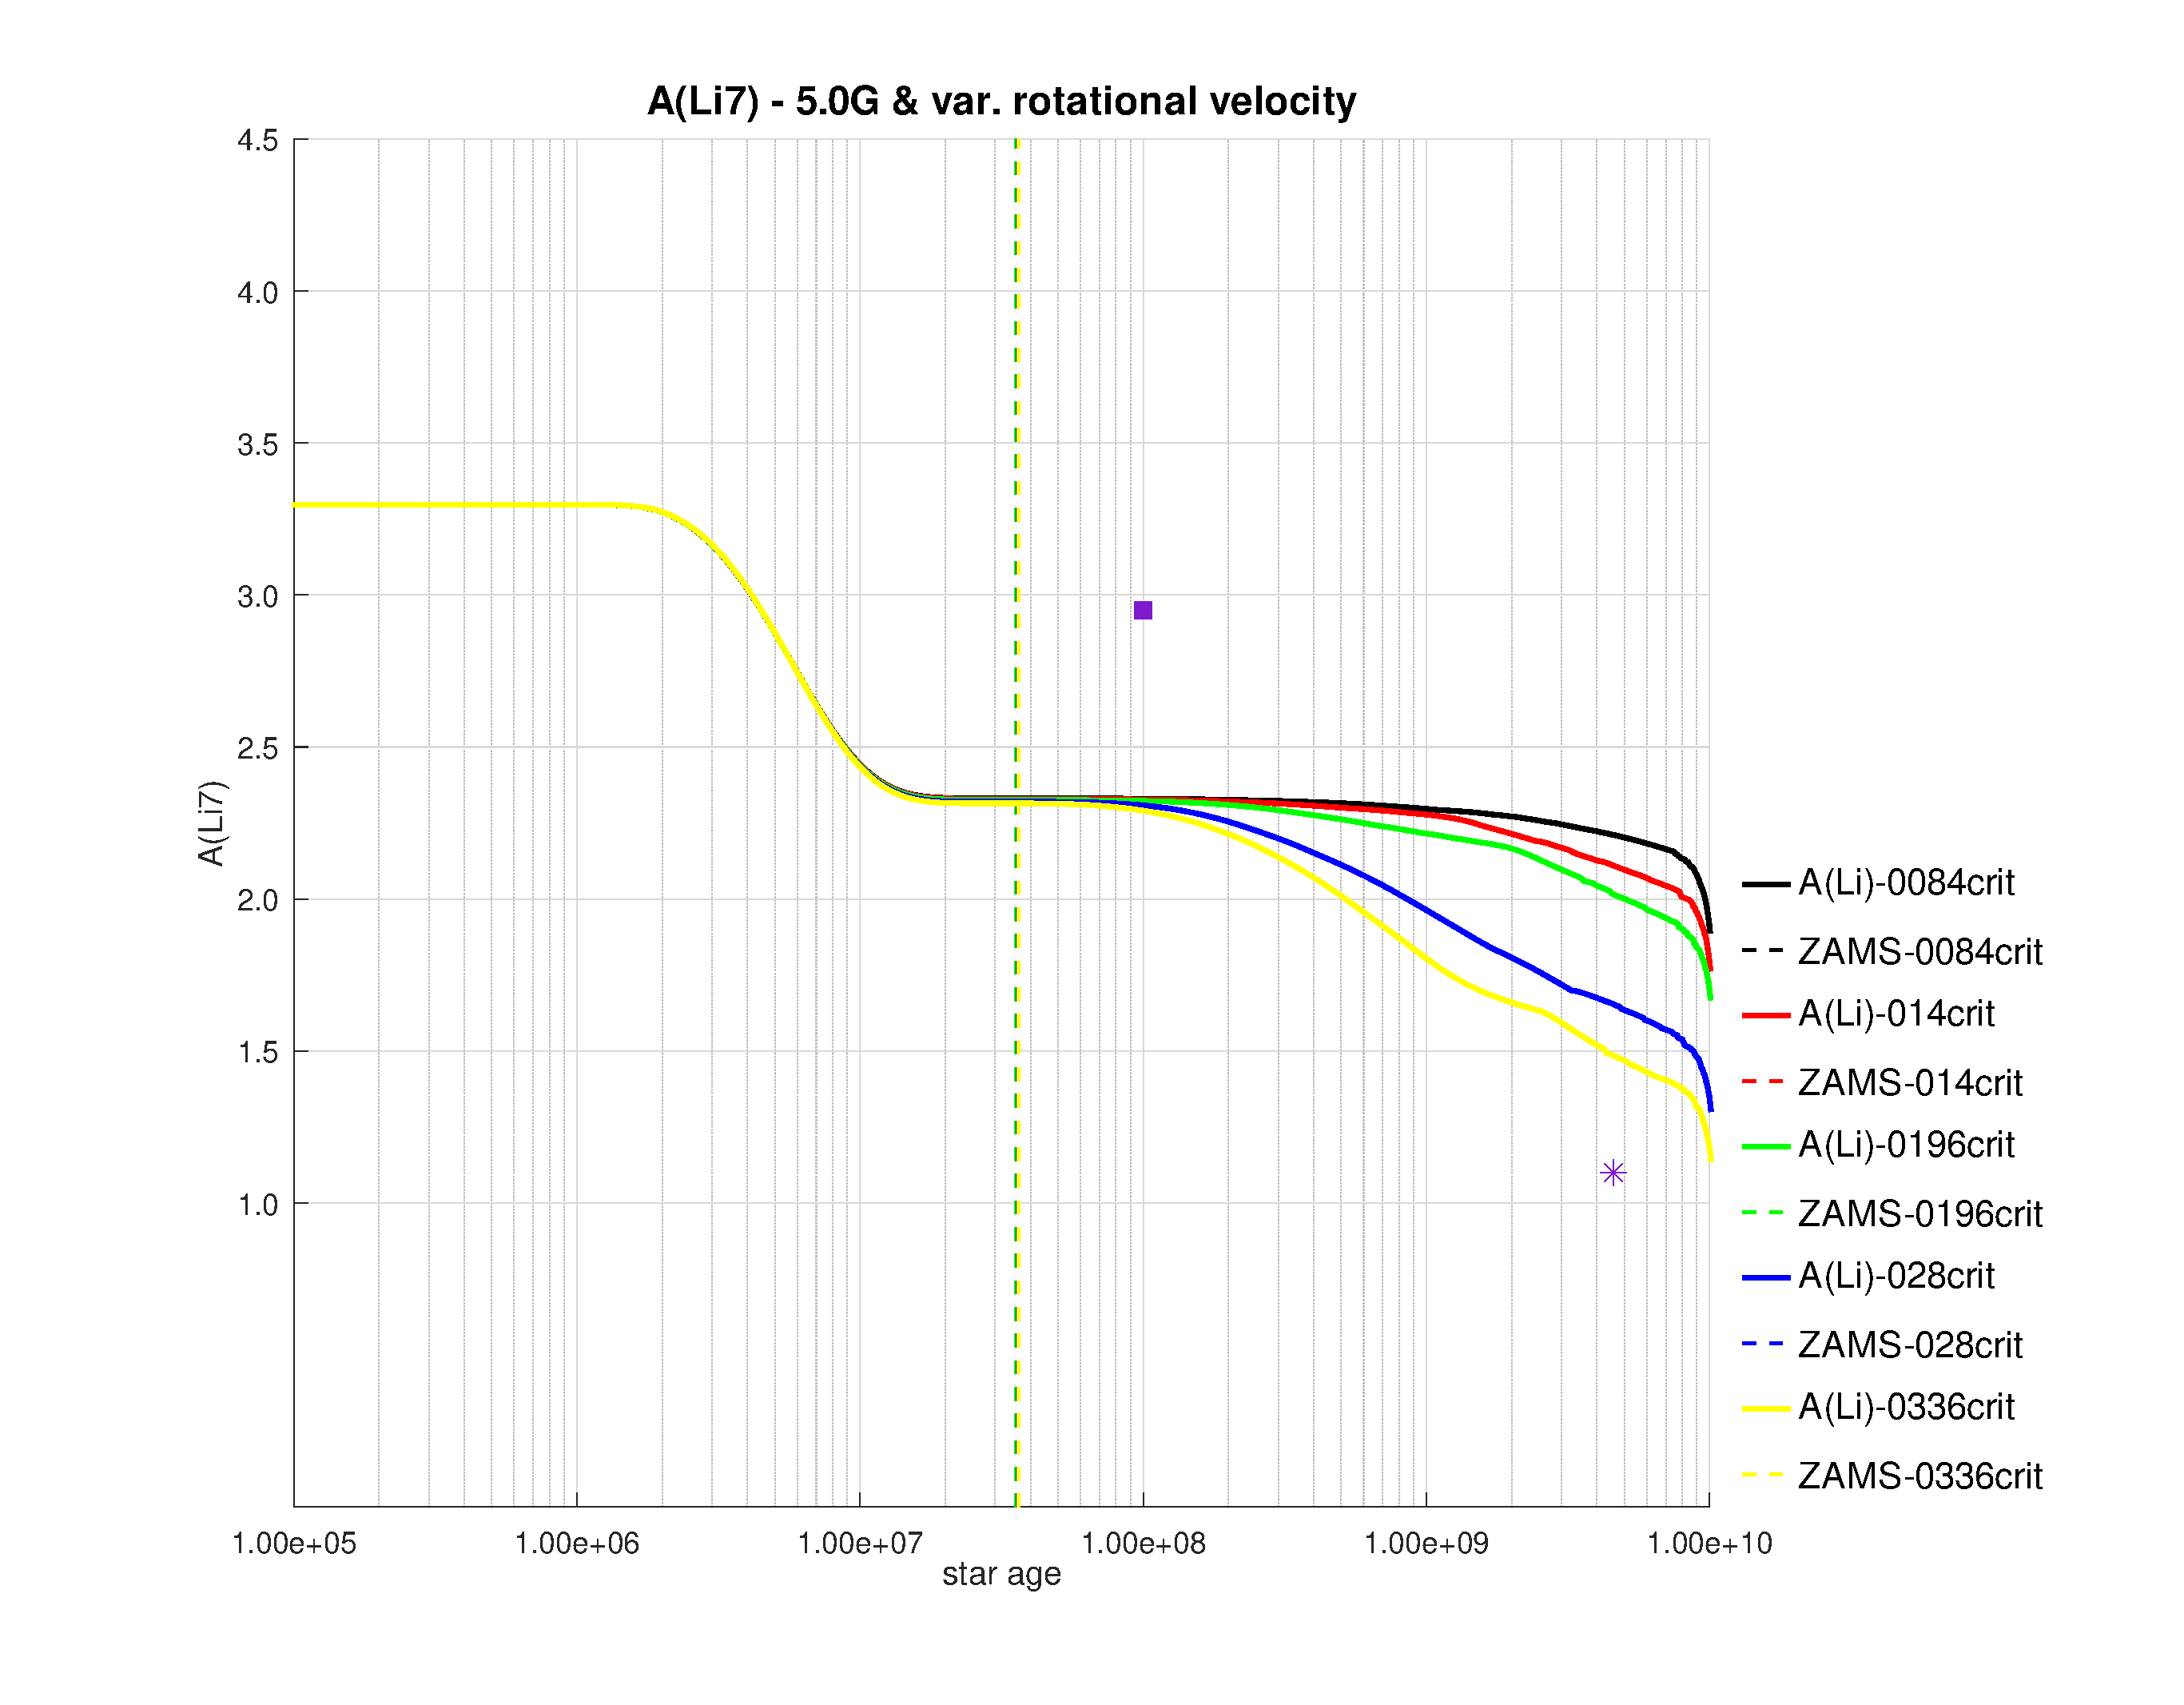
\includegraphics[trim = 40mm 15mm 20mm 15mm, clip,width=\textwidth]{figures/li_var_vel_5_0g.eps}
    \label{fig:subim5}
    \end{subfigure}
    \begin{subfigure}[h]{0.47\textwidth}
    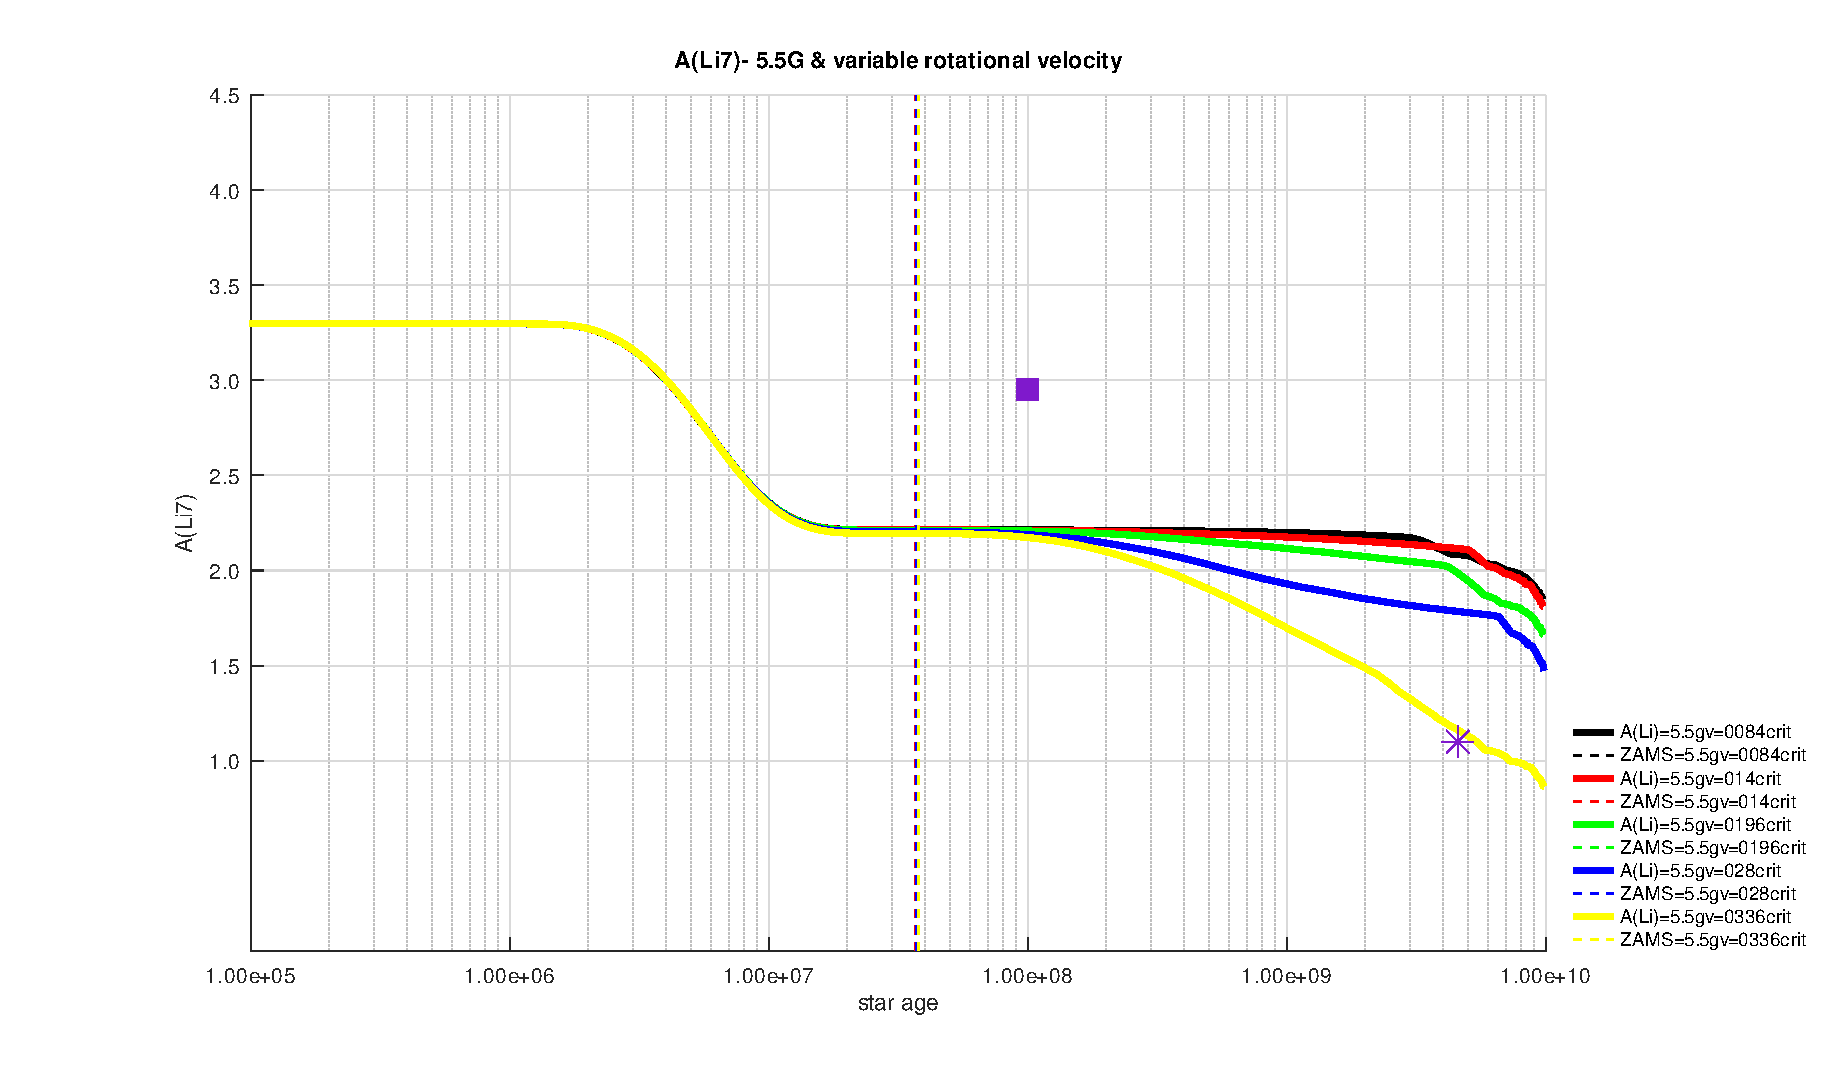
\includegraphics[trim = 40mm 15mm 20mm 15mm, clip,width=\textwidth]{figures/li_var_vel_5_5g.eps}
    \label{fig:subim6}
    \end{subfigure}
\caption{Grid showing the evolution of surface \isotope[7]{Li} abundance relative to \isotope[1]{H}, as a function of time for several 1 $M_{\sun}$ models. Each figure shows a set of models in which the magnetic field with intensity has been fixed and $\Omega / \Omega_{crit}$ varies between 0.0084 and 0.0336, respectively. The purple star and square are surface Li abundance for the present-day Sun \citep{Asplund2009} and the Pleiades cluster \citep{Sestito2005} respectively. The dashed lines make reference to the ZAMS.}
\label{fig:grid_li_var_vel}
\end{figure*}
\par


\begin{figure*}
    \centering
    \begin{subfigure}[h]{0.47\textwidth}
    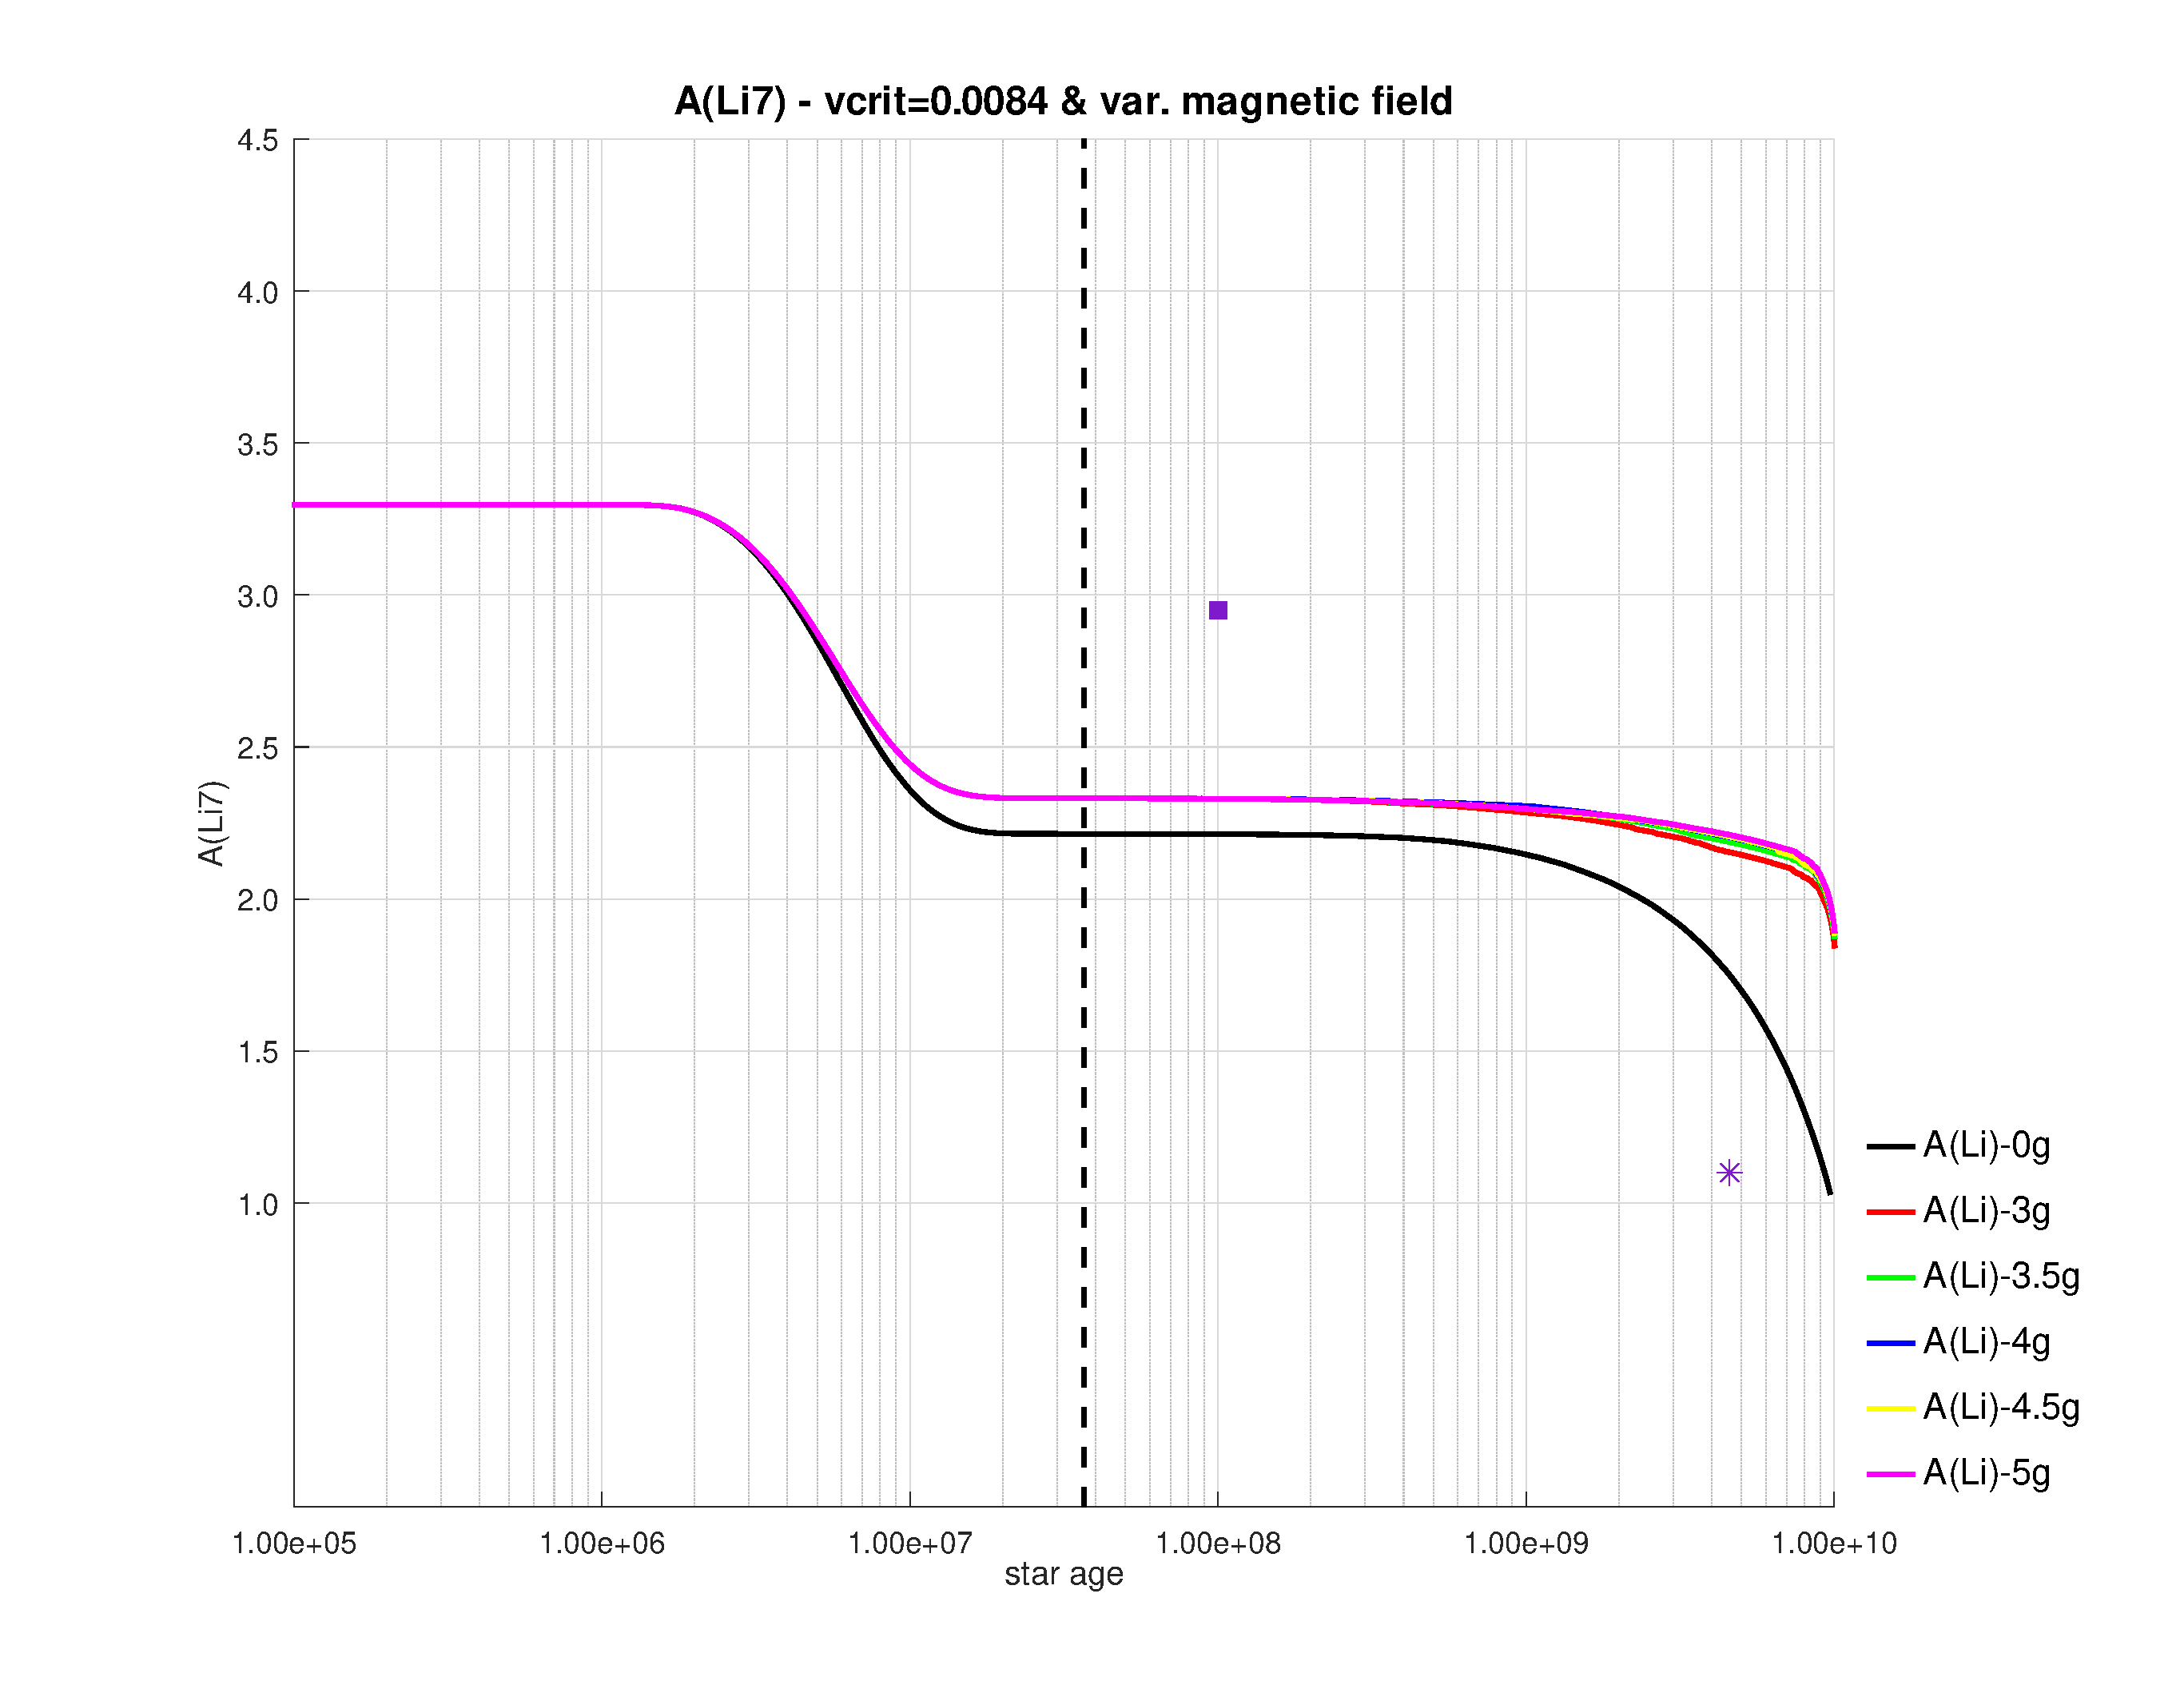
\includegraphics[trim = 40mm 15mm 15mm 15mm, clip,width=\textwidth]{figures/li_vc_0084_var_g.eps}
    \label{fig:subim21}
    \end{subfigure}
    \begin{subfigure}[h]{0.47\textwidth}
    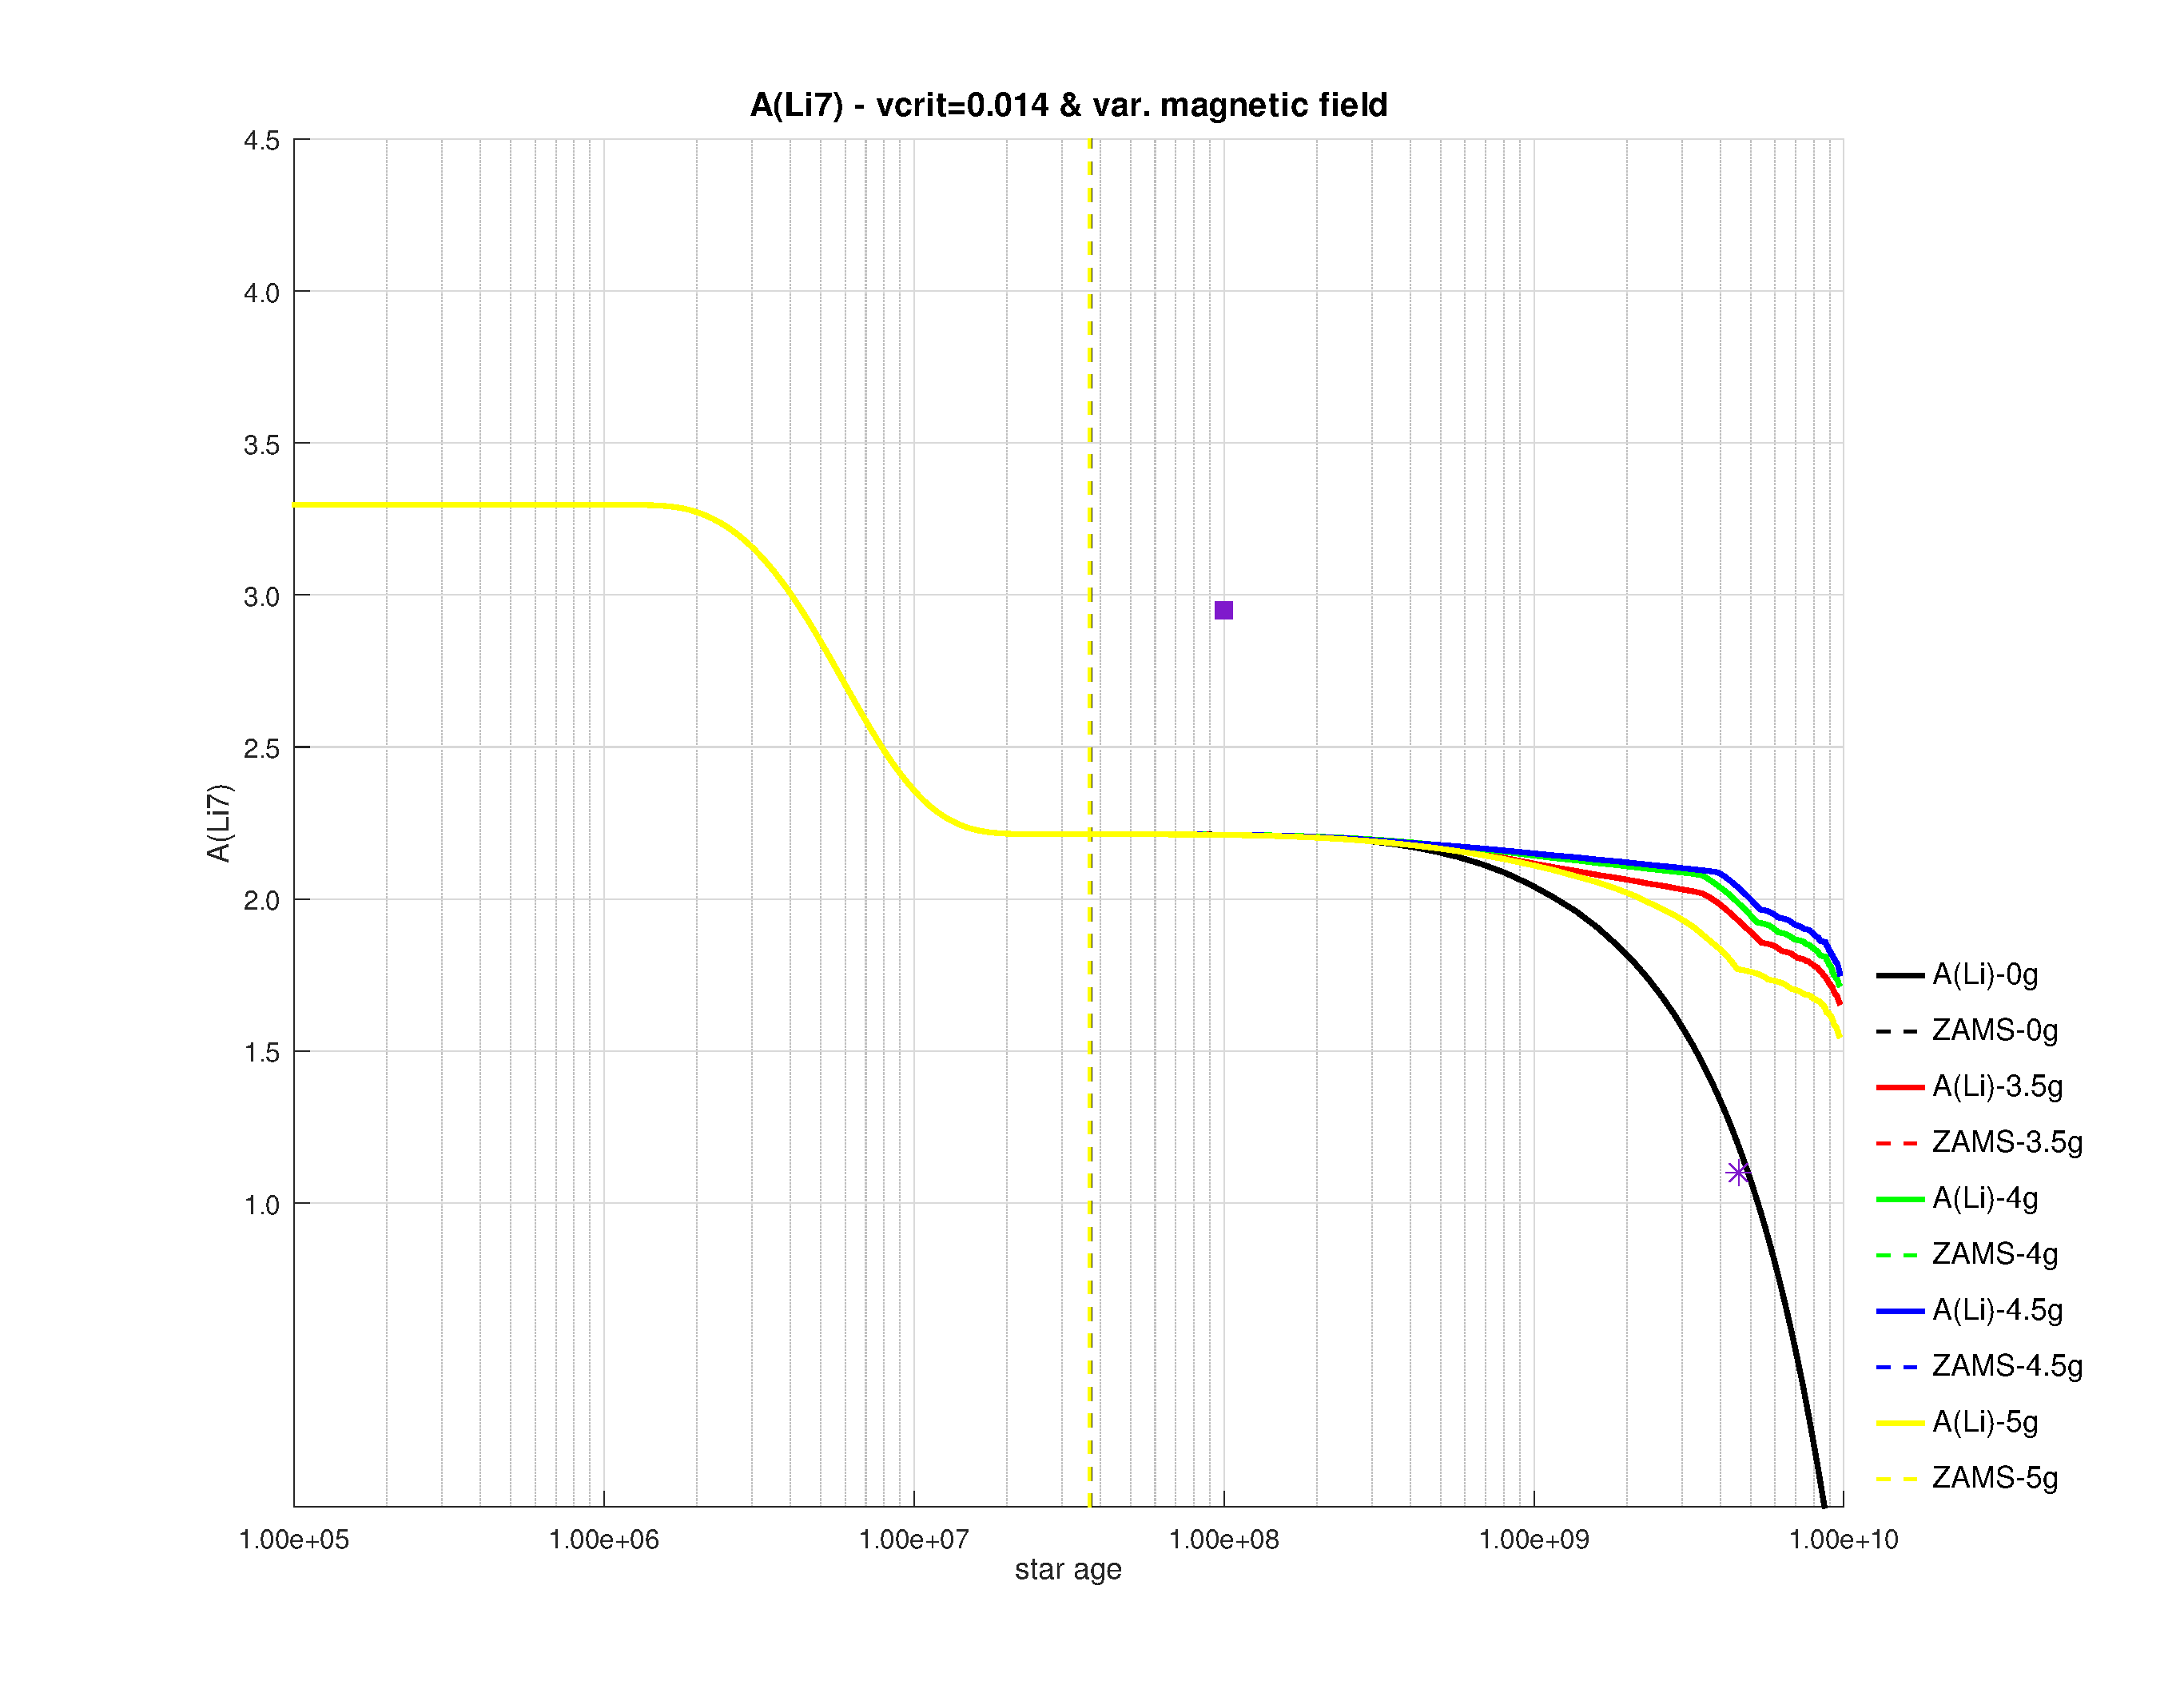
\includegraphics[trim = 40mm 15mm 15mm 15mm, clip,width=\textwidth]{figures/li_vc_014_var_g.eps}
    \label{fig:subim22}
    \end{subfigure}
    \begin{subfigure}[h]{0.47\textwidth}
    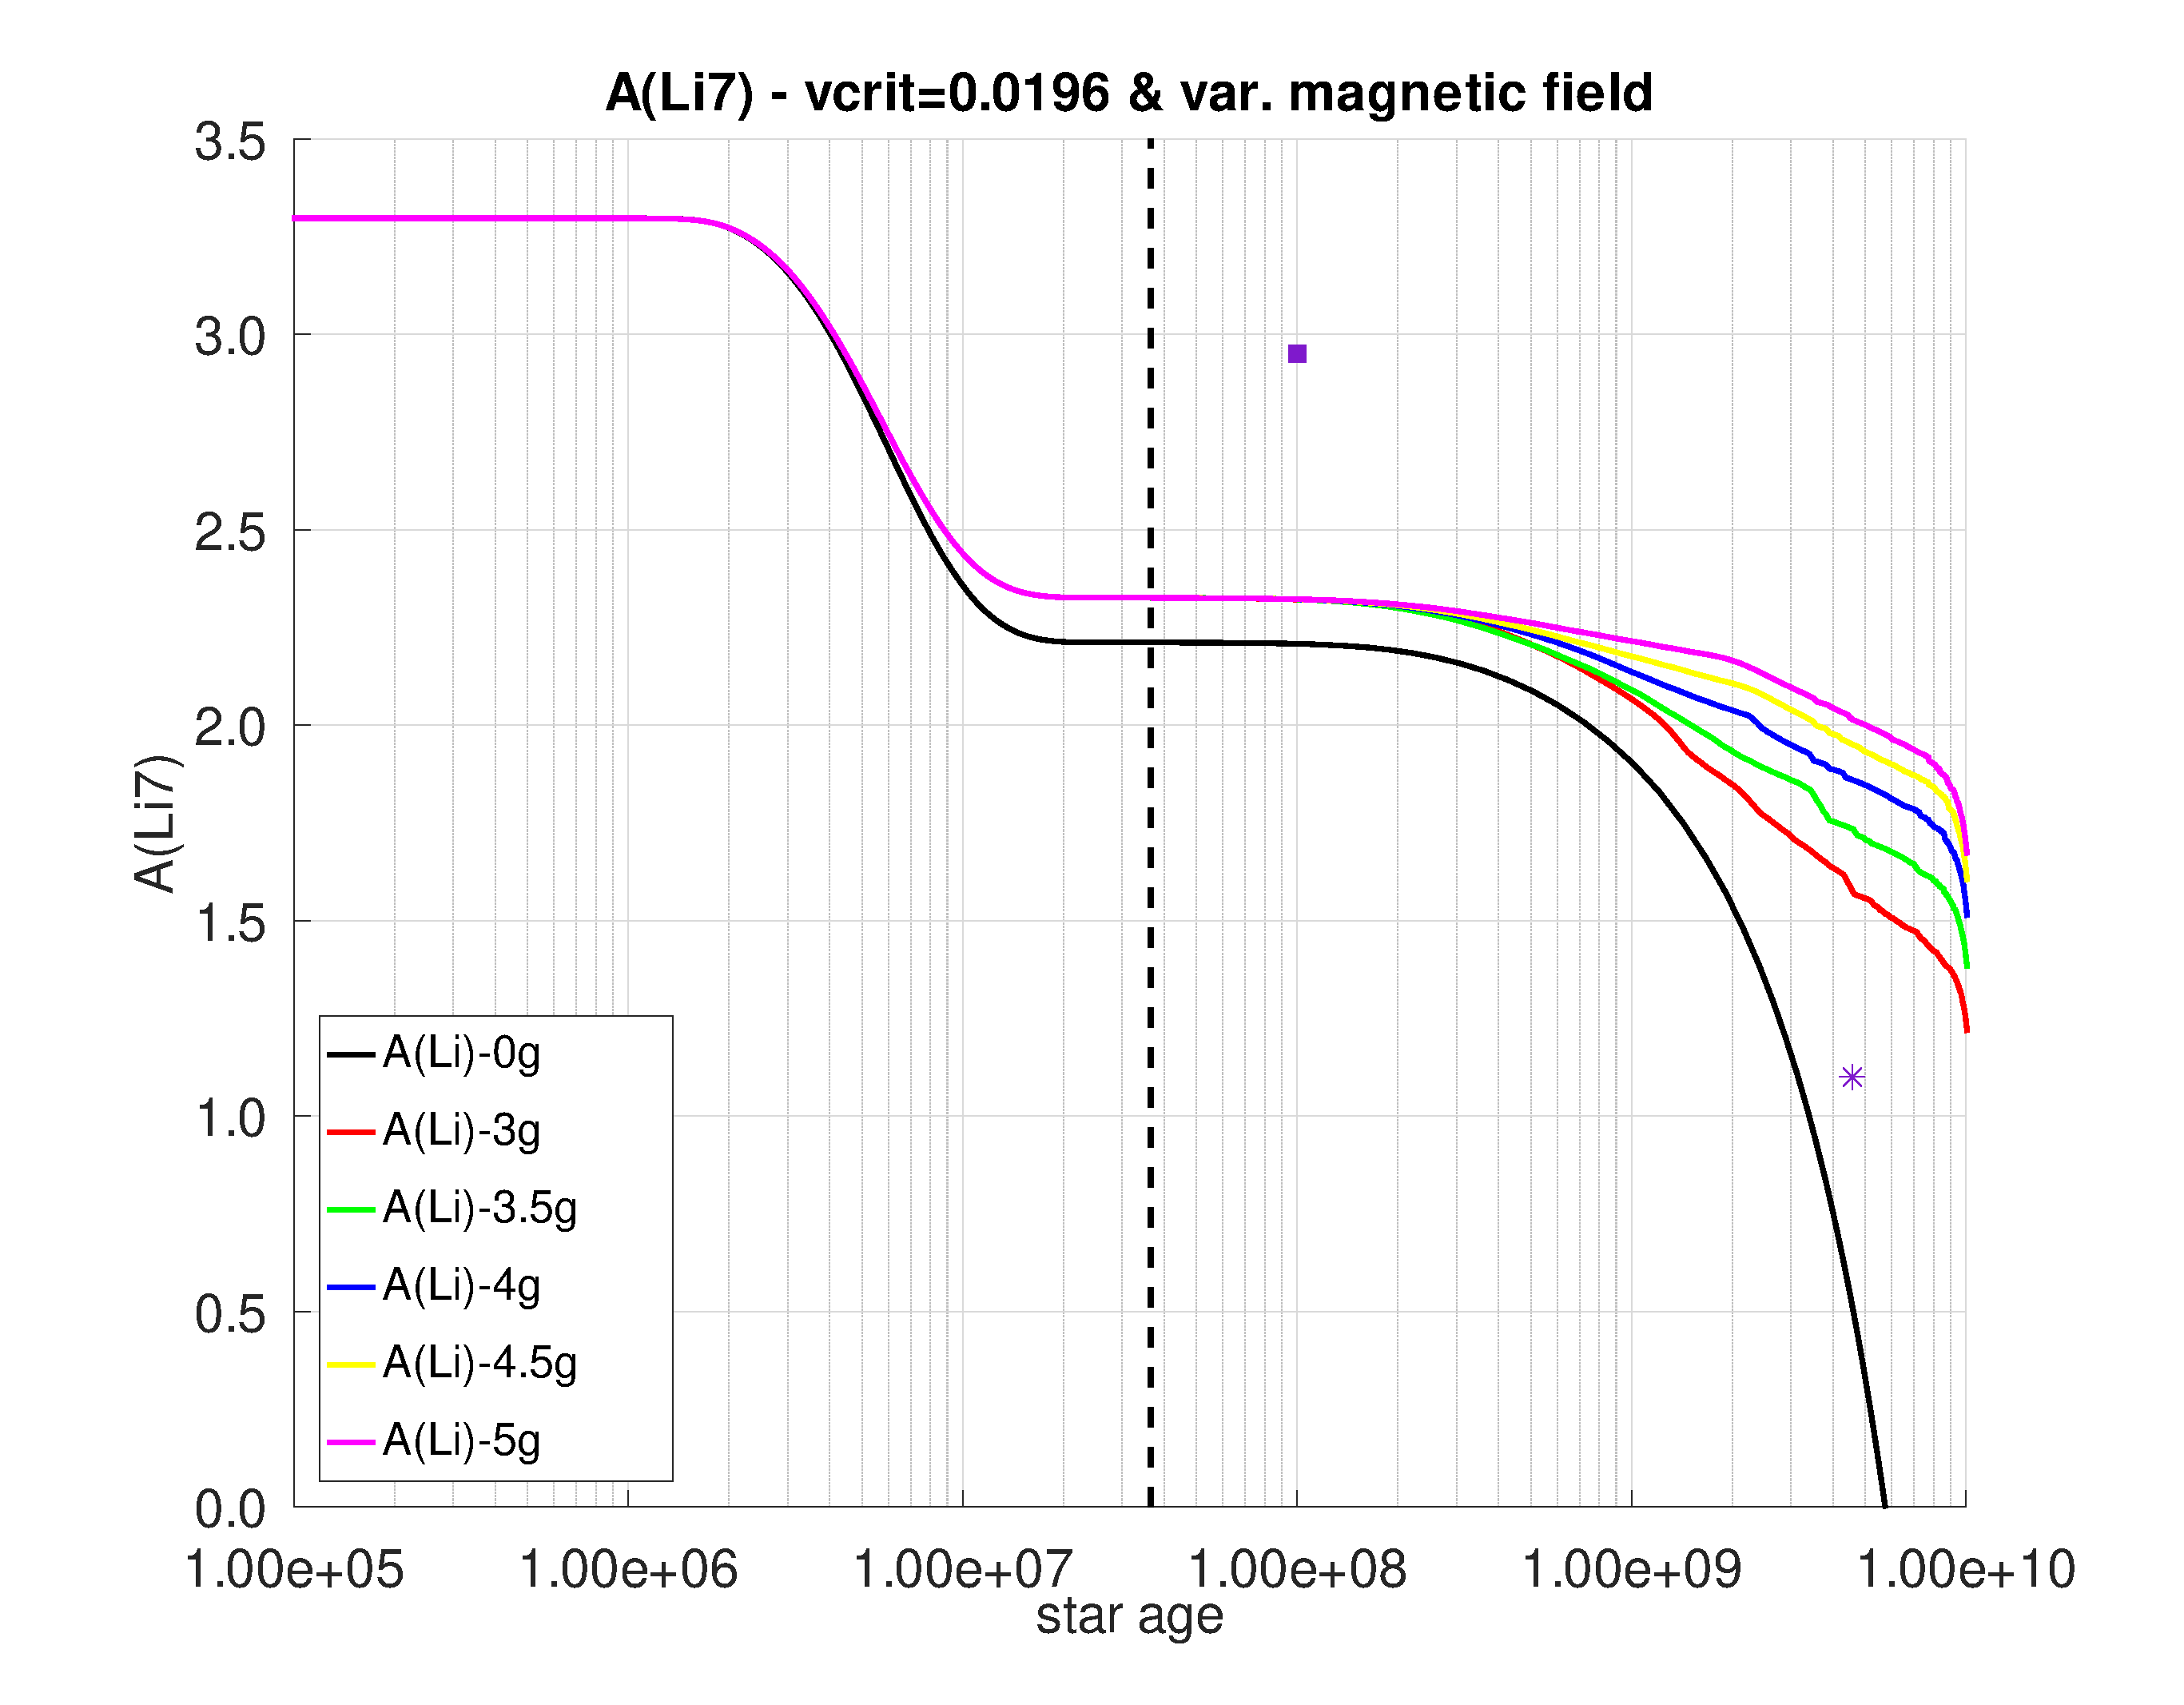
\includegraphics[trim = 40mm 15mm 15mm 15mm, clip,width=\textwidth]{figures/li_vc_0196_var_g.eps}
    \label{fig:subim23}
    \end{subfigure}
    \begin{subfigure}[h]{0.47\textwidth}
    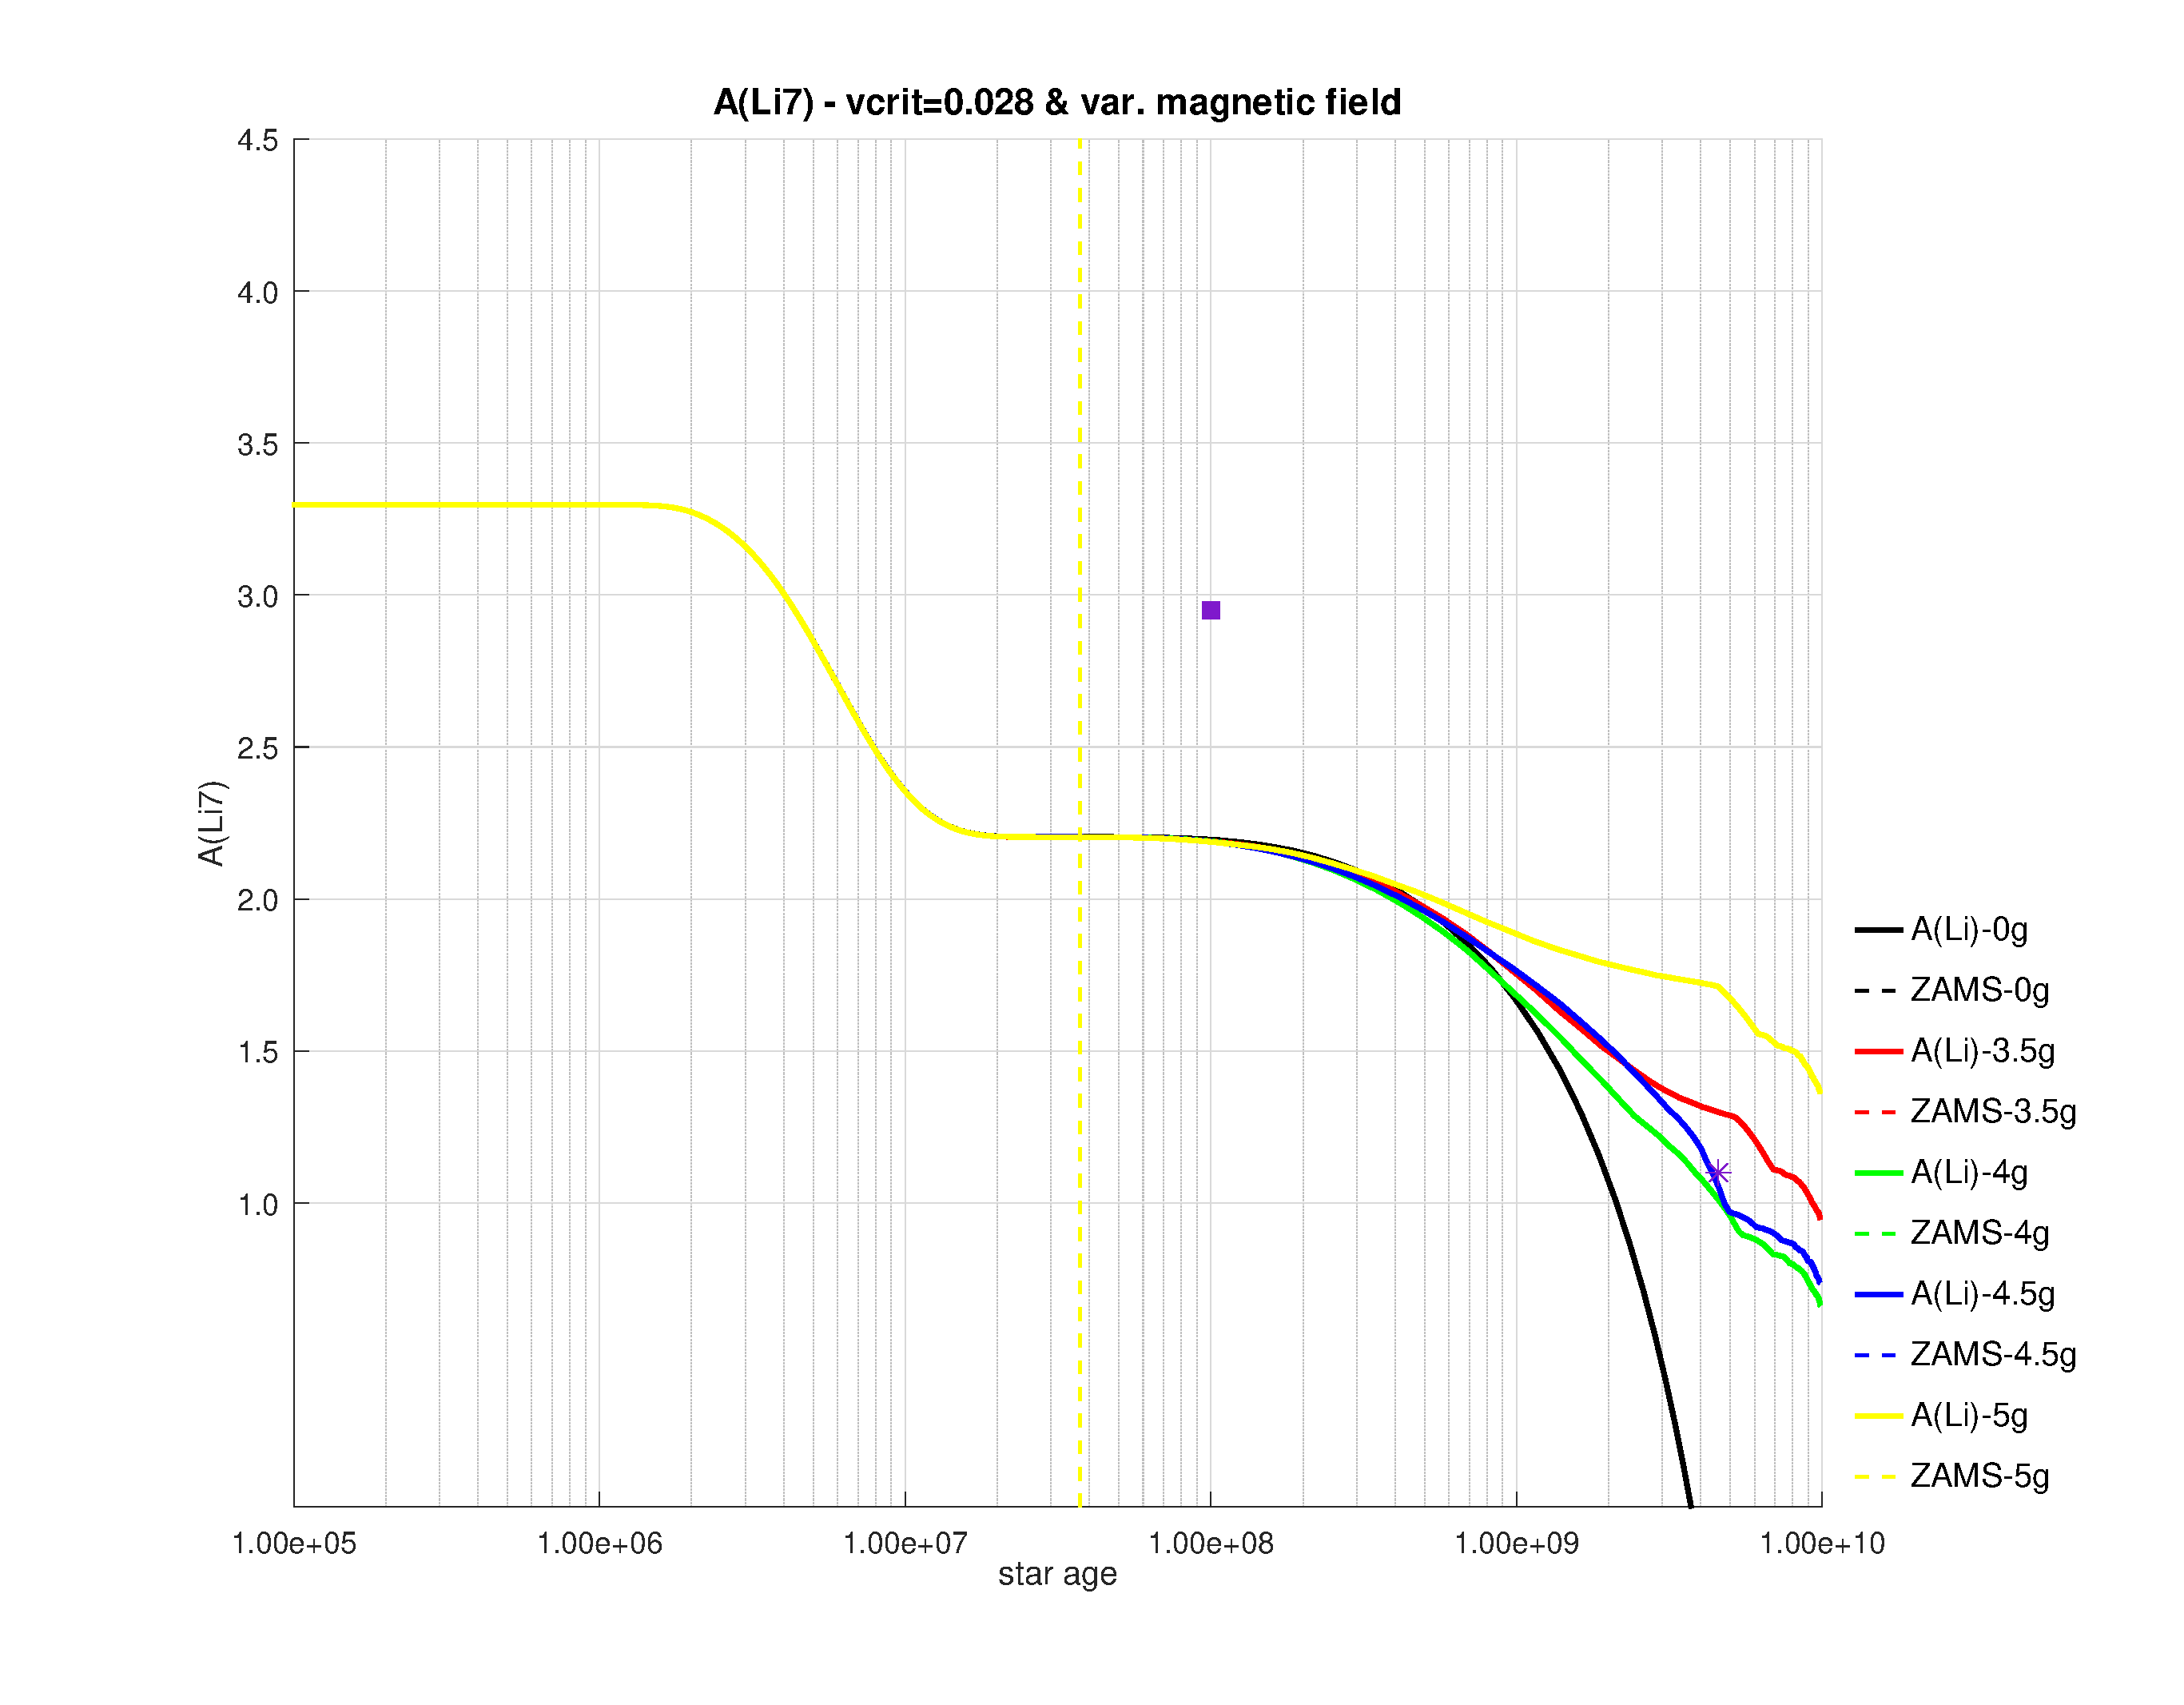
\includegraphics[trim = 40mm 15mm 15mm 15mm, clip,width=\textwidth]{figures/li_vc_028_var_g.eps}
    \label{fig:subim24}
    \end{subfigure}
    \begin{subfigure}[h]{0.47\textwidth}
    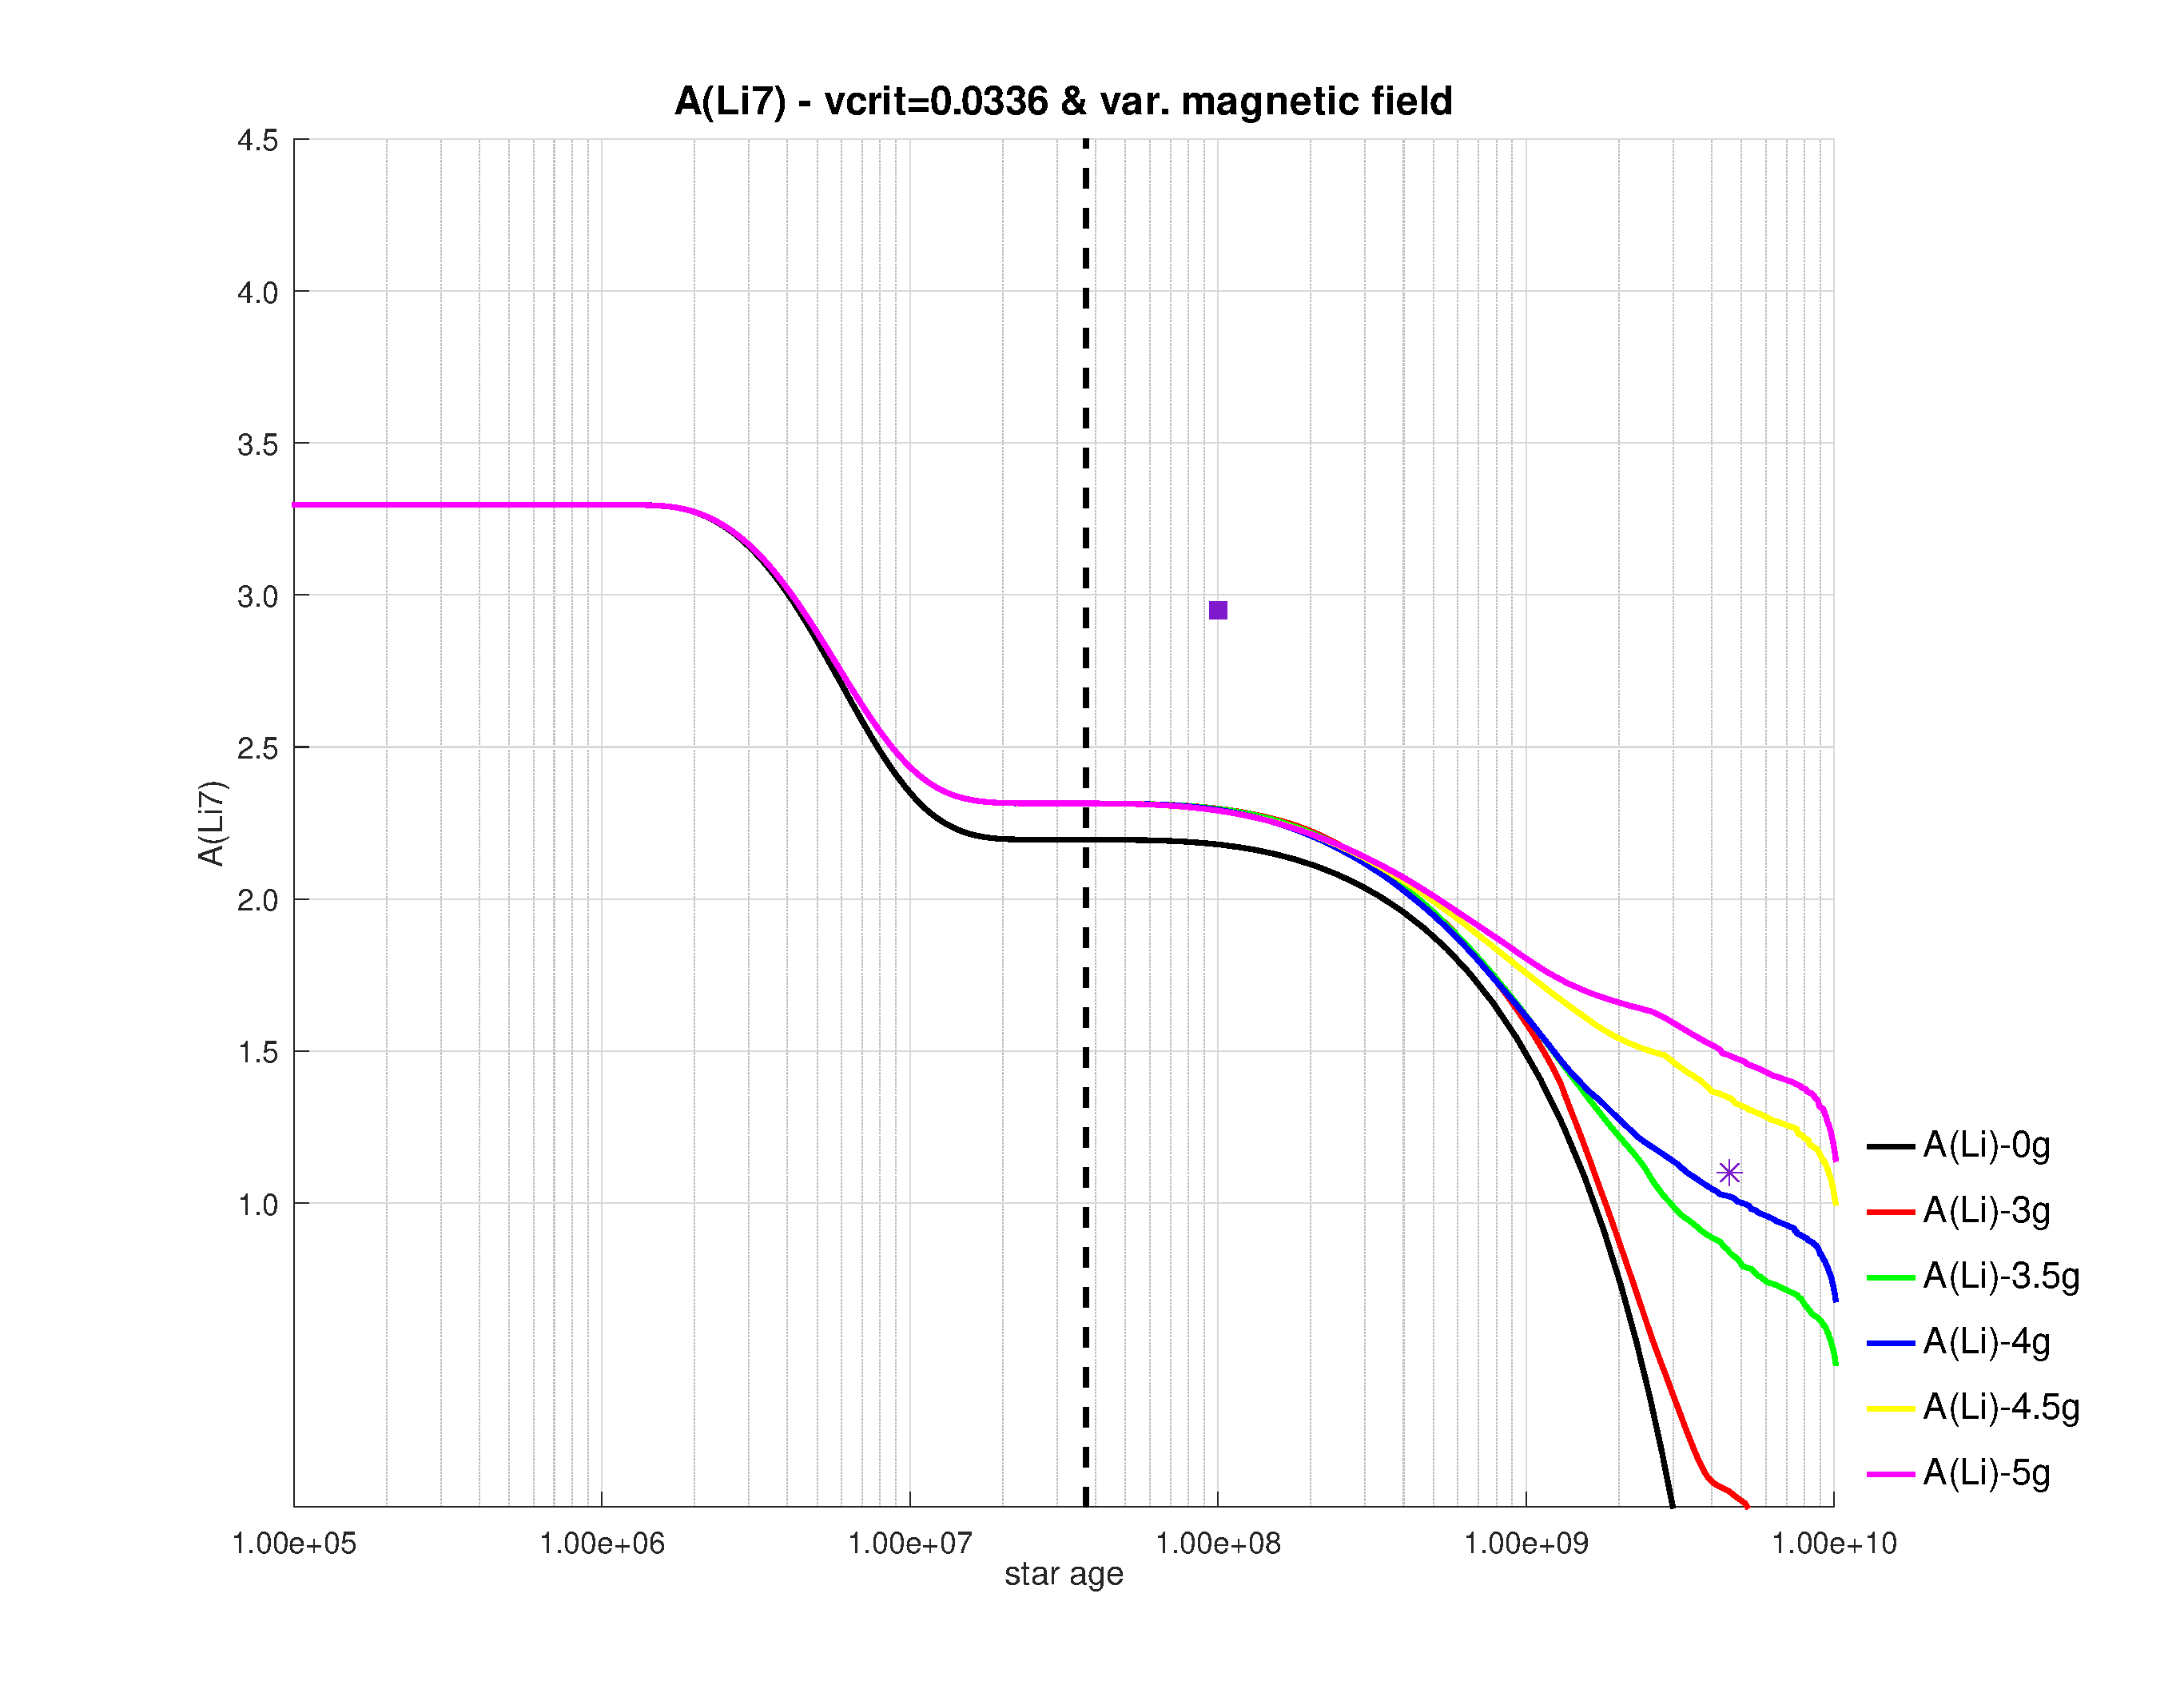
\includegraphics[trim = 40mm 15mm 15mm 15mm, clip,width=\textwidth]{figures/li_vc_0336_var_g.eps}
    \label{fig:subim25}
    \end{subfigure}
    \begin{subfigure}[h]{0.47\textwidth}
    \includegraphics[width=\textwidth]{figures/blank.eps}
    \label{fig:subim26}
    \end{subfigure}
\caption{Grid showing the evolution of surface \isotope[7]{Li} abundance relative to \isotope[1]{H}, as a function of time for several 1 $M_{\sun}$ models. Each figure shows a set of models in which $\Omega / \Omega_{crit}$ has been fixed and the magnetic field with intensity varies between $3.5\,G$ and $5.5\,G$, respectively. The purple star and square are surface Li abundance for the present-day Sun \citep{Asplund2009} and the Pleiades cluster \citep{Sestito2005} respectively. The dashed lines make reference to the ZAMS.}
\label{fig:grid_li_var_g}
\end{figure*}

\begin{figure*}
    \centering
    \begin{subfigure}[h]{0.47\textwidth}
    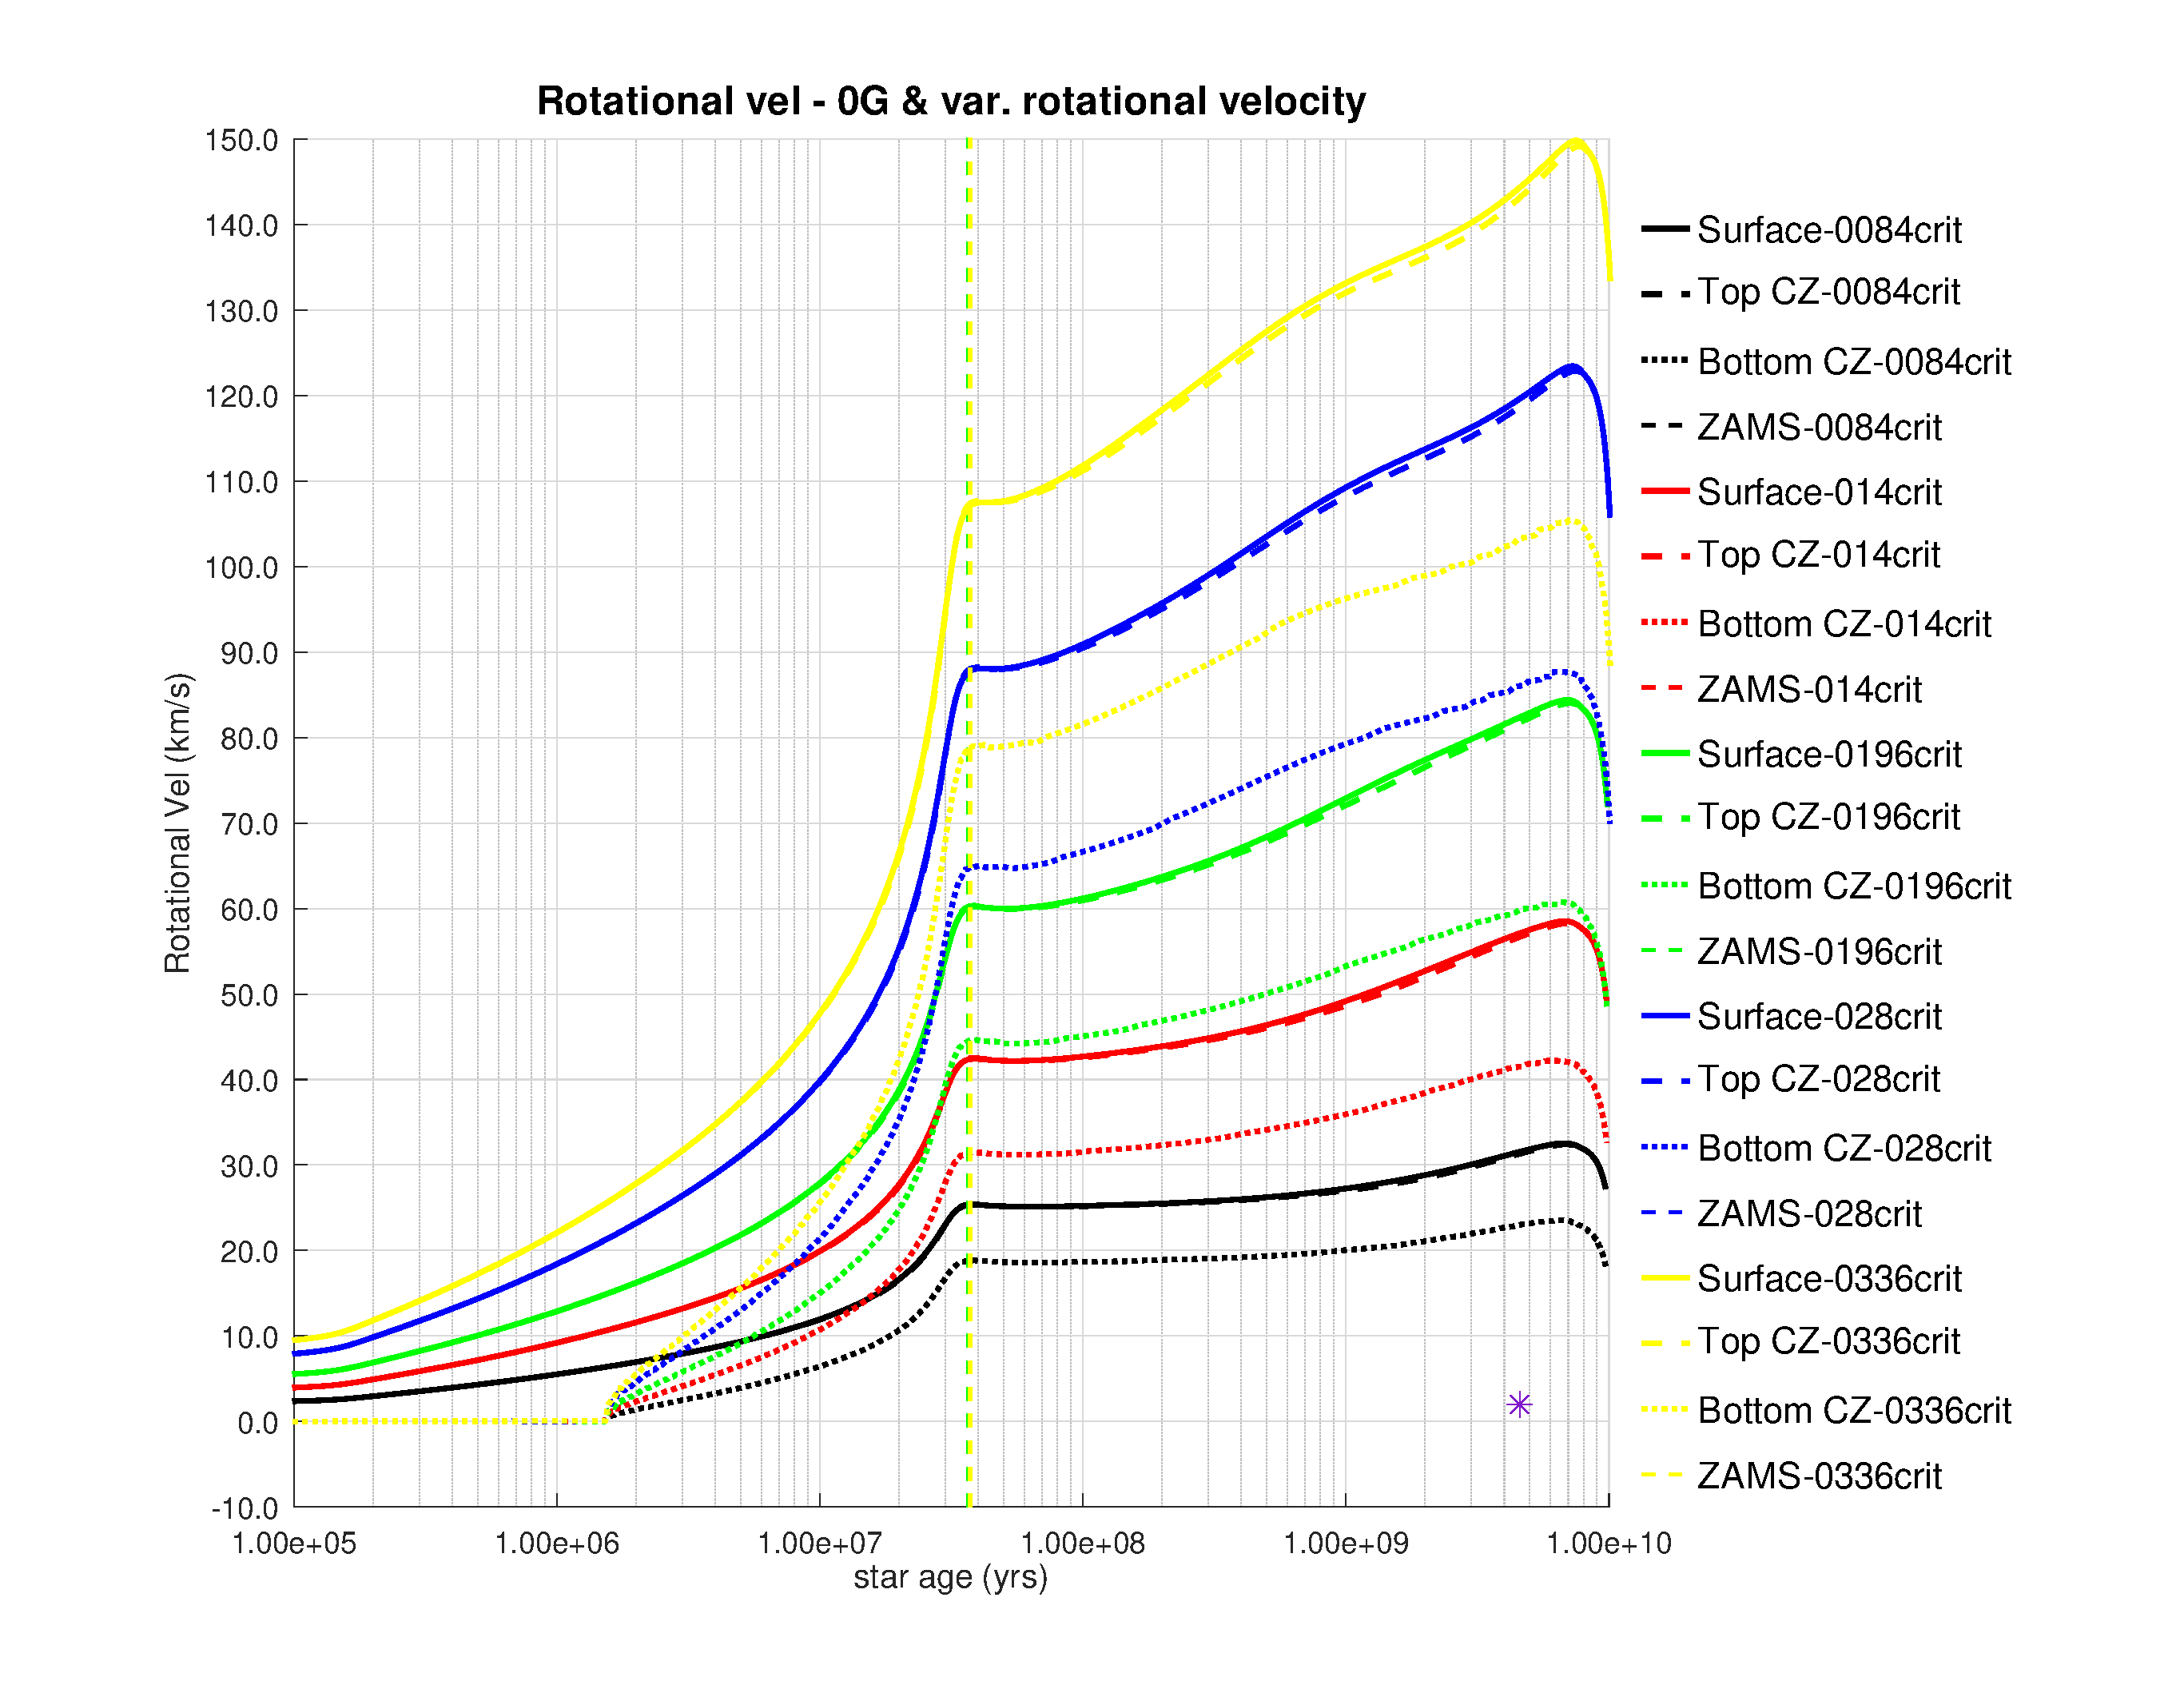
\includegraphics[trim = 30mm 15mm 20mm 15mm, clip,width=\textwidth]{figures/rot_vel_var_vel_0_0g.eps}
    \label{fig:subim41}
    \end{subfigure}
    \begin{subfigure}[h]{0.47\textwidth}
    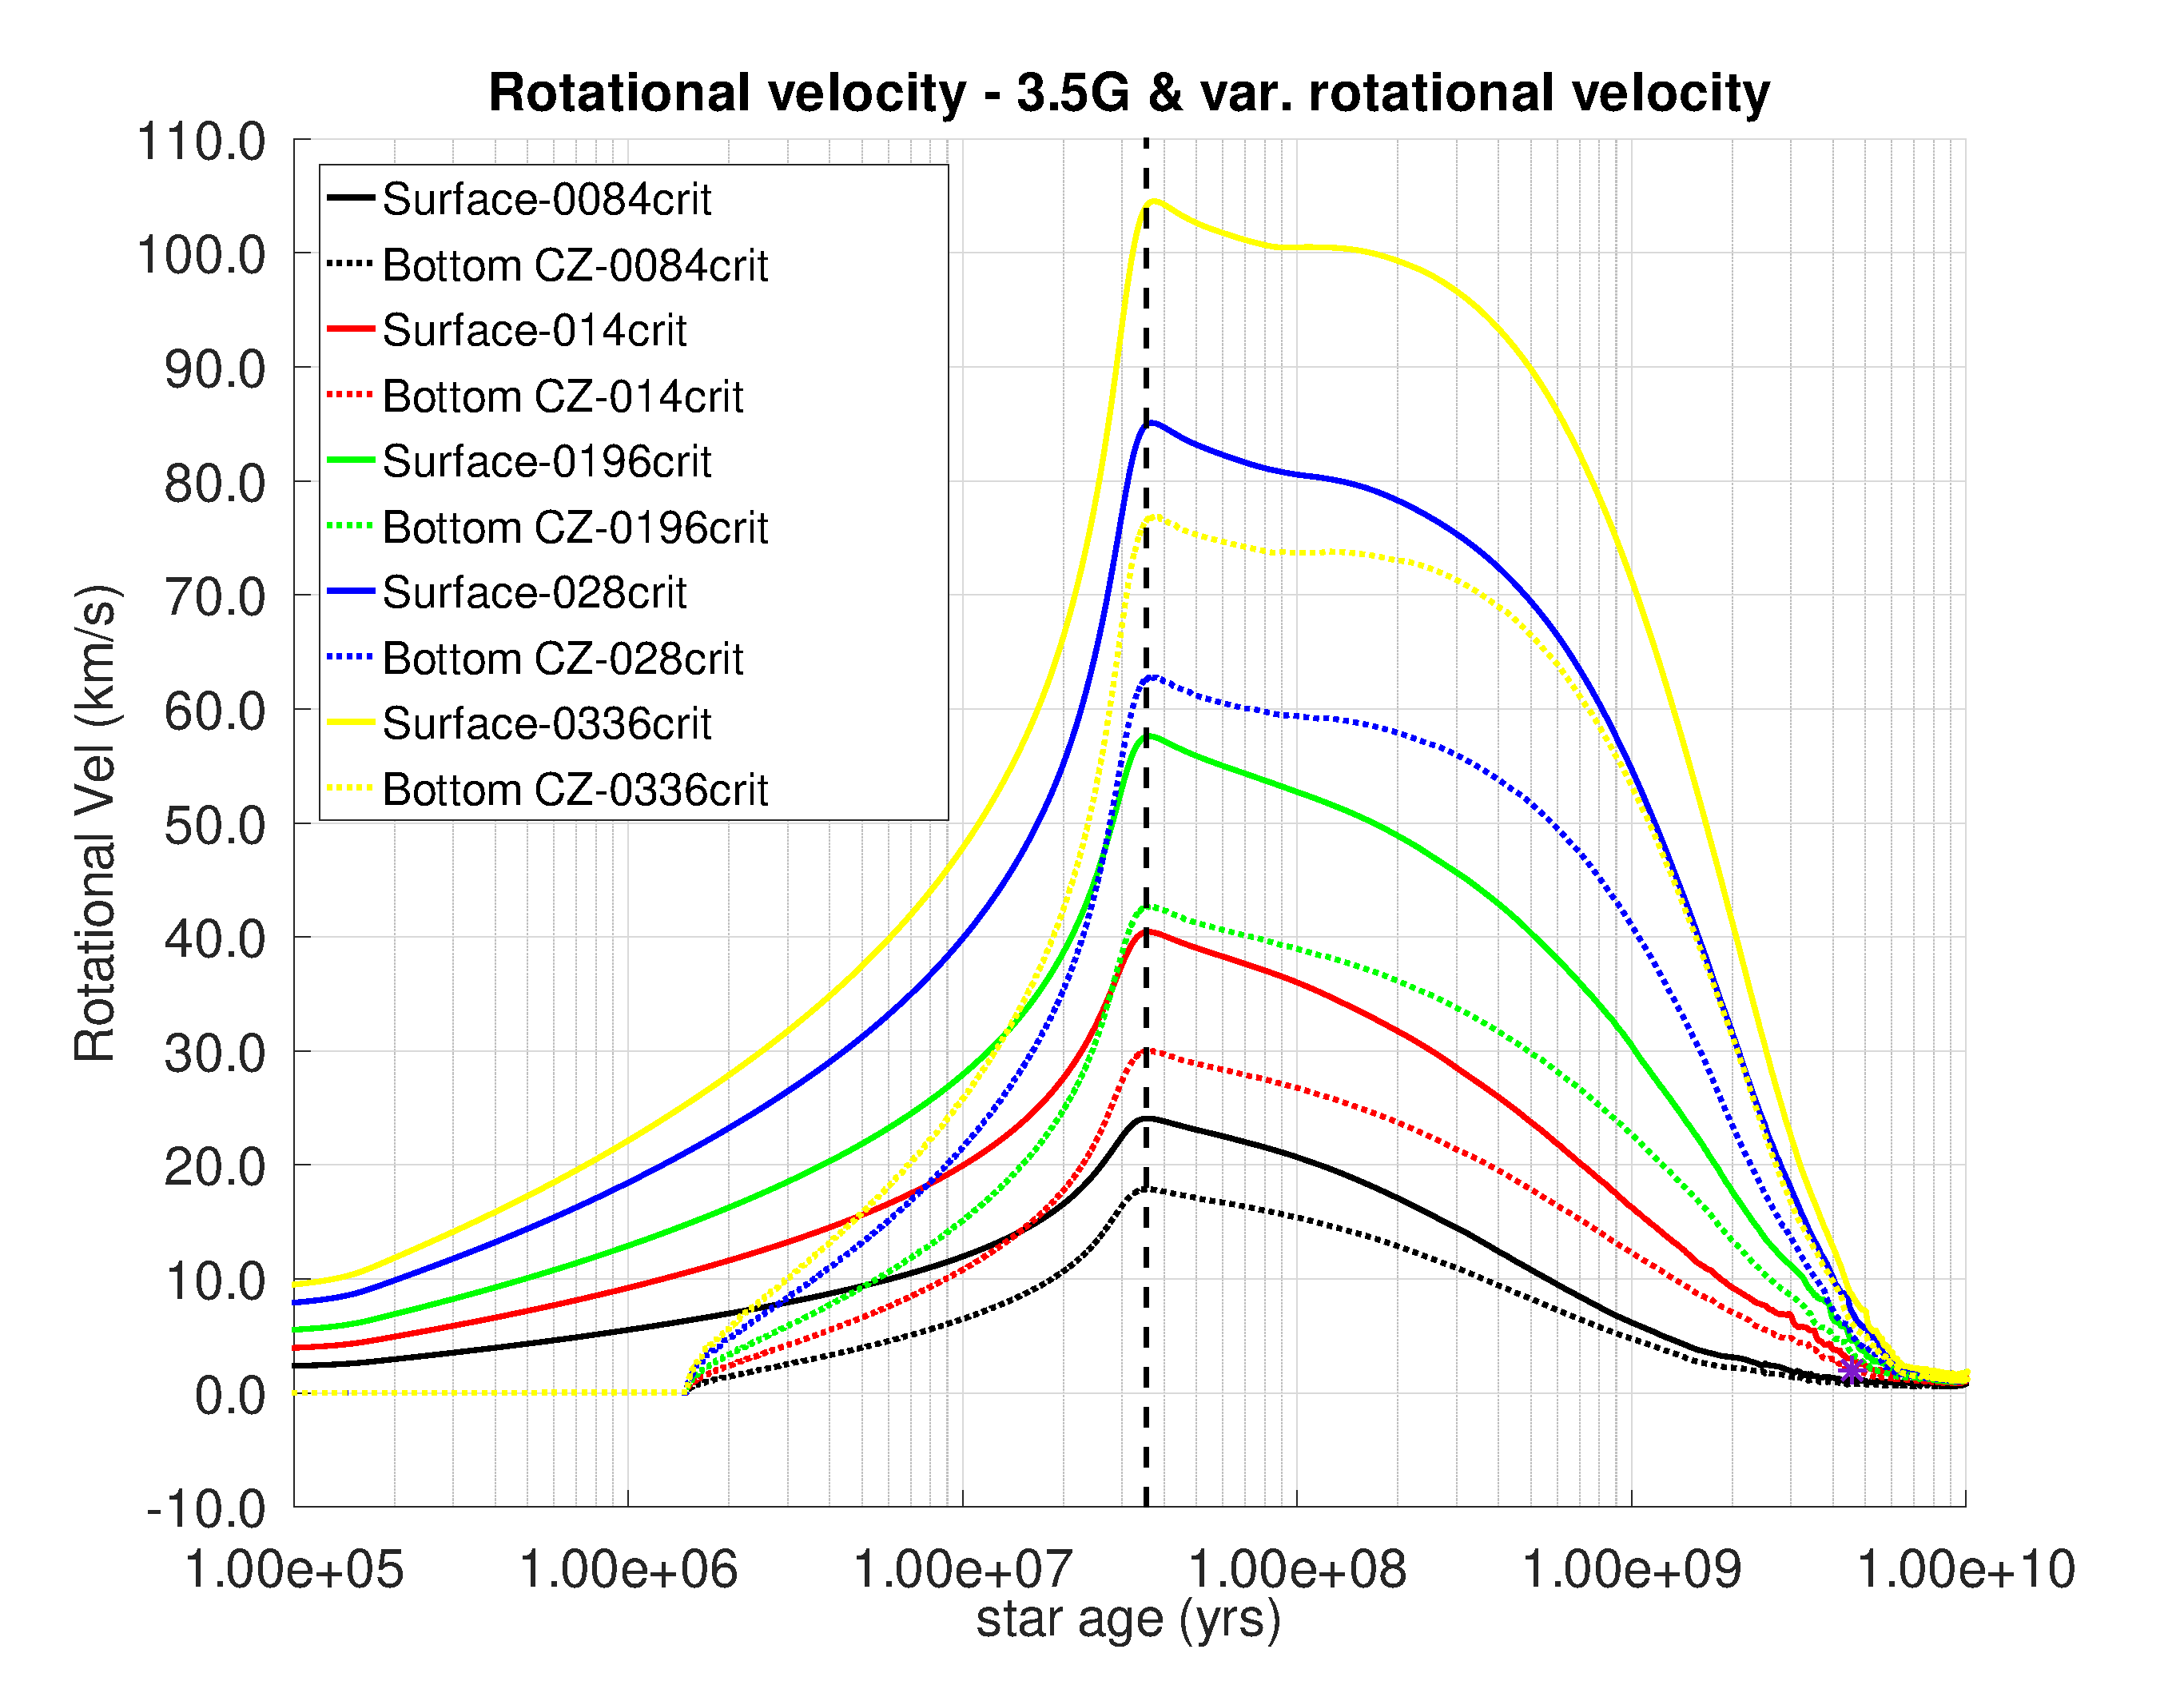
\includegraphics[trim = 30mm 15mm 20mm 15mm, clip,width=\textwidth]{figures/rot_vel_var_vel_3_5g.eps}
    \label{fig:subim42}
    \end{subfigure}
    \begin{subfigure}[h]{0.47\textwidth}
    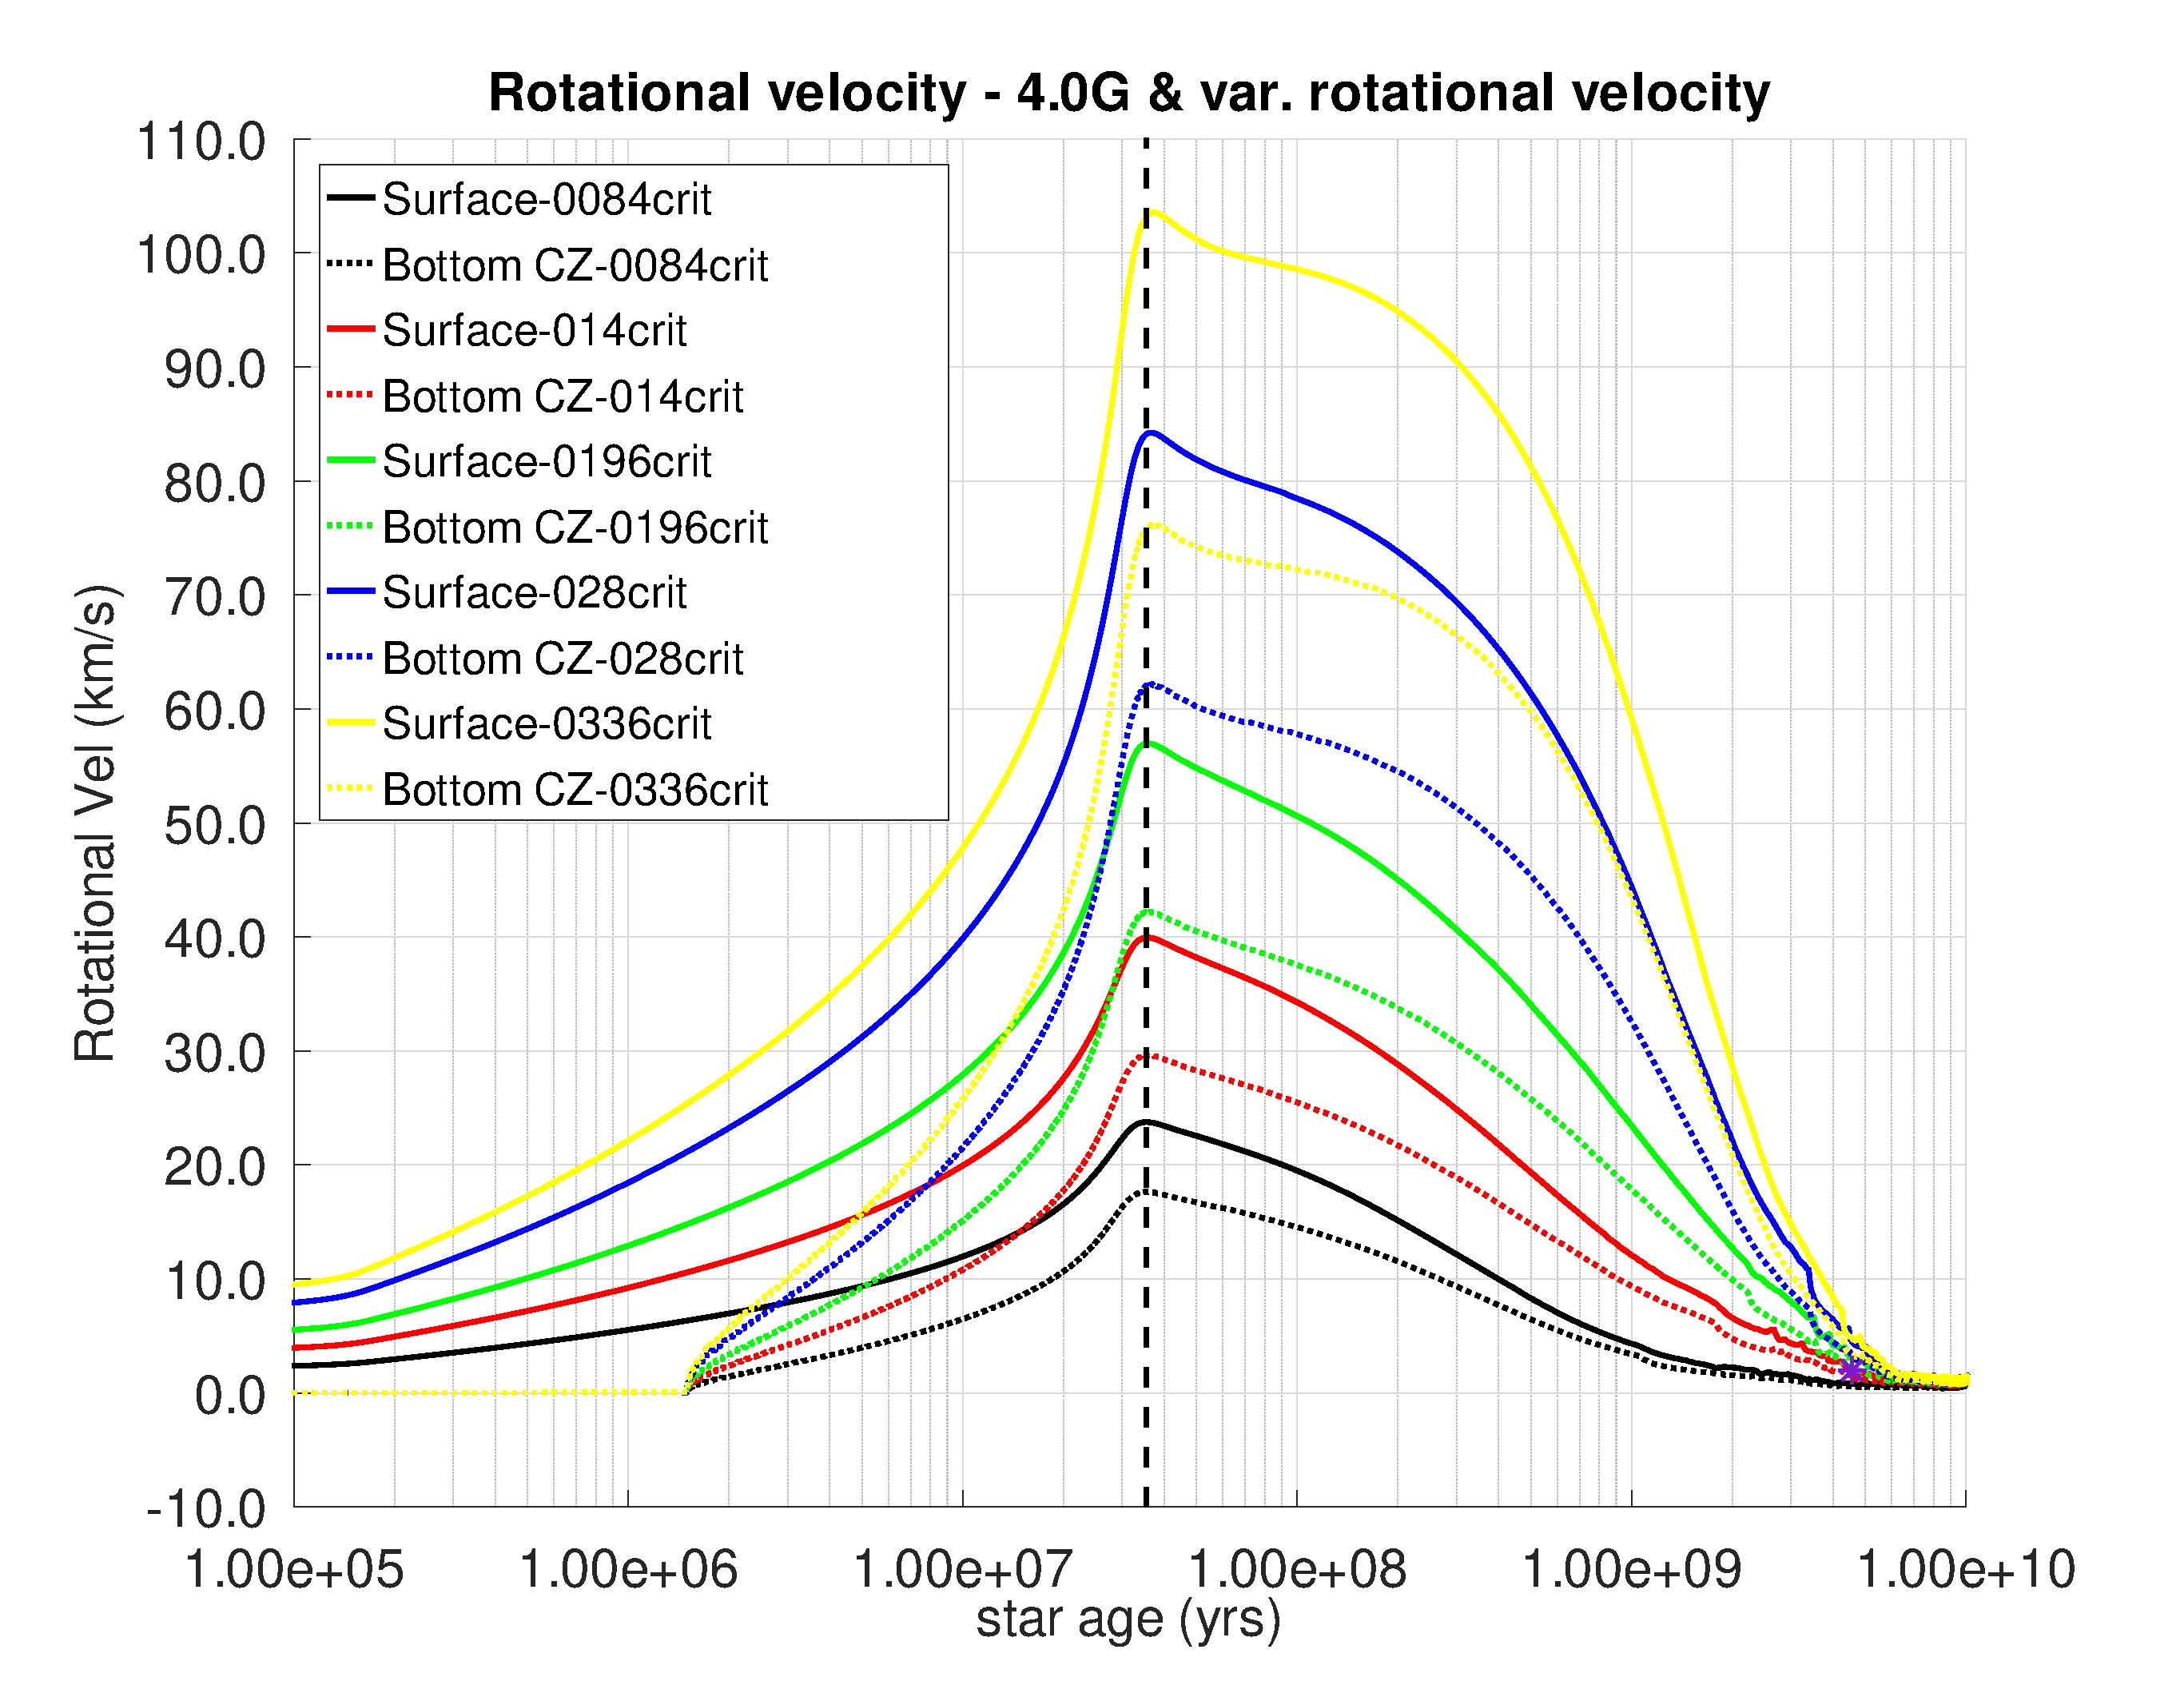
\includegraphics[trim = 30mm 15mm 20mm 15mm, clip,width=\textwidth]{figures/rot_vel_var_vel_4_0g.eps}
    \label{fig:subim43}
    \end{subfigure}
    \begin{subfigure}[h]{0.47\textwidth}
    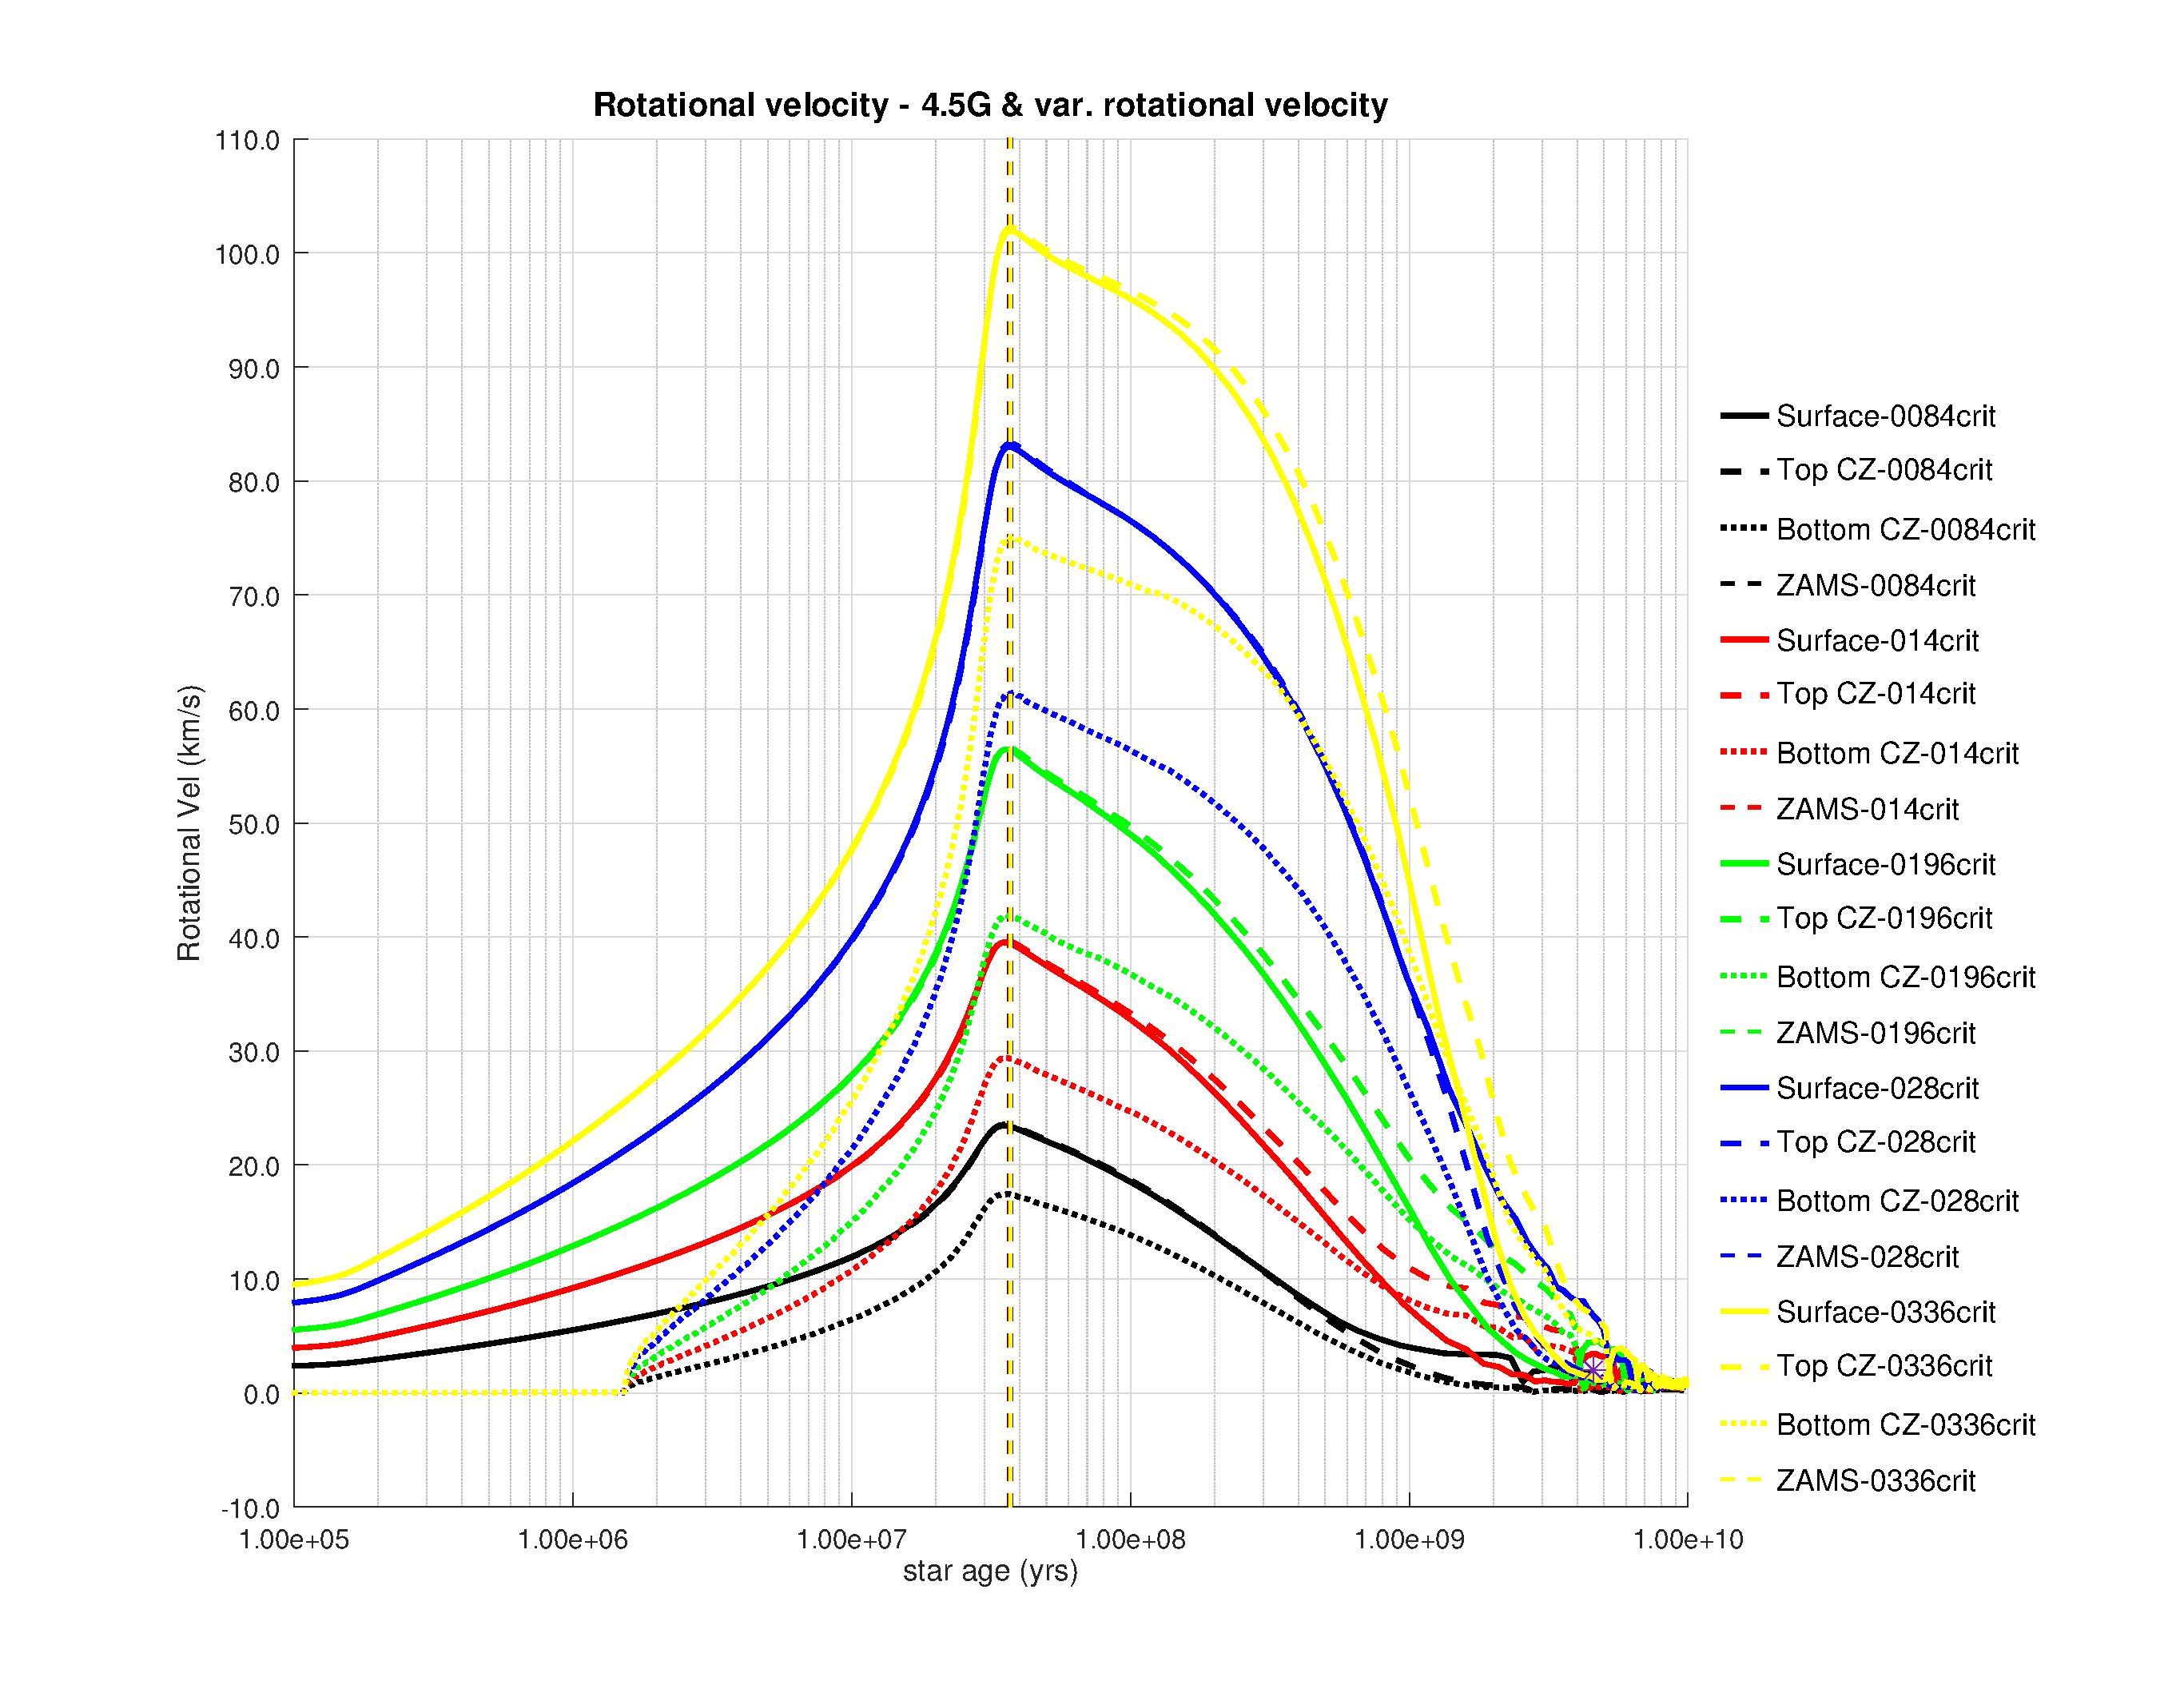
\includegraphics[trim = 30mm 15mm 20mm 15mm, clip,width=\textwidth]{figures/rot_vel_var_vel_4_5g.eps}
    \label{fig:subim44}
    \end{subfigure}
    \begin{subfigure}[h]{0.47\textwidth}
    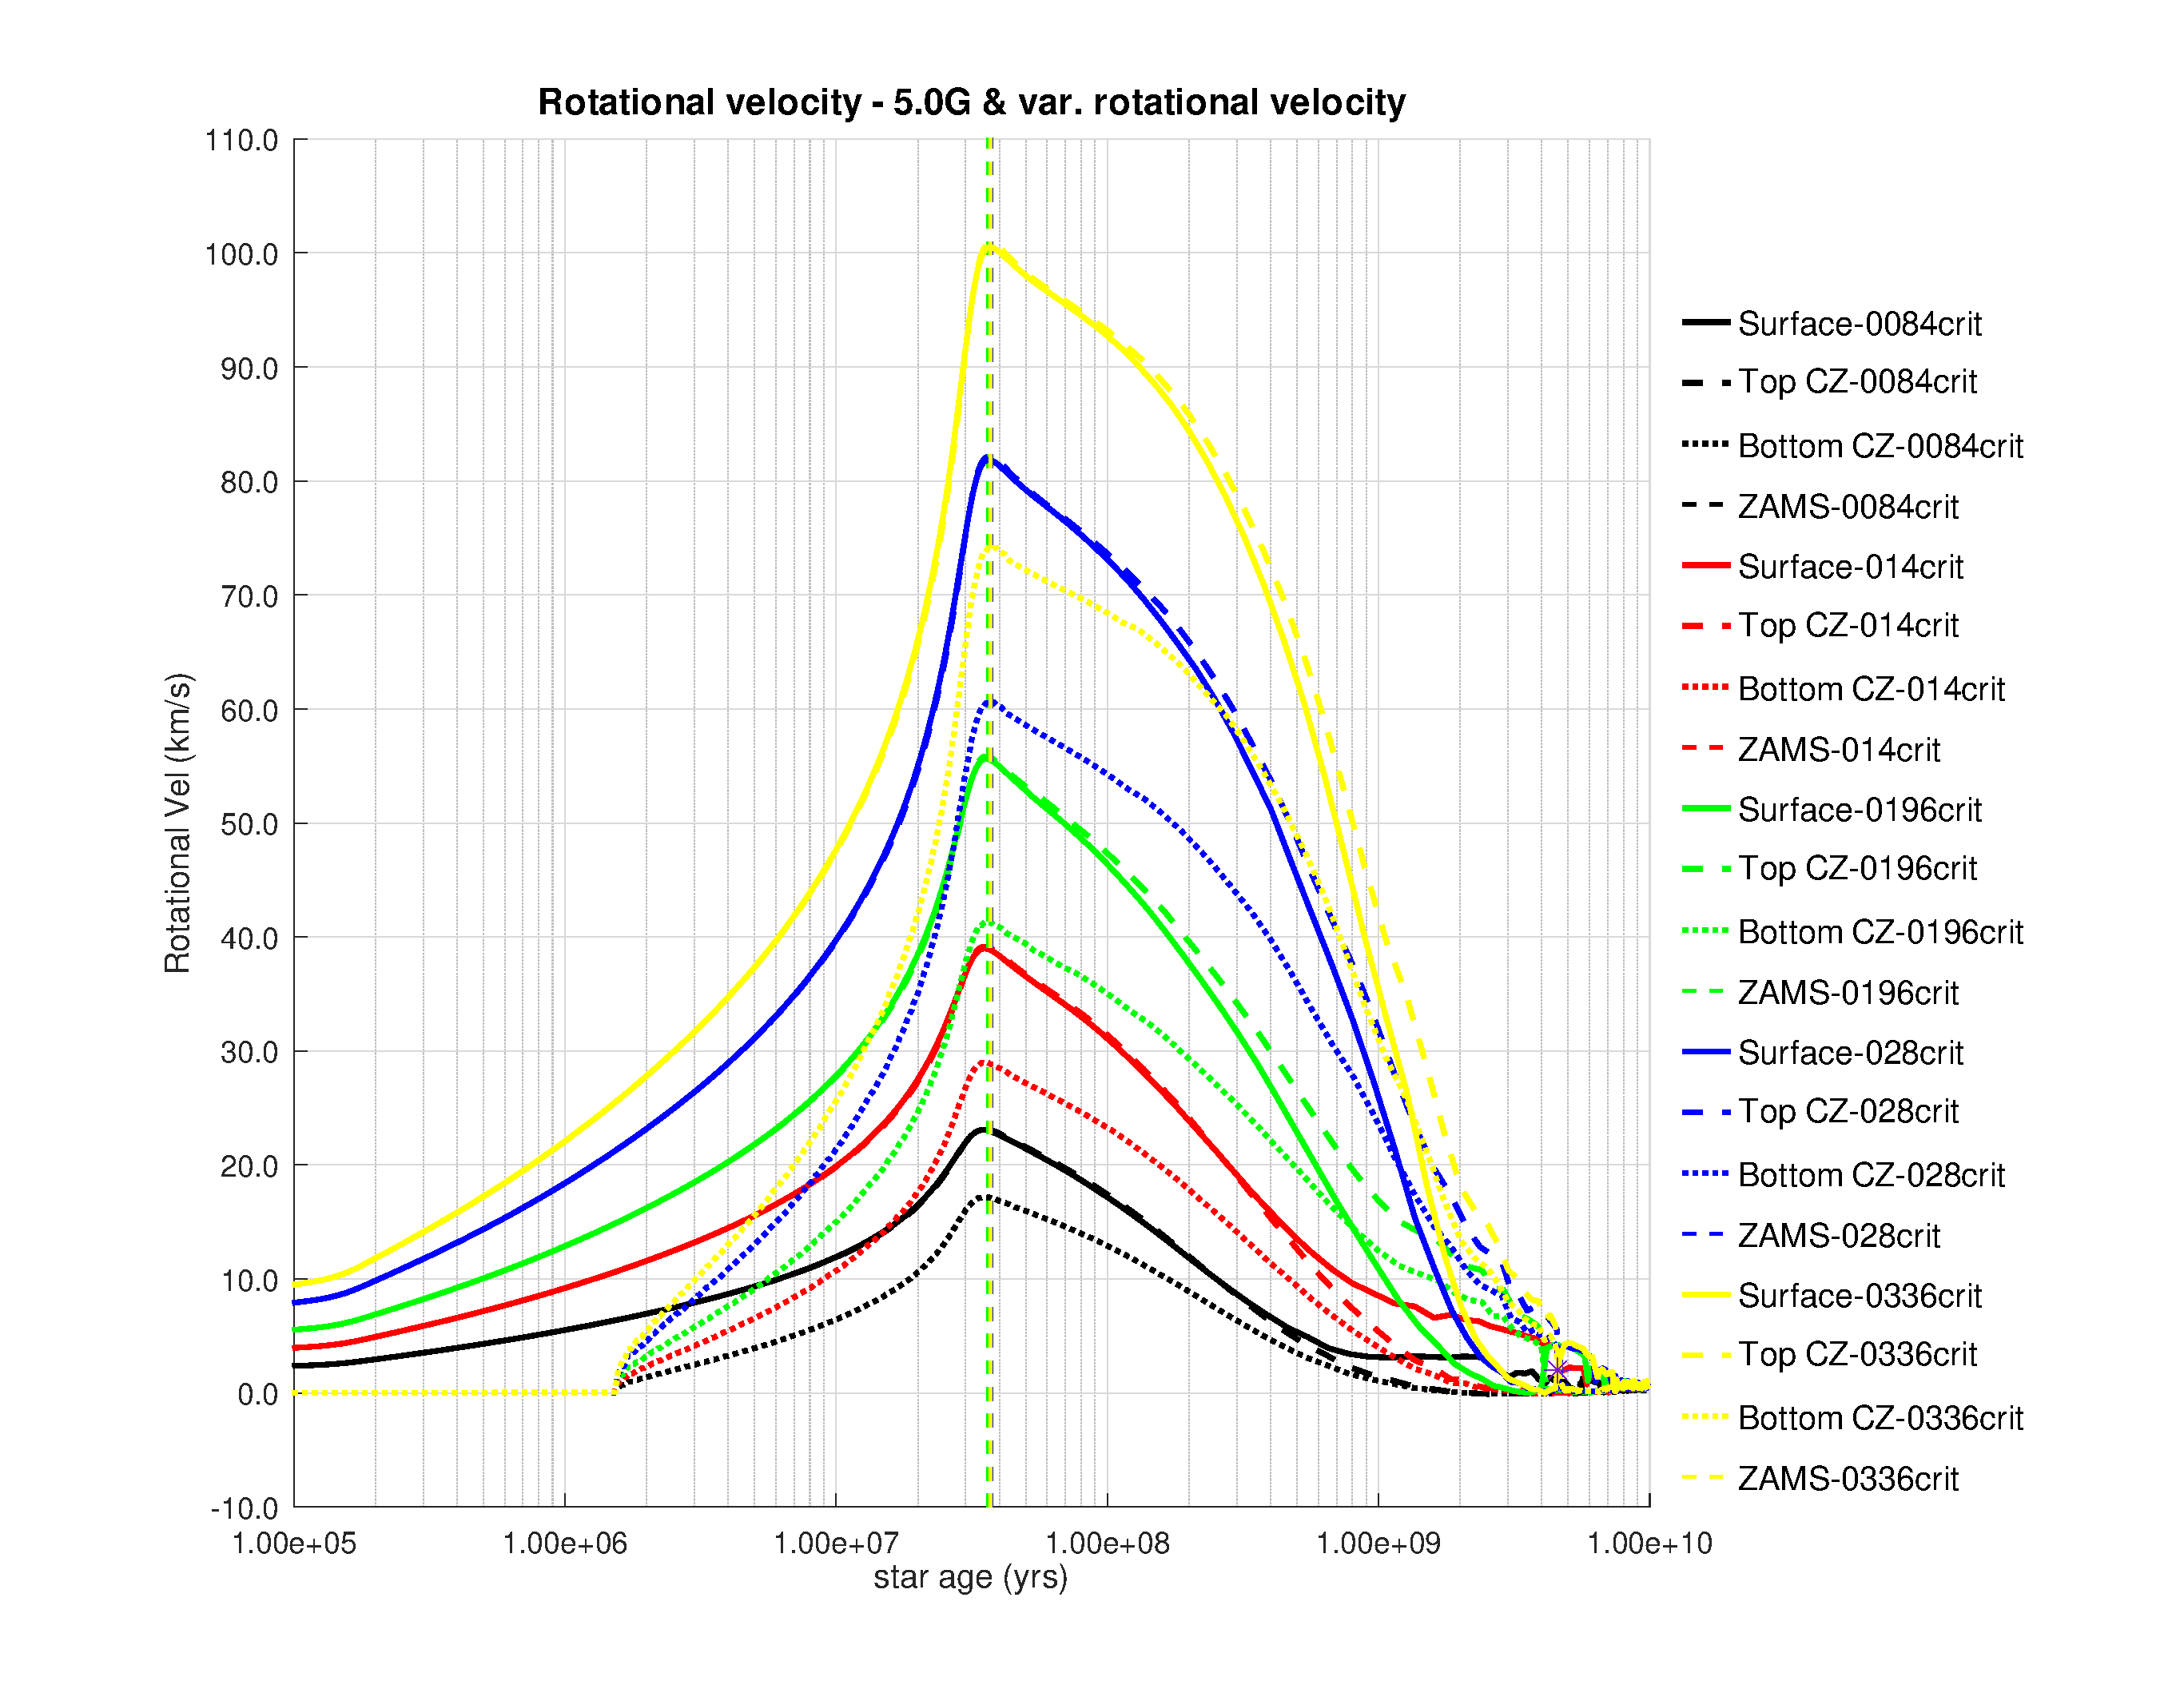
\includegraphics[trim = 30mm 15mm 20mm 15mm, clip,width=\textwidth]{figures/rot_vel_var_vel_5_0g.eps}
    \label{fig:subim45}
    \end{subfigure}
    \begin{subfigure}[h]{0.47\textwidth}
    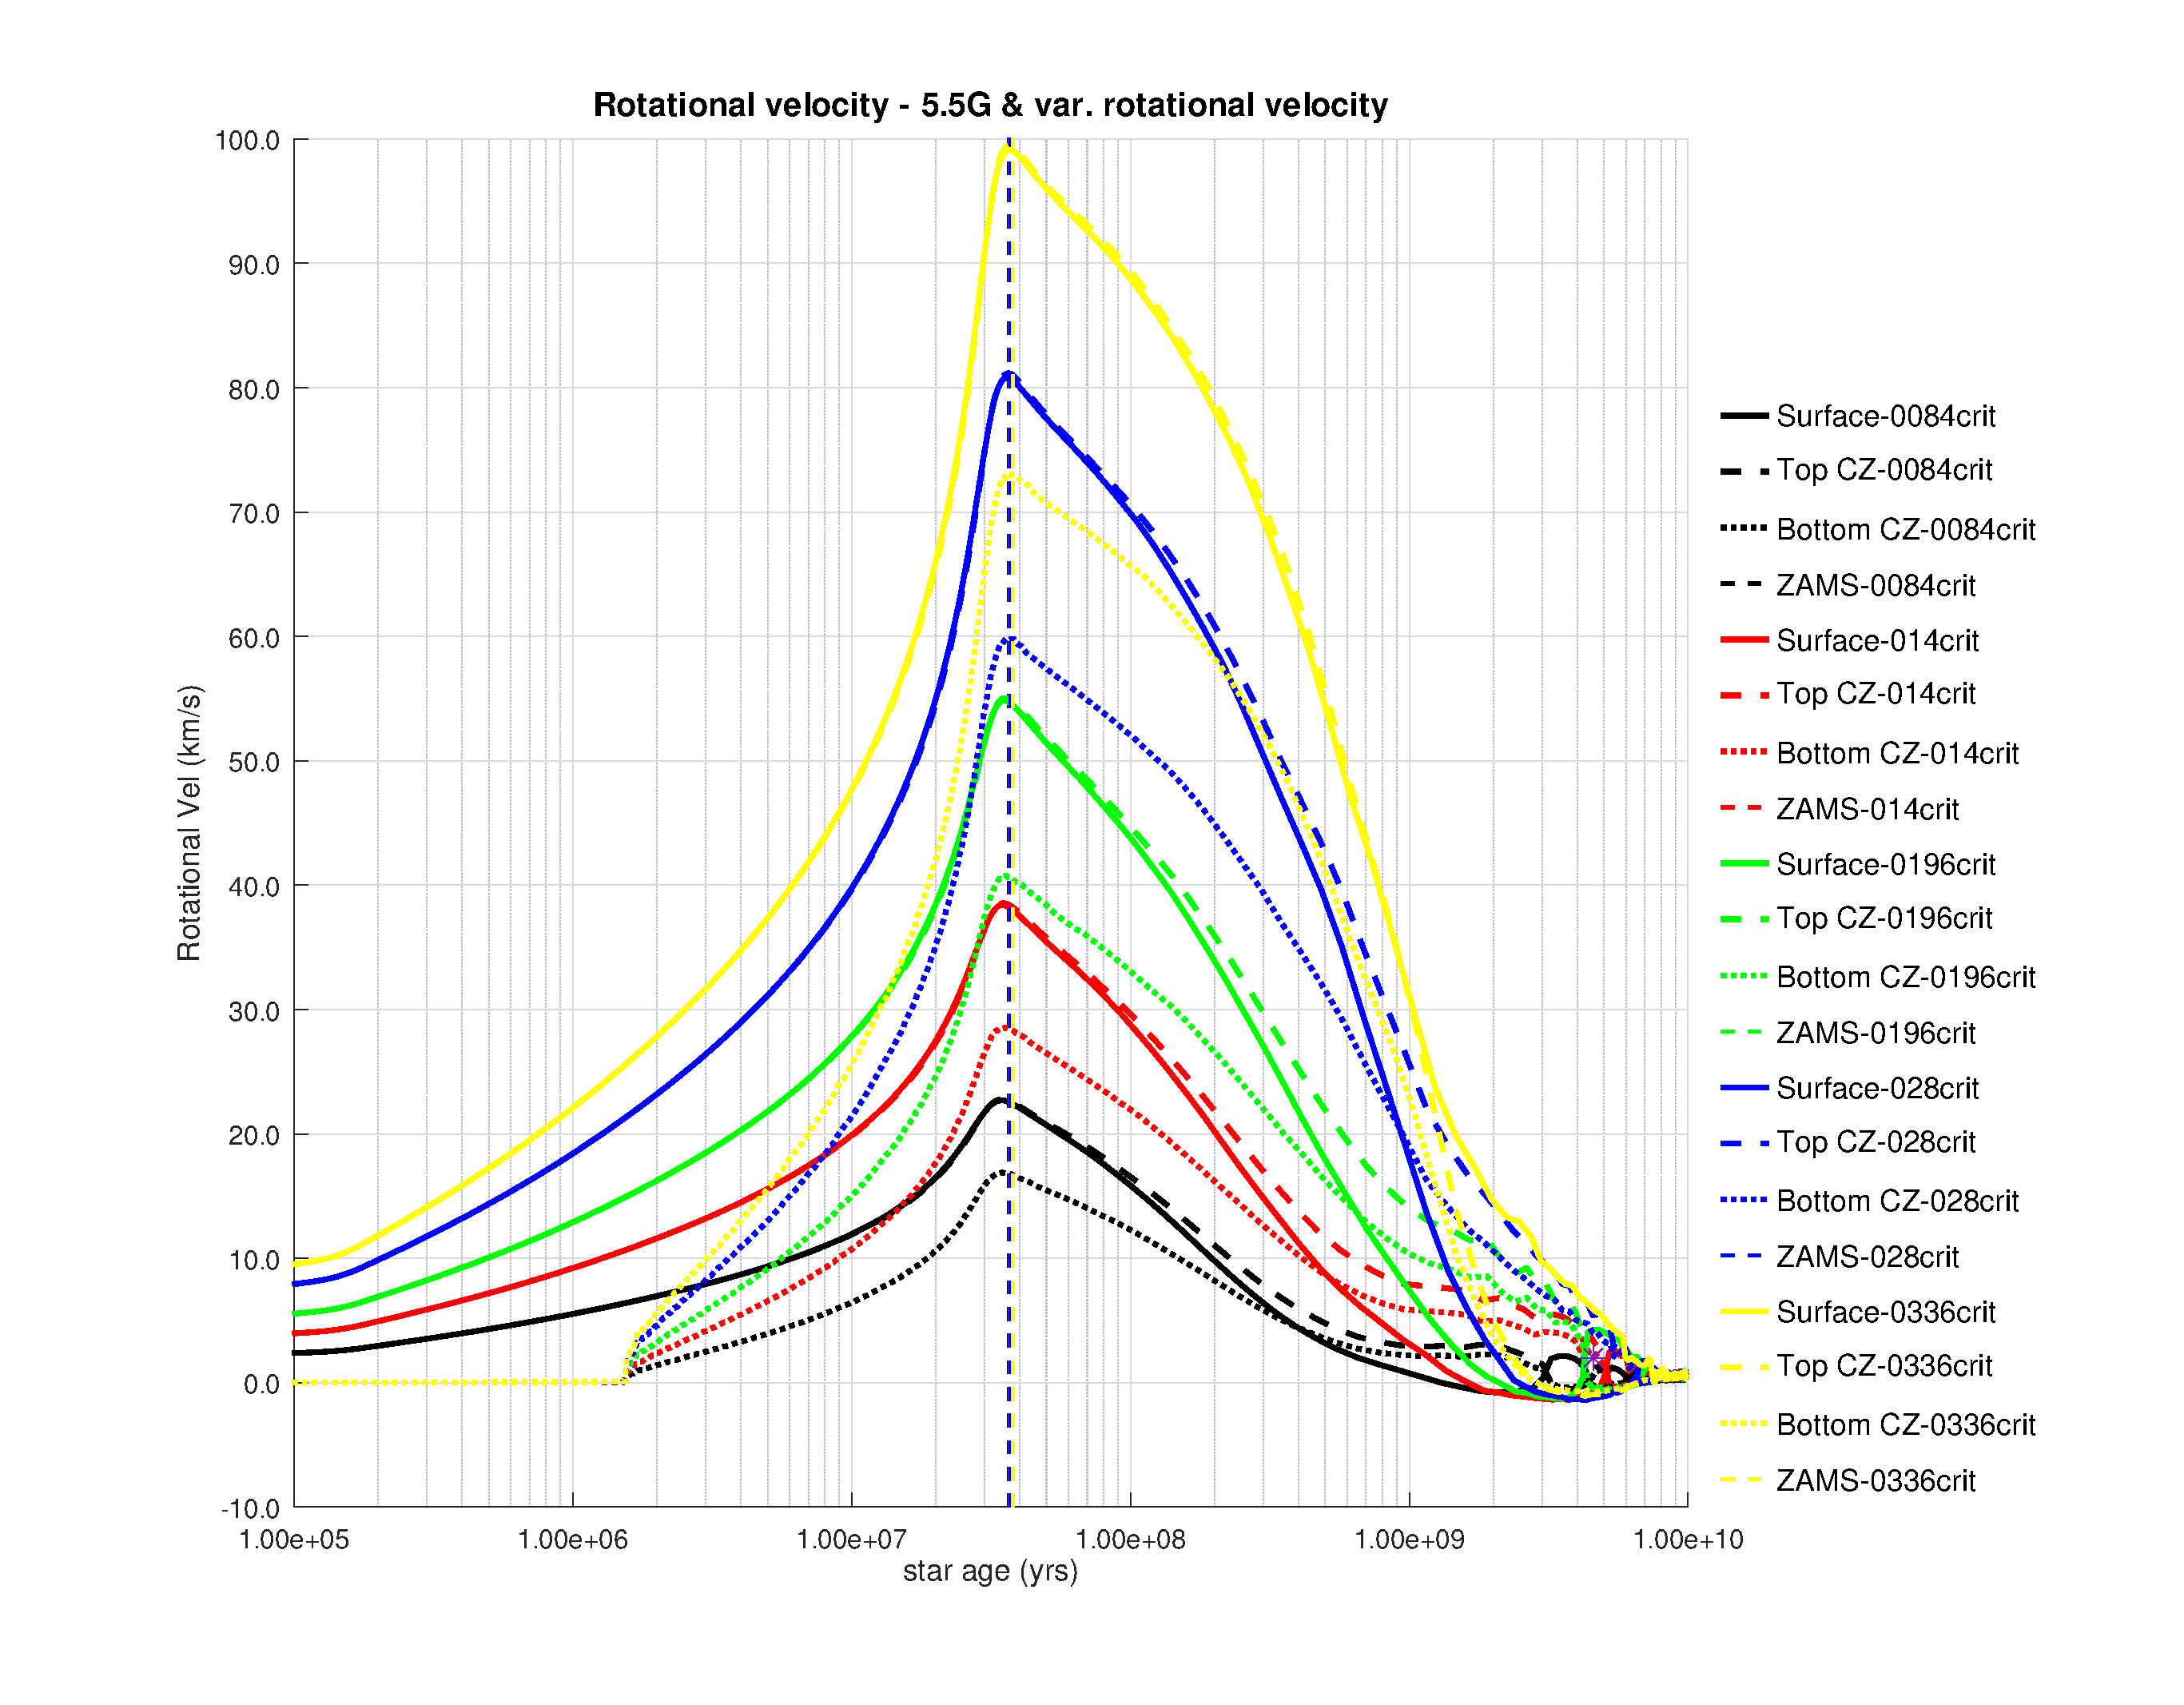
\includegraphics[trim = 30mm 15mm 20mm 15mm, clip,width=\textwidth]{figures/rot_vel_var_vel_5_5g.eps}
    \label{fig:subim46}
    \end{subfigure}
\caption{Grid showing the evolution of the evolution of surface rotational velocity, as a function of time for several 1 $M_{\sun}$ models. Each figure shows a set of models in which the magnetic field with intensity has been fixed and $\Omega / \Omega_{crit}$ varies between 0.0084 and 0.0336. The purple star is the surface angular velocity for the present-day Sun \citep{Gill2012}. The dashed lines make reference to the ZAMS.}
\label{fig:grid_rot_vel}
\end{figure*}




\begin{figure*}
    \centering
    \begin{subfigure}[h]{0.47\textwidth}
    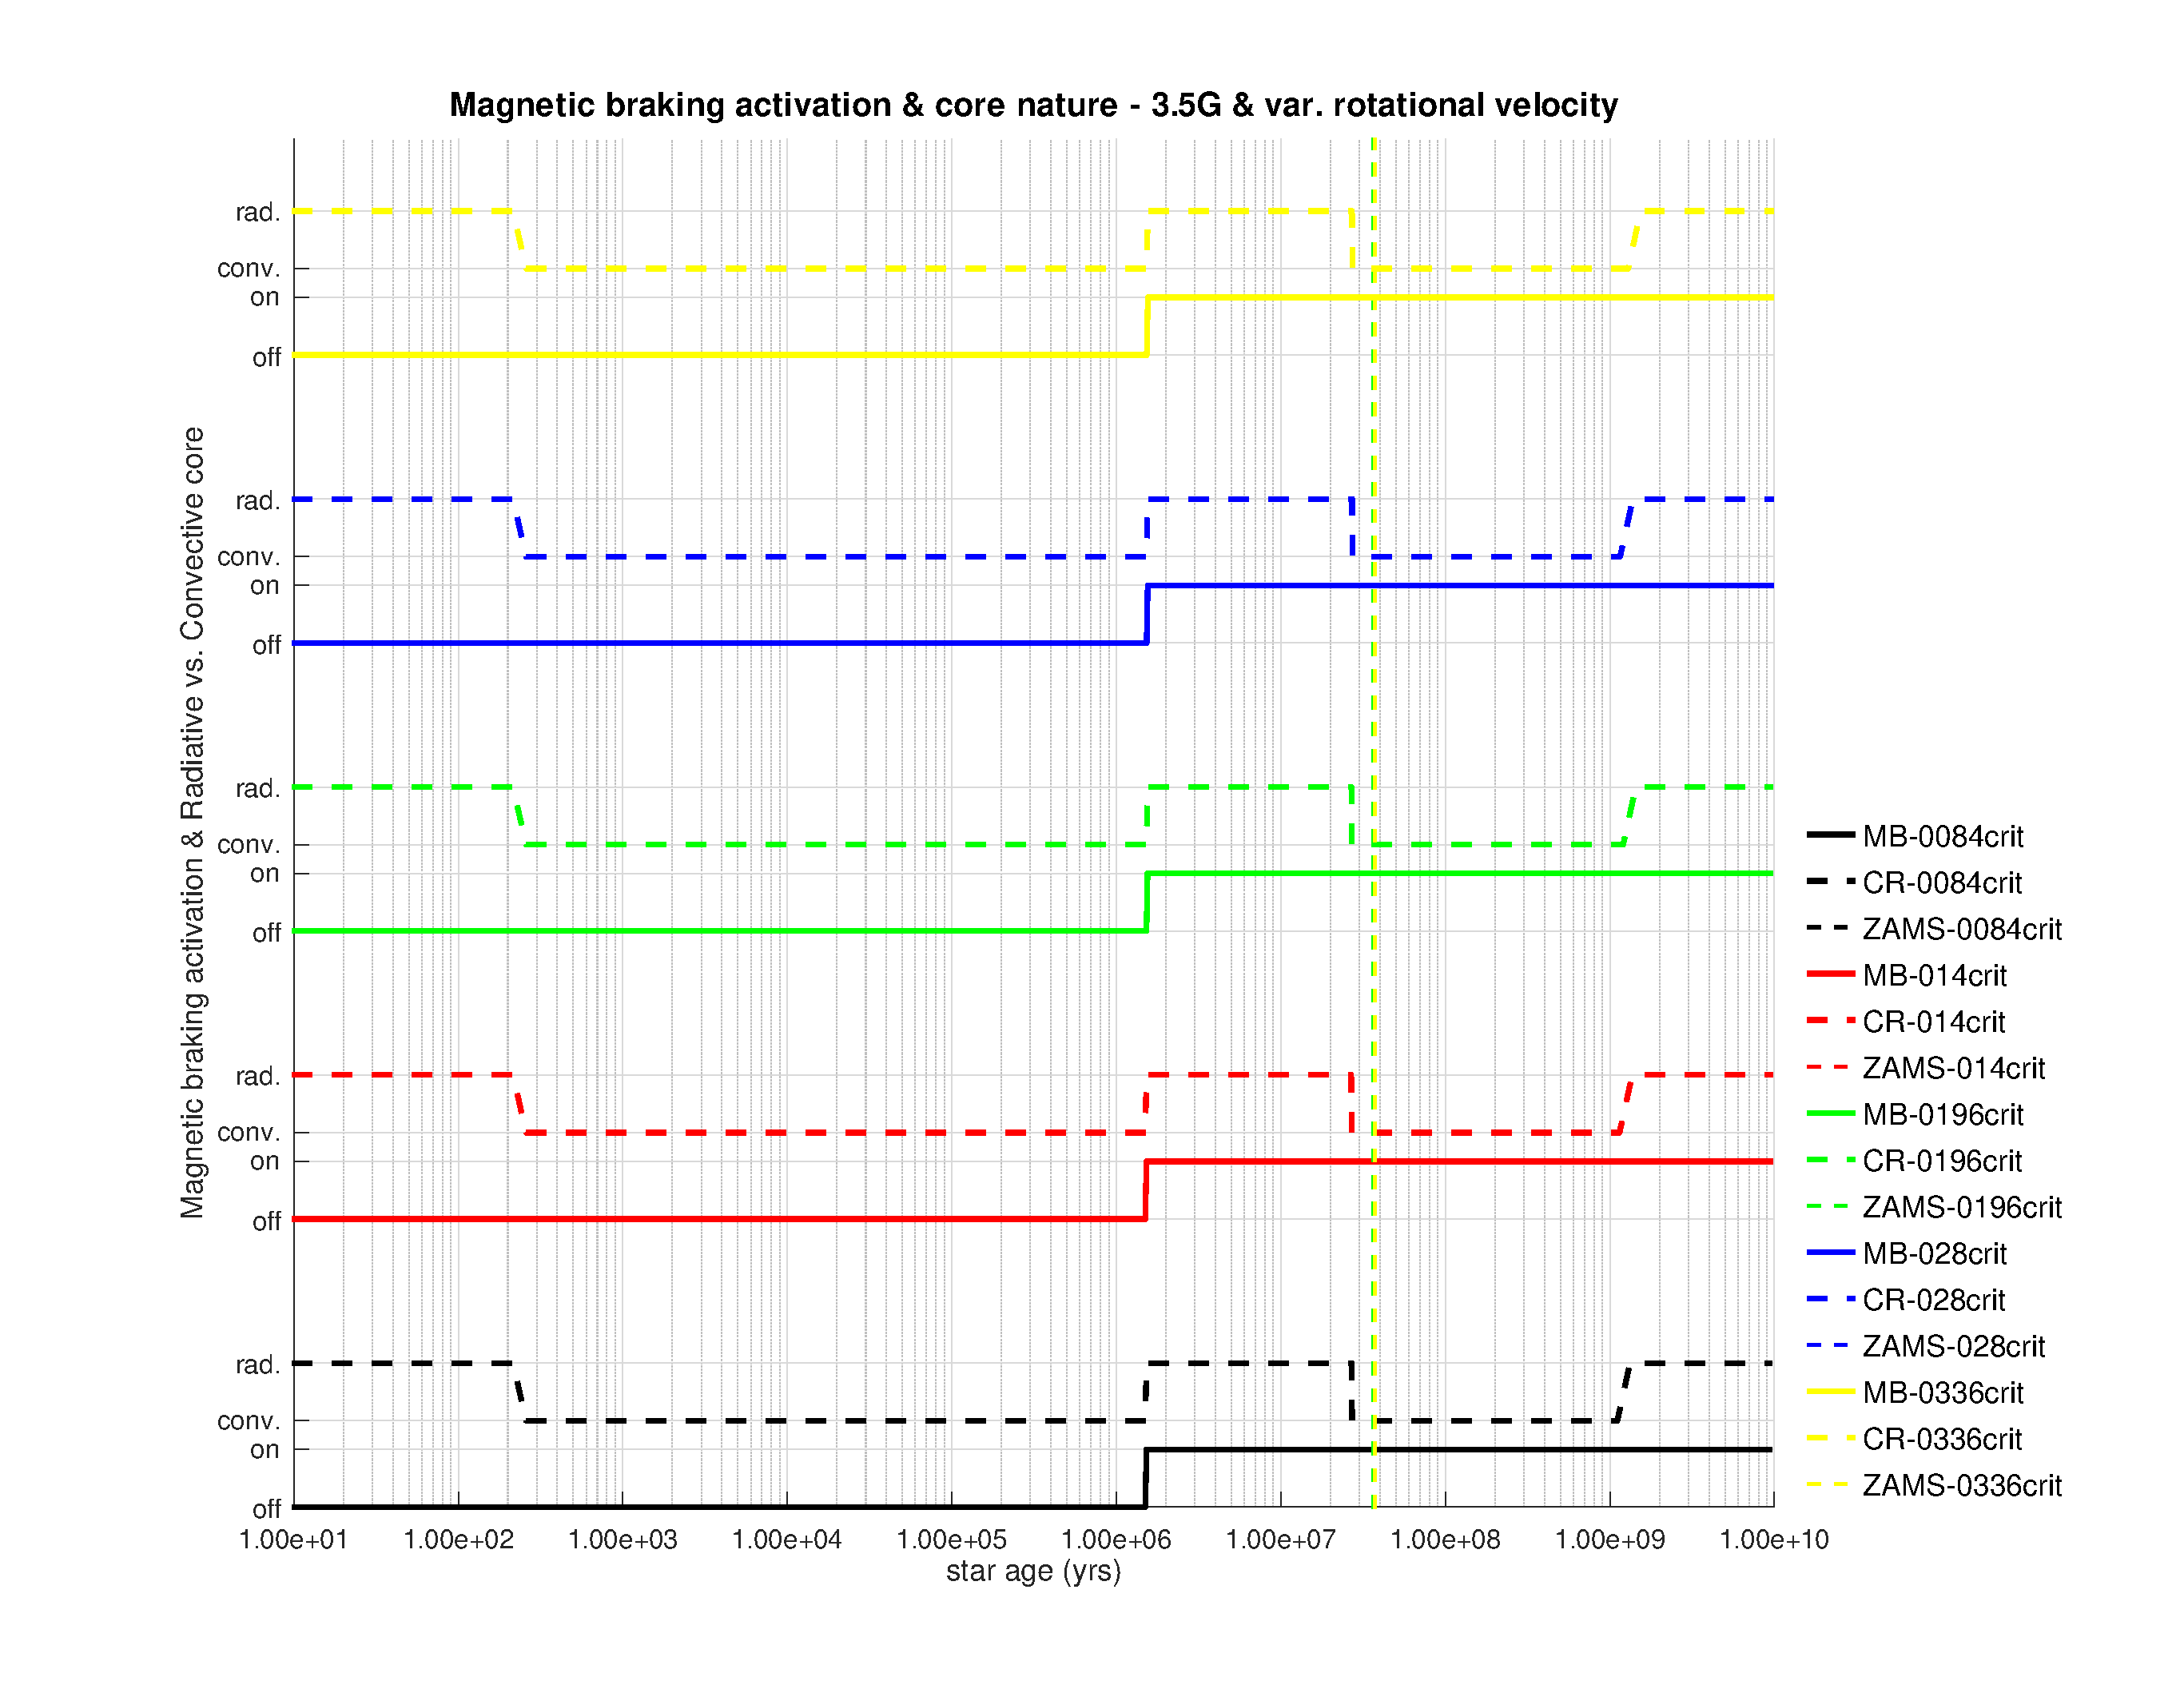
\includegraphics[trim = 30mm 15mm 20mm 15mm, clip,width=\textwidth]{figures/mb_act_var_vel_3_5g.eps}
    \label{fig:subim31}
    \end{subfigure}
    \begin{subfigure}[h]{0.47\textwidth}
    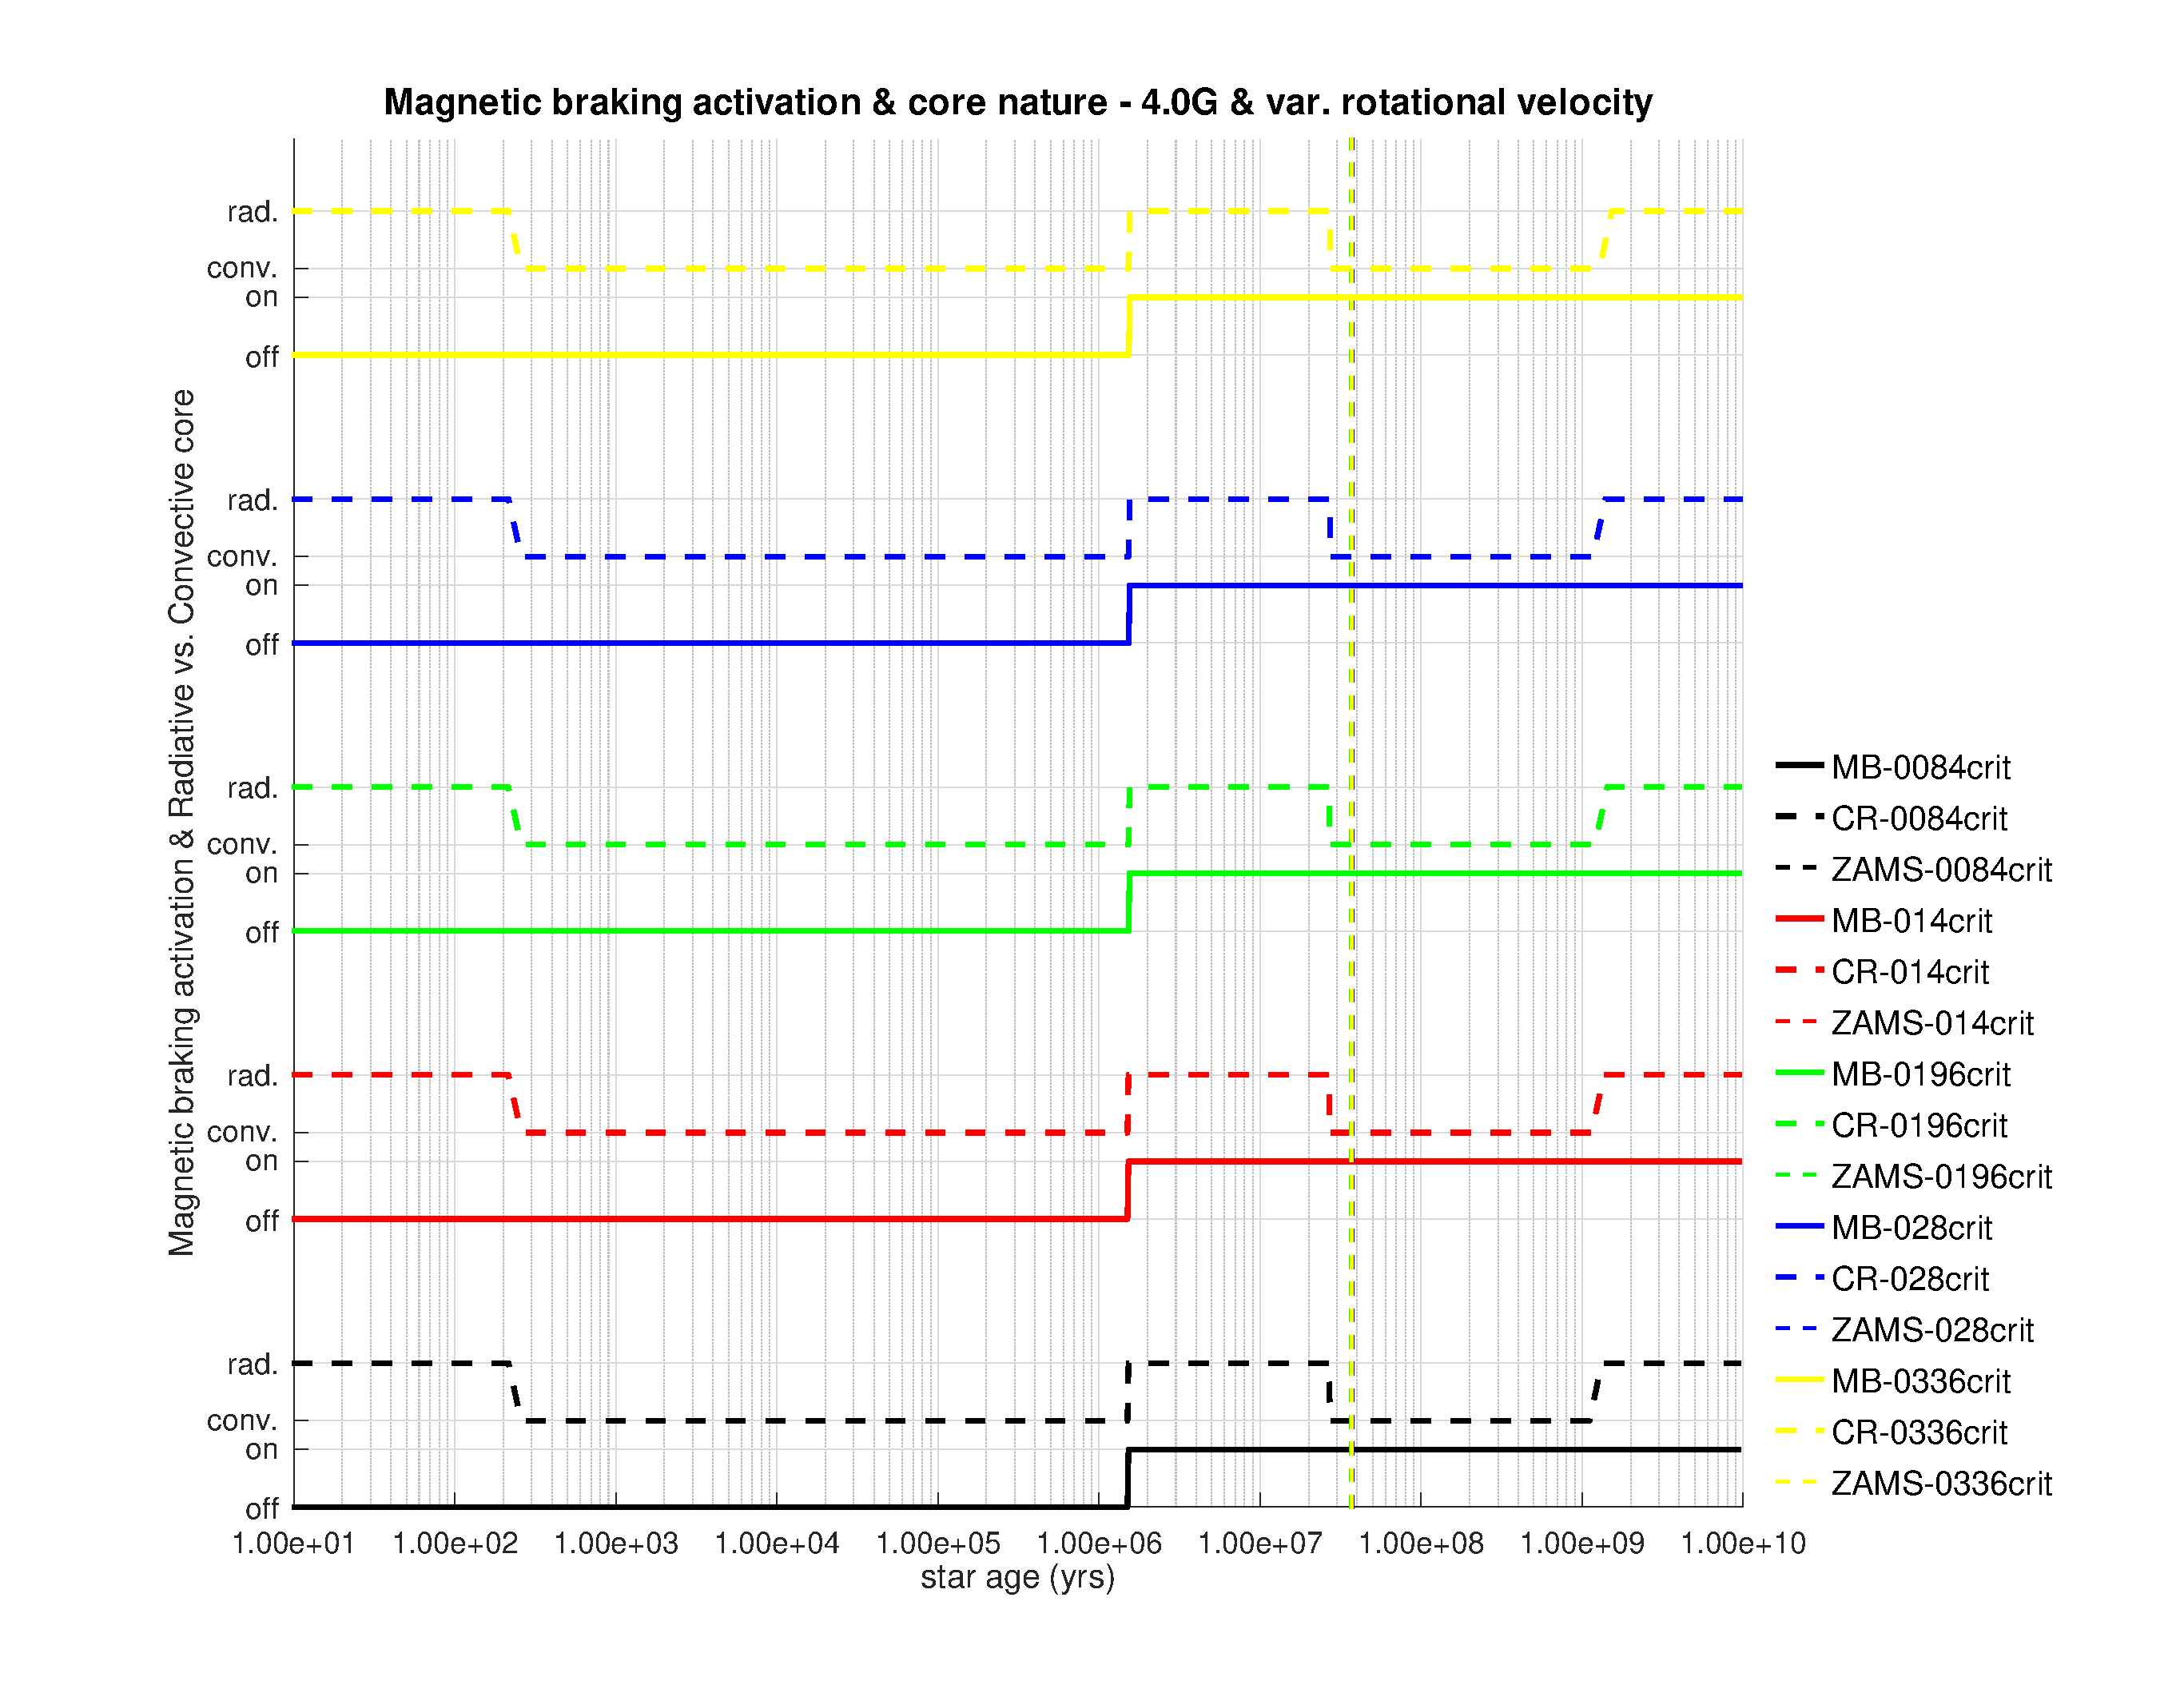
\includegraphics[trim = 30mm 15mm 20mm 15mm, clip,width=\textwidth]{figures/mb_act_var_vel_4_0g.eps}
    \label{fig:subim32}
    \end{subfigure}
    \begin{subfigure}[h]{0.47\textwidth}
    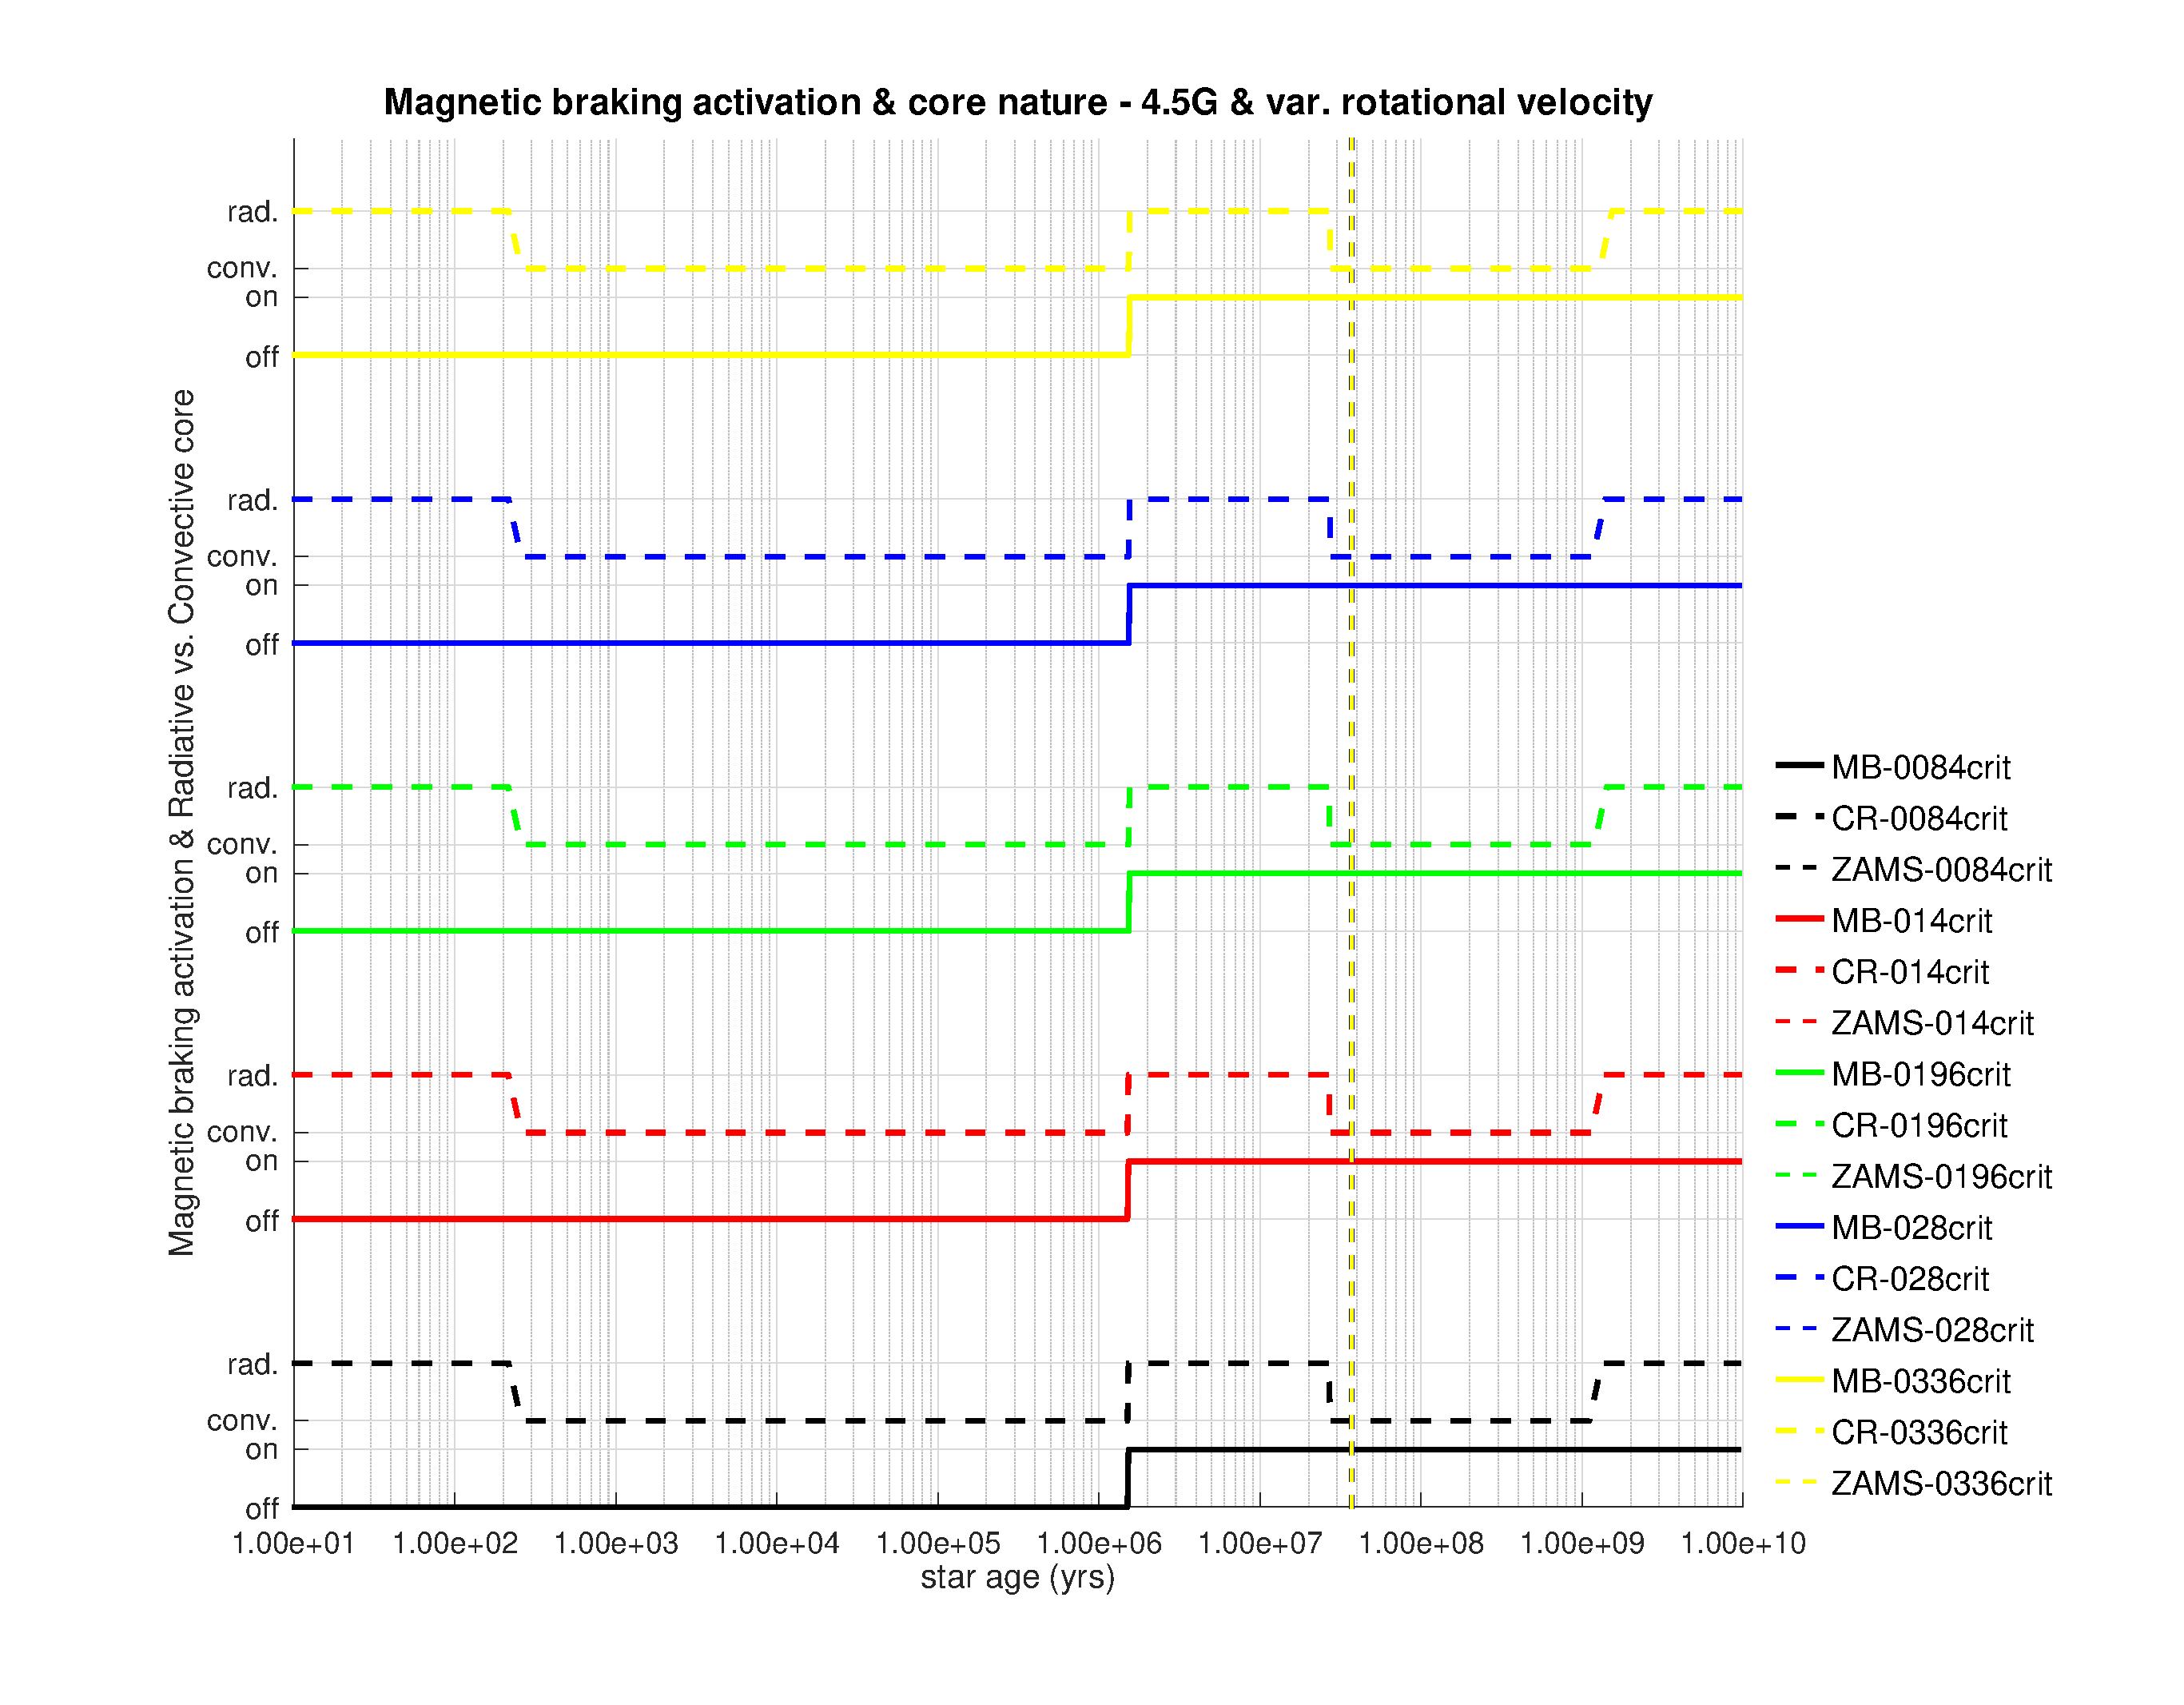
\includegraphics[trim = 30mm 15mm 20mm 15mm, clip,width=\textwidth]{figures/mb_act_var_vel_4_5g.eps}
    \label{fig:subim33}
    \end{subfigure}
    \begin{subfigure}[h]{0.47\textwidth}
    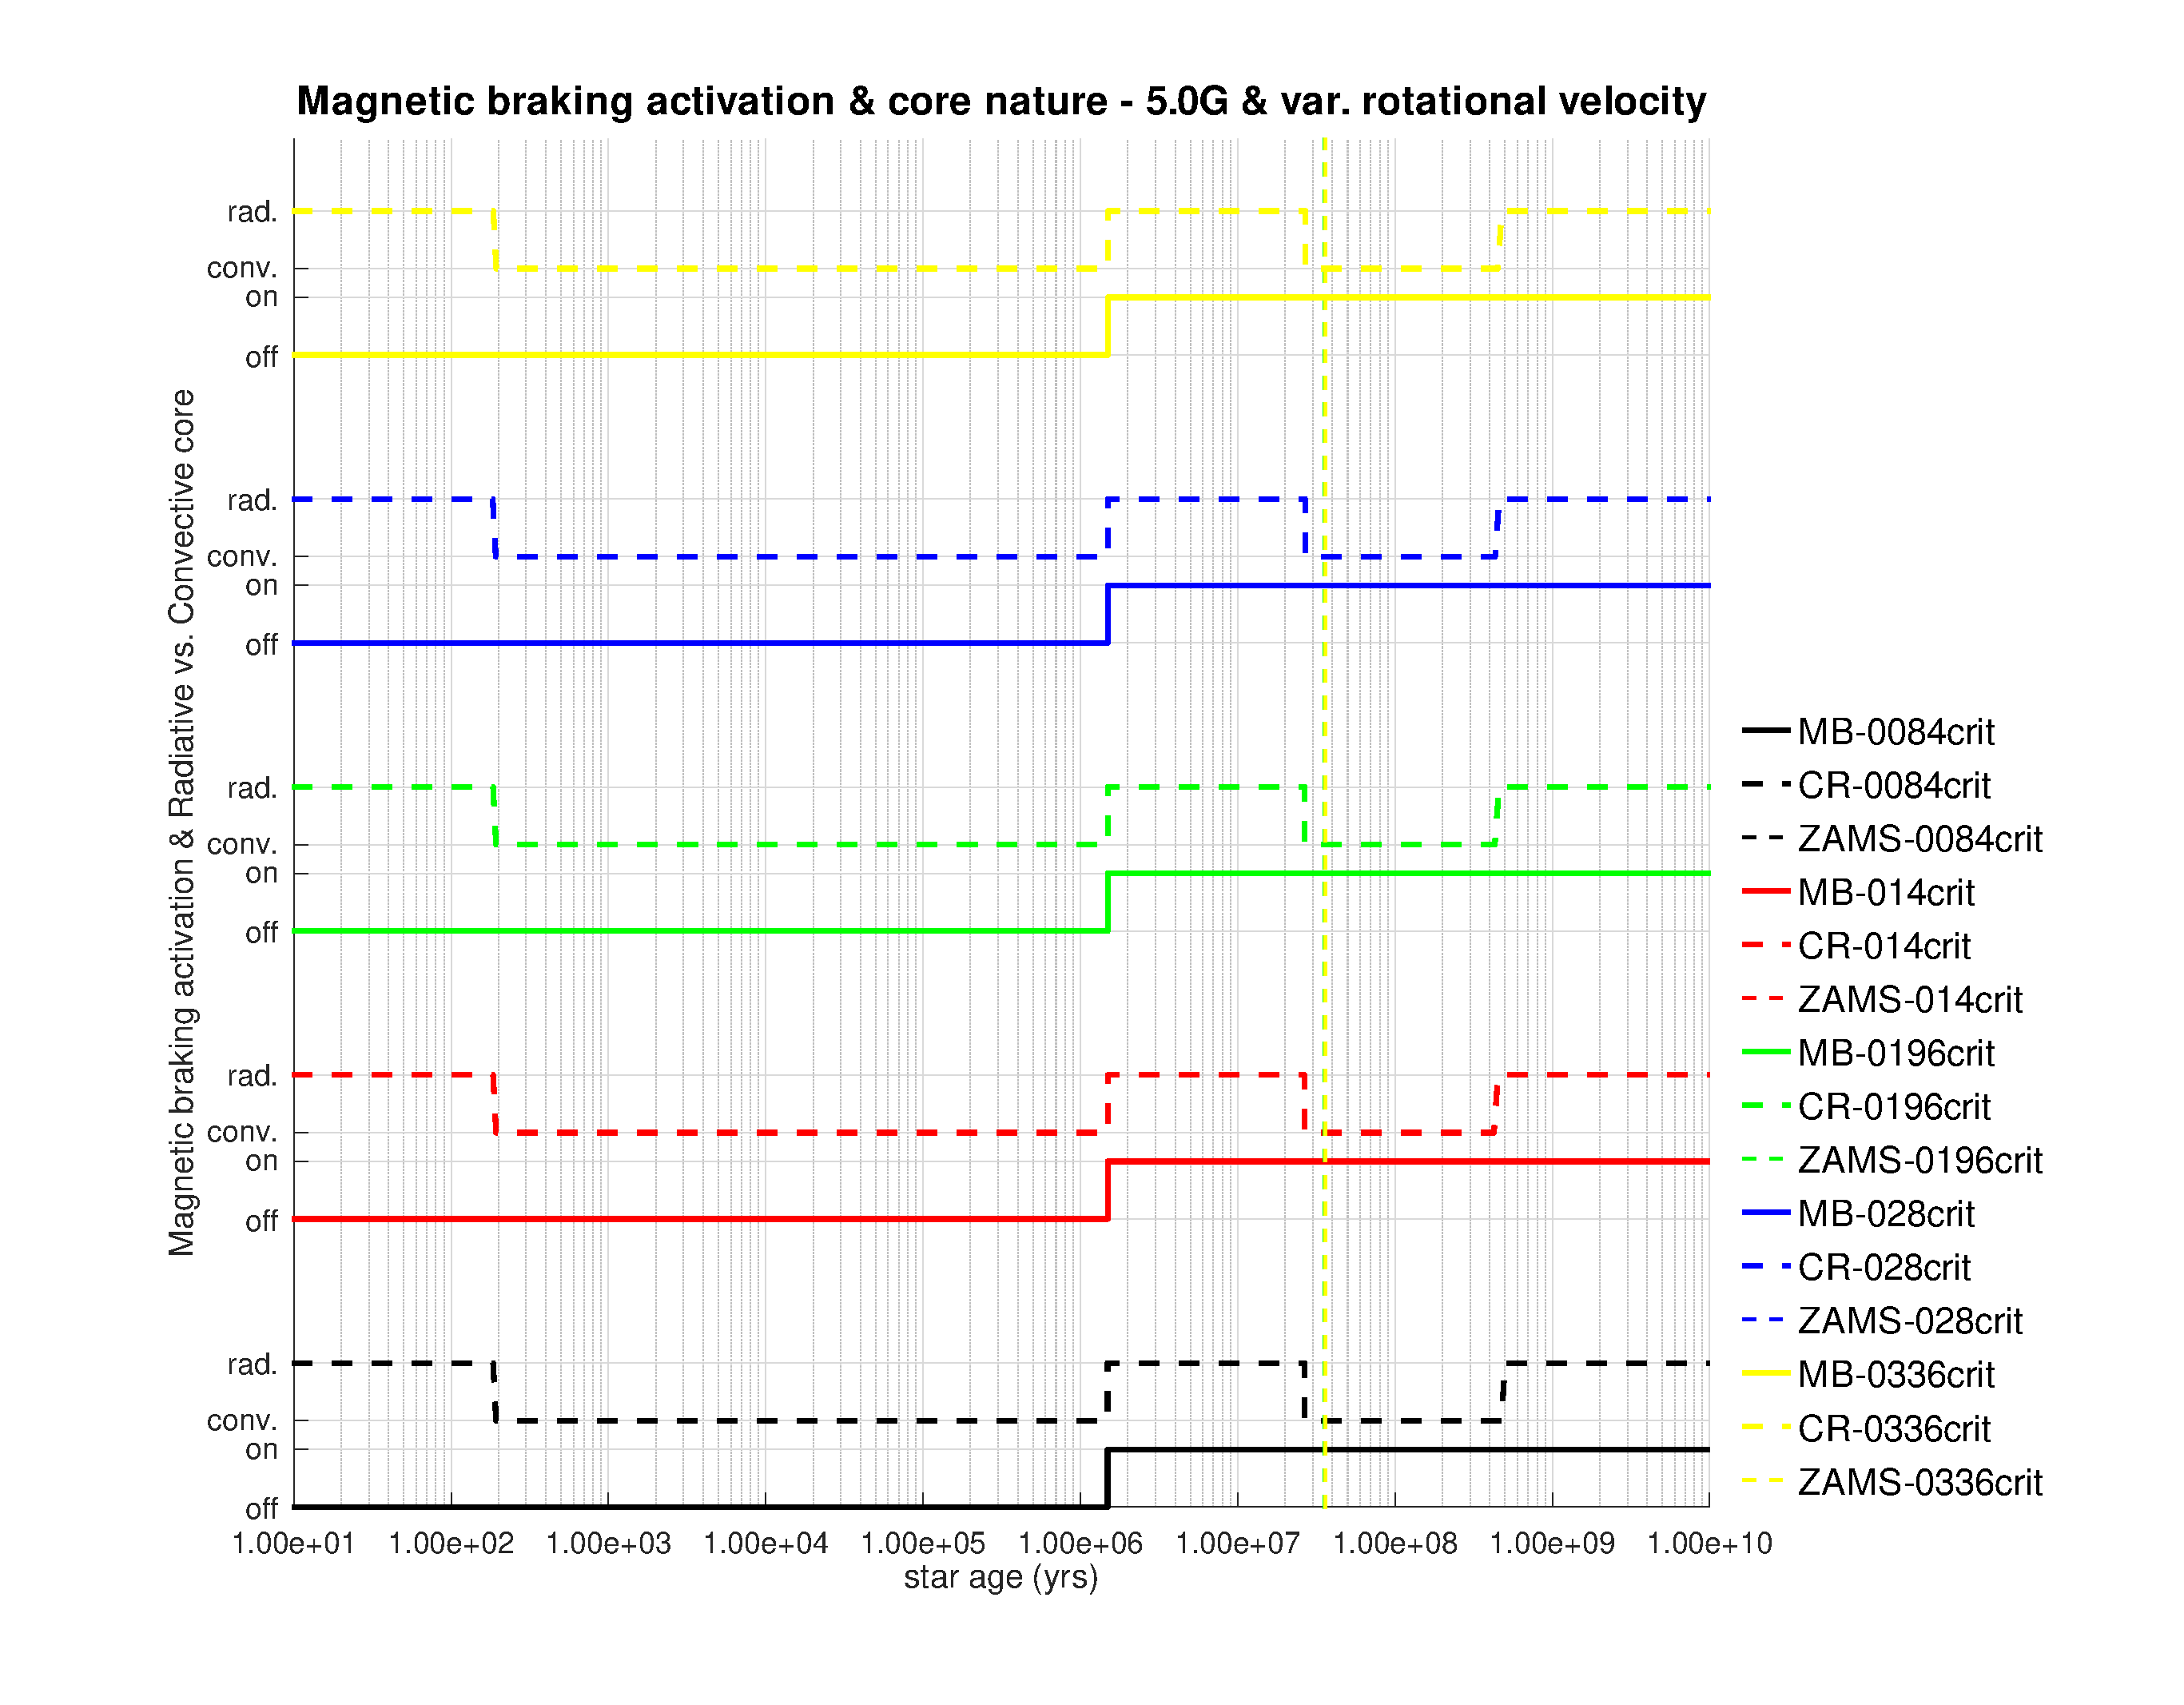
\includegraphics[trim = 30mm 15mm 20mm 15mm, clip,width=\textwidth]{figures/mb_act_var_vel_5_0g.eps}
    \label{fig:subim34}
    \end{subfigure}
    \begin{subfigure}[h]{0.47\textwidth}
    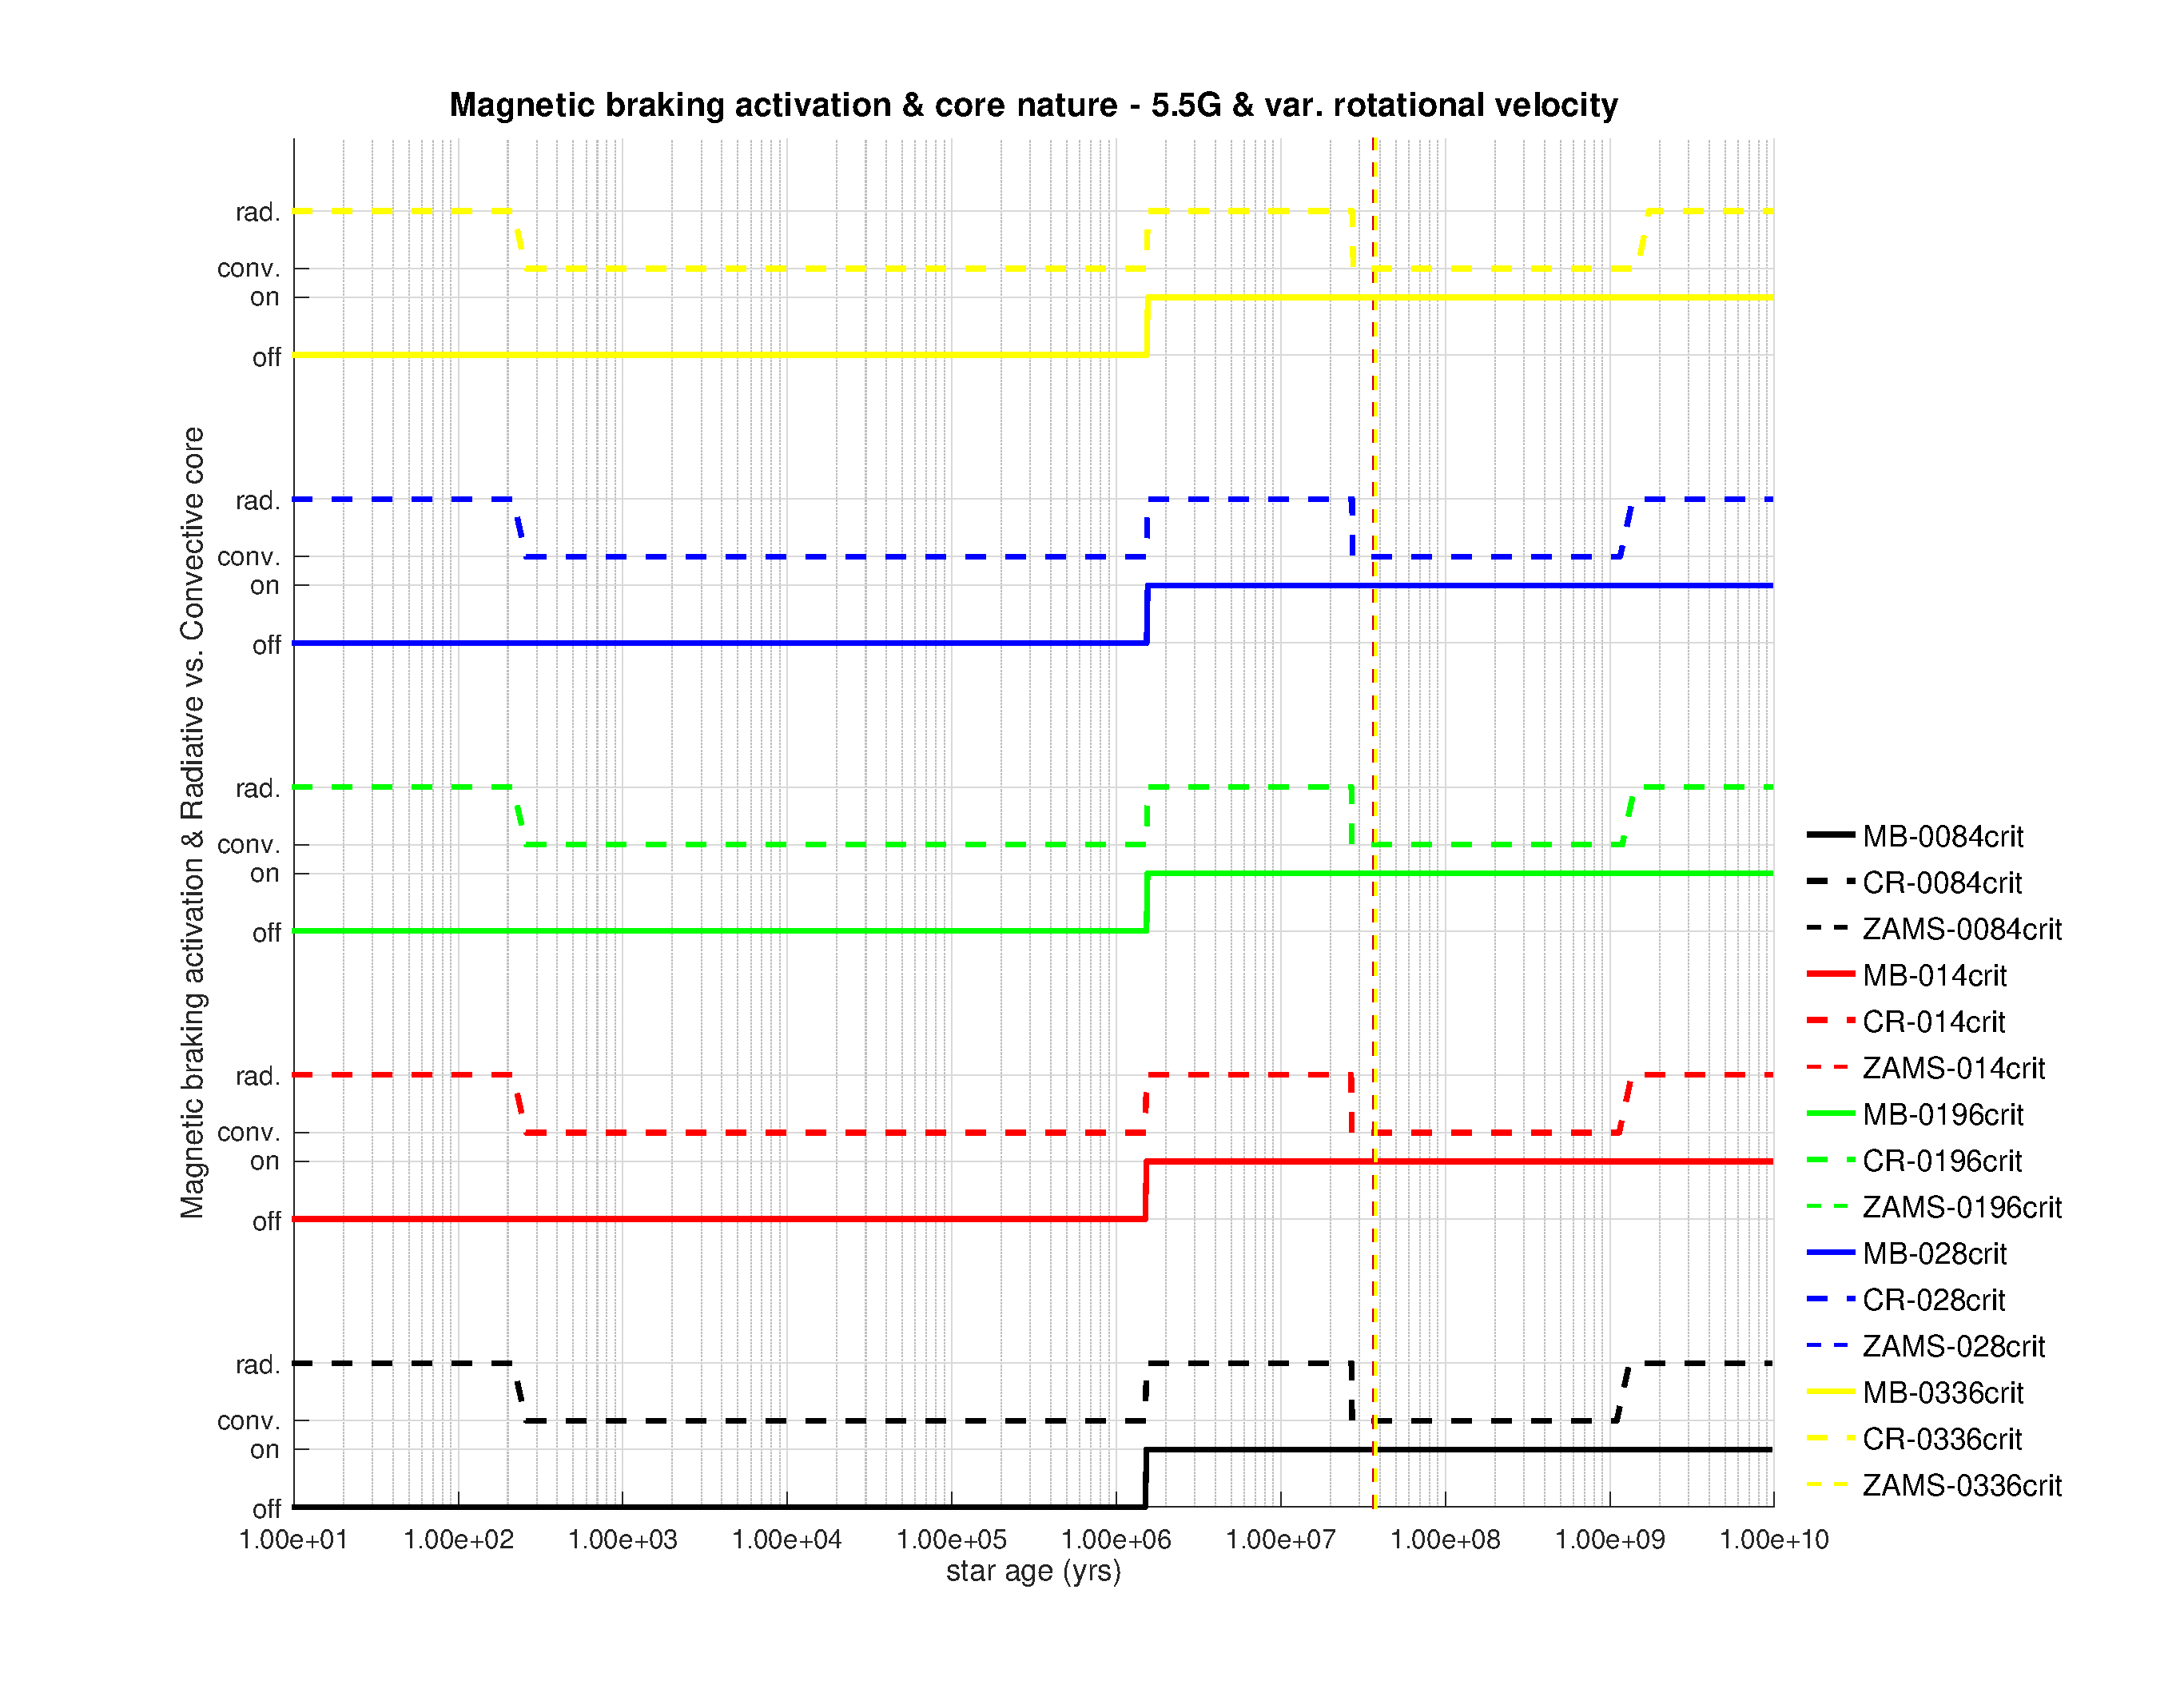
\includegraphics[trim = 30mm 15mm 20mm 15mm, clip,width=\textwidth]{figures/mb_act_var_vel_5_5g.eps}
    \label{fig:subim35}
    \end{subfigure}
    \begin{subfigure}[h]{0.47\textwidth}
    \includegraphics[width=\textwidth]{figures/blank.eps}
    \label{fig:subim36}
    \end{subfigure}
\caption{Grid showing the evolution of magnetic braking activation, as a function of time and the existence of a radiative core for several 1 $M_{\sun}$ models. Each figure shows a set of models in which the magnetic field with intensity has been fixed and $\Omega / \Omega_{crit}$ varies between 0.0084 and 0.0336. The dashed lines make reference to the ZAMS.}
\label{fig:grid_mb_act}
\end{figure*}




\section*{Acknowledgements}
We are pleased to acknowledge Jieun Choi her kindness in responding to the different questions about her work which were aimed to reproduce the results obtained as far as Li is concerned, and also for allowing us access to the MESA files she used. Also we very much appreciate the expert support provided by Elisa Delgado-Mena during the process review of this document. Similarly, we wish also to thank Matteo Cantiello and Bill Paxton for their very valuable support in the development of the magnetic braking routine in MESA. Finally, we wish to acknowledge the generous work and help offered by the MESA community.

%%%%%%%%%%%%%%%%%%%%%%%%%%%%%%%%%%%%%%%%%%%%%%%%%%

%%%%%%%%%%%%%%%%%%%% REFERENCES %%%%%%%%%%%%%%%%%%

% The best way to enter references is to use BibTeX:

\bibliographystyle{mnras}
%\bibliography{magbrlitium} % if your bibtex file is called example.bib
\bibliography{mblithium}


% Alternatively you could enter them by hand, like this:
% This method is tedious and prone to error if you have lots of references
%\begin{thebibliography}{99}
%\bibitem[\protect\citeauthoryear{Author}{2012}]{Author2012}
%Author A.~N., 2013, Journal of Improbable Astronomy, 1, 1
%\bibitem[\protect\citeauthoryear{Others}{2013}]{Others2013}
%Others S., 2012, Journal of Interesting Stuff, 17, 198
%\end{thebibliography}

%%%%%%%%%%%%%%%%%%%%%%%%%%%%%%%%%%%%%%%%%%%%%%%%%%



% Don't change these lines
\bsp	% typesetting comment
\label{lastpage}
\end{document}

% End of mnras_template.tex